\chapter{Simulation-based inference for strong gravitational lensing} \label{cha:lensing}

\todo{
	\begin{itemize}
		\item Resolution of Fig.  3.13, 3.14, 3.16, 3.17, 3.18, 3.19
		\item Merge methodology + write tasks subdivision
		\item Polish pop results
	\end{itemize}
}

Precision analysis of galaxy-galaxy strong gravitational lensing images provides a unique way of characterizing small-scale dark matter halos, and could allow us to uncover the fundamental properties of dark matter's constituents. Recently, gravitational imaging techniques made it possible to detect a few heavy subhalos. However, gravitational lenses contain numerous subhalos and line-of-sight halos, whose subtle imprint is extremely difficult to detect individually. Existing analyses are reliant on likelihood-based methods like Markov-chain Monte Carlo or nested sampling, and generally require various compromises to the realism of lensing models for the sake of computational tractability, such as ignoring the numerous other subhalos and line-of-sight halos in the system, assuming a particular form for the source model, compressing observations into hand-crafted summary statistics (\eg~a power spectrum of residuals), and requiring the noise to have a known likelihood function. 

Here we show that a simulation-based inference method called \gls*{tmnre} makes it possible to relax these requirements by training neural networks to directly compute marginal posteriors for parameters of interest from lensing images. By performing a set of proof-of-concept inference tasks on simulated data, first, we verify the accuracy of \gls*{tmnre} and show it can compute posteriors for subhalo parameters marginalized over populations of hundreds of substructures that would be undetectable on their own, as well as lens and source uncertainties. Second, we show how to perform hierarchical inference of the dark matter halo mass function cutoff mass from multiple lensing images. Furthermore, we show that since \gls*{tmnre} learns a posterior function it enables direct statistical checks that would be extremely expensive with likelihood-based methods. Our results show that the full subhalo and line-of-sight halo population must be included when measuring the properties of individual dark matter substructures with this technique, and that \gls*{tmnre} is able to put tight constraints on the mass of warm dark matter in the multi-keV regime. \gls*{tmnre} is well-suited for analyzing complex lensing data. These first analysis demonstrate that our framework is in principle able to extract the wealth of information regarding dark matter’s nature contained in existing lensing data and in the large sample of lenses that will be delivered by near-future telescopes.

\textit{This chapter is based on work from \cite{Montel:2022fhv, Coogan:2022cky}.}



\section{Introduction} \label{sec:sl-intro}

\paragraph*{Dark matter puzzle.} Over the past several decades, numerous astrophysical probes including rotational curves of spiral galaxies \citep{Rubin:1980zd}, galaxy-cluster dynamics \citep{Zwicky:1933gu}, cosmic microwave background \citep{Planck:2015fie}, gravitational lensing observations \citep{Taylor:1998uk}, have established \gls*{dm} as one of the major components of the universe, comprising about $85\%$ of the its mass. However, up to the present time, the fundamental nature of \gls*{dm} is still one of the key unresolved puzzle in physics. For many years, the \gls*{cdm} paradigm \citep{Peebles:1982ff} has been able to accurately reproduce vastly disparate large-scale observations across all epochs. In this model, \gls*{dm} is massive, neutral, non-relativistic, and collisionless. %The main prediction of the \gls*{cdm} paradigm is that structure formation is due to a hierarchical clustering process, guided by gravitational instability of \gls*{dm} density perturbations, originated from quantum fluctuations during inflation. 

Despite providing a stunning description of the observed distribution of matter on large scales ($>\order{\si{\Mpc}}$), the agreement between \gls*{cdm} predictions and observations at galactic and sub-galactic scales has been less clear. At present, there is continued debate over whether the known abundance of dwarf galaxies and the density profiles of low-mass galaxies are in tension with the predictions of $\Lambda$CDM (respectively dubbed the missing satellites problem \citep{Moore:1999nt,Klypin:1999uc} and the cusp-core problem \citep{deBlok:1997zlw}, reviewed in \citealp{Bullock:2017xww}).
Solutions to these tensions include the impact of baryonic processes, such as supernovae feedback and reionization processes \citep{Bullock:2010uy}, or alternative \gls*{dm} physics. %Baryonic processes from supernovae feedback and reionization processes suppress star formation in low-mass galaxies \citep{Bullock:2010uy}, resulting in most \gls*{dm} subhalos not containing sufficiently bright galaxies and thus being more difficult to detect. Furthermore, baryonic feedback can "flatten out" the core of a dark matter profile, since feedback-driven gas outflows produce a time-varying gravitational potential that transfers energy to the orbits of the collisionless dark matter particles

The latter approach requires an alteration of \gls*{dm} particle physics, such that large-scale predictions remain unaffected, but the number of small-scale substructures is suppressed. \Gls*{dm} models which are warm instead of cold \citep{Colin:2000dn,Hogan:2000bv, Lovell:2013ola}, collisional instead of collisionless \citep{Spergel:1999mh}, or quantum on macroscopic scales rather than classical \citep{Hu:2000ke} predict a diverse array of possible configurations of low-mass halos and could potentially resolve these tensions \citep{Buckley:2017ijx}. Unfortunately, light \gls*{dm} halos are difficult to probe as they are not expected to accumulate enough baryonic matter to form stars and hence are truly \emph{dark} \citep{Efstathiou:1992zz,Fitts:2016usl}. If \gls*{dm} has significant self-interactions, such halos might be detectable by searching for the self-annihilation or decay products of \gls*{dm} \citep{Adhikari:2022sbh}. However, even if such interactions are not present, light halos can potentially be probed through their irreducible gravitational effects. In this chapter we study one such probe: galaxy-galaxy strong gravitational lensing.

\paragraph*{Strong gravitational lensing as a dark matter probe.} In strong gravitational lensing, the gravitational field of a mass distribution acts as a \emph{lens} by magnifying and distorting the light flux coming from a background \emph{source} \citep{Kochanek:aa}. This leads to multiple magnified and distorted images of the source, as explained by general relativity. The effect is sensitive only to how matter is distributed, regardless of its physical nature (baryonic/DM), and thus provides a direct way of probing the distribution of \gls*{dm} at small scales (see \cite{Vegetti:2023mgp} for a recent review). 

Indeed, a \emph{perturber} (\ie, a subhalo or \gls*{los} halo lying somewhere between the observer and source) positioned near one of these images contributes additional, much more localized distortions, on top of the main lens mass distribution. By carefully analyzing the relationship between the multiple images of the source, the distortions from a perturber can be disentangled from possible variations in the source light and its properties can be measured. Moreover, a population of dark perturbers can collectively cause perturbations to images that can be detected statistically in order to constrain population-level parameters, such as the suppression scale in the the low-mass end of the \gls*{hmf}, which are dictated by the fundamental properties of \gls*{dm}. Therefore, gravitational lensing provides a pristine probe of small-scale structures and can in principle distinguish between \gls*{dm} scenarios.

\paragraph*{Strong lensing image analysis.}Various different methods have been suggested to analyse the effects of small-scale structures on lensing images \citep{Drlica-Wagner:2019aa}. These methods usually target two different types of lensing systems that differ in the lensed source: quadruply-lensed quasars, and extended background galaxies that get lensed into extended arcs or complete Einstein rings.

In the former case, the source is a nearly point-like quasar that is lensed into four compact images  (\emph{``quads''}). These images' positions and flux ratios comprise the summary statistics for these systems. The presence of a perturber near one of these images would cause anomalies in the ratios of their fluxes relative to what would be predicted assuming a smooth lens mass distribution. Evidence for flux ratio anomalies due to perturber was first found in \cite{Mao:1997ek}. Later, \cite{Dalal:2001fq} derived a statistical constraint on the substructure fraction in the lensing galaxies using a small sample of seven lensed quasars. \cite{Nierenberg:2014cga} showed that flux-ratio anomalies can also be used to detect individual low-mass subhalos. Several studies derived upper limits on the subhalo mass function %half-mode mass $\mhm$
\citep{Nierenberg:2017vlg}, also including perturbations due to \gls*{los} halos \citep{Gilman:2017voy, Gilman:2019nap}. Further investigations \citep{Hsueh:2016aih, Hsueh:2017zfs, Hsueh:2019ynk} pointed out the importance of correctly modeling baryonic structure in the main lens, in order to avoid systematic errors while constraining \gls*{dm} substructure abundance with flux-ratio anomalies. 

Here we focus on \emph{gravitational imaging}, which refers to the analysis of lenses with extended arcs \citep{Koopmans:2005ig,Vegetti:2008eg,Vegetti:2009gw}. The observation in this case consists of a whole image. On one hand, such images cover a larger area of the sky than the four point-like images in quads, potentially providing more sensitivity to detect perturbations due to perturbers, in the form of percent-level variations in the shape of the predicted lensed light based on a smooth lens model. On the other hand, extracting this information requires modeling the source galaxy's light, which generally has a complex morphology. The gravitational imaging technique was first introduced in \cite{Koopmans:2005nr} and further developed in \cite{Vegetti:2008eg, Vegetti:2009gw}. Its application to real data  has so far yielded to several detections of individual heavy ($>10^8 \si{\solmass}$) perturbers using deep, high-resolution observations in the optical from the \gls*{hst} and Keck as well as in radio data from Atacama Large Millimeter/submillimeter Array \citep{Vegetti:2010wa, Vegetti:2009cz, Vegetti:2012mc, Hezaveh:2016ltk,Diego:2022mii}. Moreover, measurements and non-detections of individual perturbers in samples of gravitational lens systems can be converted to constraints on the (sub)halo mass function and thus dark matter's properties \cite{Vegetti:2014lqa, Vegetti:2018dly,Ritondale:2018cvp}.

Established gravitational imaging analyses such as the method in \cite{Vegetti:2008eg,Hezaveh:2016ltk} use \emph{likelihood-based} inference to infer the properties of perturbers. The central mathematical object in such approaches is the likelihood, a probabilistic model $p(\data \mid \param)$ for the data $\data$ given some parameters $\param$ for the lens, source, perturbers and possibly other (hyper)parameters.\footnote{For example, the hyperparameters could include the pixel size for pixelated sources or strength of source regularization.}   
Likelihood-based tools, such as \gls*{mcmc} or nested sampling~\citep{Skilling:2004pqw}, do not directly produce marginal posteriors but instead compute the \emph{joint posterior} $p(\param \mid \data_0)$, which must then be marginalized over. 

The computational expense of sampling from the high-dimensional joint posterior imposes restrictions on the realism of lensing models that can be analyzed. One such restriction common to most analyses is to  assume a particular form of the noise and source model so that the source uncertainties can be excluded from the sampling and marginalized over analytically \citep{Hezaveh:2016ltk,Vegetti:2008eg,Vegetti:2009cz,Vegetti:2010wa,Vegetti:2012mc}. This makes it difficult to explore more complex source models described by \eg~generative machine learning methods or noise artifacts like cosmic ray streaks that cannot be described by an analytic likelihood.

An additional difficulty with likelihood-based analyses is that each run of \gls*{mcmc} or nested sampling produces posterior samples for just a single observation. Directly exploring the systematics, biases and other statistical properties of a particular lensing model is thus extremely time-consuming, necessitating rerunning posterior sampling many times for different input observations. This also makes analyses such as mapping perturber measurement sensitivity costly. It is noteworthy that recently \cite{Nightingale:2022bhh} pushed to the limits how far one can feasibly go using likelihood-based analyses, fitting 54 images with 5 different mass models.

Likelihood-based analyses also typically assume no more than two perturbers are present in each image. Allowing for $n$ perturbers would cause the joint posterior to become highly multimodal, with approximately $n!$ modes due exact invariance of the observation under relabeling of perturbers. In these frameworks, it is then challenging to perform statistical inference of quantities such as the posterior of mass and position of a single heavy subhalo in the presence of a population of lighter perturbers, or the posterior for substructure population-level parameter of interest, marginalizing over all source, lens, and substructures parameters to get the marginal of interest.

\emph{Transdimensional Bayesian inference} \citep{Brewer:2015yya,Daylan:2017kfh} partially overcomes this traditional likelihood-based methods' challenge, by using transdimensional \gls*{mcmc} to infer the probabilities of different possible populations of perturbers, albeit at substantial computational cost. 

An alternative strategy involves linearising the gravitational potential via a \emph{Taylor expansion} of the lens equation. By employing a Taylor expansion, it becomes feasible to capture all small-scales \gls*{dm} substructures without the need to parameterise them directly in the likelihood function \citep{Vegetti:2008eg, Koopmans:2005nr, Galan:2022ifd}. This technique is therefore able to account for the full \gls*{dm} subhalo population (a part from the effects due to the curl-component induced by multi-plane lensing effects).

Another approach is to circumvent measuring individual perturbers by instead engineering \emph{summary statistics} from first principles, such as the convergence \gls*{ps} for different subhalo populations  \cite{DiazRivero:2017xkd, DiazRivero:2018aa, Brennan:2018jhq}, and also for \gls*{los} populations \cite{CaganSengul:2020nat}. However, this approach is not directly applicable to observations, because we do not have access to the true displacement field from the data. Building upon this, it is possible to relate the \gls*{ps} of the surface brightness fluctuations in strong lens images to the lens potential fluctuations arising from \gls*{dm} distribution that contribute to the convergence \gls*{ps} \cite{Chatterjee:2017orx, Cyr-Racine:2019aa, Bayer:2018vhy}. Another summary statistic that has been employed is the residuals between the image and best-fit reconstruction excluding substructure, that is related to the (sub)halo mass function parameters. In particular, this summary statistic has been successfully employed to constrain the \gls*{hmf} suppression scale using \gls*{abc}  \cite{Birrer:2017rpp, He:2020rkj}. This approach reduces the dimensionality of the problem and enable inference of the collective effects of a large number of low-mass substructures at the statistical level. However, it is unknown how much information such approach discards. 

%In fact, inferring marginal posteriors for the \gls*{hmf} cutoff requires marginalizing over all source, lens, and substructures parameters to get the marginal likelihood for the population-level parameter of interest, thus involving a time-consuming exploration of a very high-dimensional parameter space for complex realistic models. T
%Statistical inference of perturber parameters $\vec{\theta}_\mathrm{sub}$ such as mass and position given an observation $\data_0$ amounts to computing marginal posteriors $p(\vec{\theta}_\mathrm{sub} \mid \data_0)$ by means of \gls*{mcmc} or nested sampling~\citep{Skilling:2004pqw}. 
%\newline , a likelihood-free inference method based on a rejection algorithm \citep{Grazian:2019aa}

Another class of methods that has developed in recent years uses \emph{neural networks} to measure lens parameters \citep{Hezaveh:2017sht, PerreaultLevasseur:2017ltk,  Morningstar:2019szx}, quantifying the structure of gravitational lens potential \citep{Vernardos:2020aa}, detect individual subhalos \citep{Rivero:2020aa}, distinguish different types of \gls*{dm} substructure based on their lensing signatures \citep{Alexander:2019puy}, and classify whether each pixel in an image contained a subhalo in a given mass bin \cite{Ostdiek:2020cqz,Ostdiek:2020mvo}. Still, these methods need lots of data to amortize over all possible variations in lensing systems. In fact, amortized methods learn the posterior for any data, generated by any parameter over the whole range of the prior. But learning an amortized posterior is unnecessary if only a small range of parameters are consistent with a target observation.


\paragraph*{This work.} In this work, we demonstrate that a \gls*{sbi} \citep{Cranmer:2019eaq} method called truncated marginal neural ratio estimation \citep{Miller:2020hua,Miller:2021aa}, from here on \gls*{tmnre}, can circumvent these inference challenges to \emph{measure the properties of individual perturbers} and to \emph{measure the suppression scale of the subhalo \gls*{hmf} directly from images by combining multiple observations}.

In a nutshell, \gls*{sbi}, first presented in Chapter~\ref{cha:sbi}, refers to a class of statistical inference methods that use the output of a stochastic simulator that need not have a known likelihood. In particular, \gls*{nre}, first presented in \cite{Hermans:2019ioj}, trains a neural network to map from observations directly to \emph{marginal posteriors} for a specified subset of model parameters (\eg~the position and mass of a perturber). This bypasses the requirement of likelihood-based inference to sample the joint posterior. In contrast to methods like \gls*{abc}, this also removes the need to engineer summary statistics \citep{He:2020rkj} as they are in effect learned directly from the training data. Since \gls*{nre} learns a marginal posterior \emph{function}, it is straightforward to check the statistical properties of the inference results for different observations. \gls*{tmnre} further extends \gls*{nre} by focusing training data generation in the regions of parameter space most relevant for analyzing a particular observation over a sequence of inference rounds. This substantially reduces the number of simulations required to train the inference network as well as the required network complexity.

Several other works have applied \gls*{sbi} to substructure lensing. In \cite{Zhang:2022djp} a likelihood-ratio estimation technique similar to \gls*{tmnre} was employed to measure density profile parameters of subhalos from images. \cite{Wagner-Carena:2022mrn} recently applied neural posterior estimation to measure the subhalo \gls*{hmf} normalization in mock lensing images using real galaxy images as sources. \cite{Brehmer:2019jyt} utilized a ``likelihood-based'' \gls*{sbi} method requiring the simulator's score\footnote{
    The score is the derivative of the log-likelihood for a given observation with respect to the model's parameters.
} to measure the slope and normalization of a subhalo \gls*{hmf} in simple mock images.
%For the statistical analysis we employ \gls*{tmnre}. Developed by \citet{Hermans:2019ioj} and \citet{Miller:2020hua}, \gls*{mnre} is a neural \gls*{sbi} method that makes it possible to learn the marginal posterior approximation for a specified subset of model parameters of interest directly from the full input data that, in our case, corresponds to the observed lensed images, without the need for hand-crafted summary statistics. This method improves the simulator efficiency and the quality of inference. Moreover, \gls*{mnre} is amortized, which  enables important statistical consistency tests, which would have been extremely expensive with likelihood-based inference, like the expected coverage test we employ in Section~\ref{subsec:test}. Up to now, this approach has been applied in simplified modeling frameworks: \citet{Hermans:2019ioj} focuses on recovering the Einstein radius of a gravitational lens marginalizing over 15 source and lens mass distribution parameters, whereas \citet{Brehmer:2019jyt} estimates the slope and normalization of a \gls*{cdm} subhalo mass function. \gls*{sbi} using neural posterior density estimator and hierarchical inference have also been employed in \citet{Wagner-Carena:2022mrn} to infer the \gls*{cdm} subhalo mass function normalization from a set of strong-lensing images, generated using real galaxy images as a source model, including realistic observational noise effects from \gls*{hst} and accounting for the mean expected convergence from \gls*{los} halos. 
%\Gls*{tmnre} is able to \emph{target} the inference to a specific observation at hand rather than amortize over all possible parameters combinations, by successively focusing simulations on the parameter regions that are most relevant for the inference problem \citep{Miller:2021aa}.
%This targeted approach is more efficient when most posterior density is concentrated compared to the prior density, which is the case for lens and source parameters.
%This truncation method applied to strong-lensing images was proposed in \citet{Karchev:2021fro} and used in \citet{Coogan:2020yux, Coogan:2022cky} to learn marginal posterior approximations for individual subhalo parameters, marginalizing over lens and source uncertainties given an observation. It has also been recently applied to analysis of the CMB \citep{Cole:2021gwr}.

The present work complements these efforts in several ways. As far as measuring individual perturbers complements is concerned, first, it offers a path towards cross-checking current substructure measurements under different modeling assumptions. Second, inference based on perturbers provides a level of interpretability beyond measuring subhalo \gls*{hmf} parameters directly from images, and moreover the opportunity to test different \gls*{dm} models through measuring the properties of individual subhalos. Third, measuring the heaviest subhalos in an observation enables modeling them explicitly in lensing simulations, which could reduce the training data requirements and improve inference accuracy for direct subhalo \gls*{hmf} measurements.

 On the other hand, as far as measuring the suppression scale of the subhalo \gls*{hmf} directly from an ensemble images is concerned, first, this work demonstrates the sensitivity of the \gls*{tmnre} approach to the \gls*{hmf} suppression scale. Second, it illustrates the importance of combining the information coming from different observations in the statistical analysis, especially in light of near-future data delivery. Currently, there are around a hundred strong lensing observations suitable for substructure inference, most of which come from the SLACS \citep{Bolton:2005nf} and BELLS \citep{BOSS:2011bef} surveys. In the near future, new and future telescopes like JWST \citep{Gardner:2006ky}, ELT \citep{Simon:2019aa}, Euclid \citep{Refregier:2010ss, EUCLID:2011zbd}, SKA \citep{Koopmans:2004gf}, and LSST \citep{LSSTDarkEnergyScience:2020oya} will greatly increase the quality of data suitable for gravitational imaging analyses as well as its quantity, from $\order{100}$ to $\order{10^5}$ images \citep{Collett:2015roa, McKean:2015aa}.

This chapter is organized as follows. In Section~\ref{sec:sl-model} we describe our strong lensing model, which uses an analytic source and main lens in conjunction with well-motivated perturber models. We then carry out two distinct analysis tasks with \gls*{tmnre}: inference of the parameters of a single subhalo in a lensing image Section~\ref{sec:results-sub}, and hierarchical inference of the halo mass function cutoff scale from an ensemble of lenses Section~\ref{sec:results-pop}. This work will help form the basis for \gls*{sbi}-based analysis of strong lensing images as a dark matter probe in existing and future lensing data.

% Our analysis begins in Section~\ref{sec:results-sub}, where we show that \gls*{tmnre} is capable of recovering posteriors for a subhalo's mass and position in the limit where they are analytically-calculable. We then gradually complexify our inference tasks, first accounting for the fact that the source and lens parameters are unknown and later by incorporating a population of light perturbers to marginalize over.  This work paves the way for combining the presented statistical analysis with more realistic strong lensing source models and for future applications to real high-resolution data in upcoming works.



\section{Modelling strong lensing observations}  \label{sec:sl-model}

Here we review how we model strong lensing images. We implement our lensing model in \texttt{PyTorch} \citep{pytorch} so that we can leverage GPUs to rapidly generate large numbers of observational data (a single-channel telescope image).

\subsection{The physics of strong lensing}
Before delving into modelling details, we briefly summarise the key points of the physics of gravitational lensing, referring the reader to \eg~\cite{Meneghetti:2016aa} for a more detailed overview. In strong-lensing systems the mass distribution of a foreground galaxy gravitationally lenses the light rays coming from a background source, resulting in an arc-like image in the case of an extended galaxy source. We assume that mass densities are low enough to treat the gravitational field of the matter in the image plane in the Newtonian approximation of \gls*{gr}. In this case the metric is fully characterized by the lens' gravitational potential $\psi$. We also adopt the thin lens approximation, which assumes all the lens mass lies in a single \emph{image plane} and all the source light is emitted from a \emph{source plane}. 

We will be using $\vec{\xi}\equiv(\xi_x, \xi_y)$ and $\vec{x}\equiv(x, y)$ as two-dimensional angular coordinates in the image and source planes respectively, and use $z$ to indicate distances along the orthogonal dimension. Since the image plane covers a small angular patch of the sky and the lensing deflections are small in the Newtonian limit, the coordinate system can be treated as Cartesian.

The configuration, then, is determined by two fields: the distribution of surface brightness in the source plane, $\beta(\vec{x})$, and the distribution of mass in the image plane, described by the projected potential:
\begin{equation}
	\Psi(\vec{\xi})\equiv \int_{-\infty}^{\infty} \psi(\xi_x, \xi_y, z) \mathrm{d}z
\end{equation}

Under these assumptions, the source-plane coordinate to which a light ray through the image plane traces back is given by the simple \emph{lens equation}
\begin{equation} \label{eq:gl-lensing}
    \vec{x} = \vec{\xi} - \vec{\alpha}(\vec{\xi}) \, .
\end{equation}
The displacement field $\vec\alpha$ is determined by the projected potential:
\begin{equation} \label{eq:disp_grad}
    \vec{\alpha}(\vec{\xi}) = \frac{D_{LS}}{D_S} \frac{2}{c^2} \frac{\vec{\nabla}_{\vec{\xi}} \Psi(\vec\xi)}{D_L} \, ,
\end{equation}
where the gradient is taken in the image plane and should have dimensions of inverse length, whence the introduction of the observer-lens angular diameter distance $D_L$. The expression also involves the angular diameter distances $D_{LS}$ (from the lens to the source), and $D_S$ (from the observer to the source).\footnote{
    We compute angular diameter distances with \texttt{astropy}~\citep{Astropy:2013muo,Astropy:2018wqo} using the flat cosmology from Planck \citep{Planck:2018vyg}.
} 
We illustrate in Figure~\ref{fig:gl-lensing} the geometry of the system.

\begin{figure*}
    \centering
    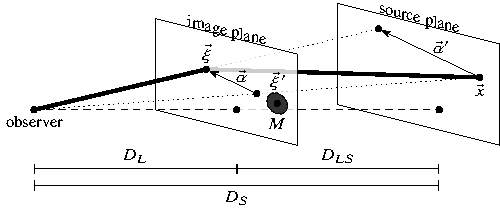
\includegraphics[width=0.8\linewidth]{Figures/GL-lensing.pdf}
    \caption{Thin lens geometry. The lensing mass $M$ located at $\vec\xi'$ bends the light ray (thick line) emanating from the point $\vec x$, so that to the observer it looks like it is coming from the direction of $\vec\xi$ . General relativity predicts the deflection angle $\vec\alpha'$  \emph{as viewed from the image plane} based on the mass $M$ and the impact parameter $\vec b = \vec \xi - \vec \xi '$. It then has to be rescaled by $\frac{D_{LS}}{D_S}$ to obtain the displacement field $\vec\alpha$ (as viewed by the observer) for use in Equation~\eqref{eq:gl-lensing}. Angles are all assumed to be small enough that they can be used for Euclidean calculations. The dashed line is the optical axis perpendicular to the planes and connects the origins of the coordinate systems for each plane. The figure is a reproduction of Figure 2 in \cite{Karchev:2021fro}.}
    \label{fig:gl-lensing}
\end{figure*}

From a computational standpoint it is more convenient to represent Equation~\eqref{eq:disp_grad} as an integral. Using the Poisson equation $\nabla_2 \Psi= 4\pi G\rho$ and setting appropriate boundary conditions:
\begin{equation} \label{eq:disp_int}
    \vec{\alpha}(\vec{\xi}) = \frac{4 G}{c^2} \frac{D_{LS}}{D_L \, D_S} \int \Sigma(\vec{\xi}') \frac{\vec{\xi} - \vec{\xi}'}{\mid\vec{\xi} - \vec{\xi}'\mid^2}   \mathrm{d}{(D_L \vec{\xi}')} \, ,
\end{equation}
where the integral is performed over the image plane, and where $c$ is the speed of light and $G$ is the gravitational constant.

Here $\Sigma$ is the projected (surface) mass density related to the 3D mass density $\rho$ by an integration along the coordinate perpendicular to the lens plane $z$:
\begin{equation}
	\Sigma(\vec\xi) \equiv \int_{-\infty}^{\infty} \rho({\xi}_x, {\xi}_y, z) \mathrm{d}{z},
\end{equation}
similarly to the expression for the projected potential.

The expression in Equation~\eqref{eq:disp_int} can be simplified by introducing the convergence $\kappa$ in terms of the critical surface density $\Sigma_{\mathrm{cr}}$:
\begin{equation}
    \kappa(\vec{\xi})=\cfrac{\Sigma(\vec{\xi})}{\Sigma_{\mathrm{cr}}},
    \quad \Sigma_{\mathrm{cr}}\equiv\cfrac{c^2}{4\pi G}\cfrac{D_S}{D_L D_{LS}} \, .
\end{equation}
If  $\kappa > 1$, a lens can form multiple images \cite[Section 2.6]{Meneghetti:2016aa}. The threshold for this to happen is set by the critical surface density, and it is evident from its expression that for a fixed distance to the lens ($D_L $) further away sources  ($D_S$) are lensed more easily, since they require smaller deflections.

Furthermore, it can be shown that the convergence $\kappa$ is related to the isotropic part of the trace of the Jacobian of the lensing transformation through
\begin{equation}\label{eq:lens-jacobian}
	\frac{\dd{\vec{x}}}{\dd{\vec{\xi}}} = \mqty(\dmat[0]{1-\kappa, 1-\kappa}) - \mqty(\gamma_1 & \gamma_2 \\ \gamma_2 & -\gamma_1),
\end{equation}
where the second part is the shear (discussed more in details in Section~\ref{subsec:sl-model-lens}).
Another important quantity is the inverse of the Jacobian's determinant, the magnification
\begin{equation}
	\mathcal{M} \equiv \mid\frac{\dd{\vec{\xi}}}{\dd{\vec{x}}}\mid  = \qty[(1-\kappa)^2 - \qty(\gamma_1^2 + \gamma_2^2)]^{-1},
\end{equation}
which is a measure of how much the solid angle spanned by the source is enlarged, or equivalently, of how gravitational focusing directs a larger fraction of the energy radiated by the source to the observer \cite{Bartelmann:1999yn}. Thus, when the convergence $\kappa$ and the shear $\gamma$ are equal or greater than unity, sources are \emph{strongly} magnified, and we can use the magnitude of the magnification to differentiate between \emph{strong} from \emph{weak} lensing regimes.

While lensing does change the apparent solid angle of a source, it is worth noting that it conserves energy, since it merely alters the trajectories of photons rather than creating or destroying them. As a result, the surface brightness $\beta(\vec{\xi})$ in the image plane is equal to the surface brightness at the point to which it traces back in the source plane (assuming one isolated source):
\begin{equation}
    \beta(\vec{\xi}) = \beta(\vec{x}(\vec{\xi})) \, .
\end{equation}

%It is important to note, however, that lensing does not create or destroy photons (and thus, conserves energy.}). Thus, the amount of light arriving at the observer is proportional to the area \emph{in the image plane} that the source subtends, which effectively acts as a collecting area for light that is then simply rerouted just as with conventional lenses. This means that \emph{lensing conserves surface brightness} around infinitesimal points, and thus the surface brightness registered by the observer (in the absence of other sources) is
%\begin{eq}
%	\sbr(\ximg) = \sbr(\x\qty(\ximg)).
%\end{eq}
%
%It is obvious from this expression that the lens and the source are entirely degenerate: for any observation there is for every deflection field (that does not form multiple images!) a surface brightness configuration that can reproduce the observation. The reverse (that one can find deflection fields that map distinct sources to the same image) is also sometimes true, giving rise to the mass-sheet \citep{masssheetdegeneracy} and source-position degeneracies \citep{sourcepositiontransformation} (the latter being more general but approximate). As a consequence, the spatial scale of the source cannot be conclusively determined (in the absence of time-delay data \ered{or additional constrants on the lens mass profile}) since a sheet of constant mass density could be magnifying it uniformly by an arbitrary amount \citep{lensing-short}.


\bigskip

Given the physics of strong lensing, in order to fully specify a strong-lensing model we then need two main ingredients: the lens model, which describes the total mass distribution of the lens, and the source model, which describes the surface brightness profile of the background source. It is common to split the lens model into a macroscopic smooth component (main lens and external shear) and a substructure\footnote{Throughout this thesis, we use the terms `small-scale structures', `substructures', and `low-mass halos' when considering both subhalos of the main lens and line-of-sight halos.} component, due to subhalos and line-of-sight halos. Each lensing ingredient can be directly superimposed by summing their respective displacement fields in the lens plane:
\begin{equation}
    \vec{\alpha} = \vec{\alpha}_\mathrm{lens} + \vec{\alpha}_\mathrm{ext} + \sum_{i=1}^{N_{\mathrm{sub}}} \vec{\alpha}_\mathrm{sub,i} + \sum_{i=1}^{N_{\mathrm{los}}} \vec{\alpha}_\mathrm{los,i}.
\end{equation}
In the following sections, we will describe each component of the model we use to simulate mock images of gravitational lenses: the source, the main lens, the dark matter perturbers, and instrumental noise. 


\subsection{Source model} \label{subsec:source}
To model the surface brightness of the source galaxy, we adopt the widely-used Sérsic profile \citep{Sersic:1963aa}. The surface brightness distribution is parameterized by 
\begin{equation}\label{eq:sersic}
    \beta(\vec{x})=I_e \exp{-k_n\left[\left(\cfrac{R(\vec{x})}{r_e}\right)^{1/n}-1\right]},
\end{equation}
where $I_e$ is the surface intensity at the half-light radius $r_e$. The radial parameter $r(\vec{x})=\sqrt{r_x^2+r_y^2}$ is the length of the elliptical radial coordinate vector
\begin{equation}
    \begin{pmatrix} 
        r_x \\ r_y 
    \end{pmatrix} = 
    \begin{pmatrix} 
      \sqrt{q_s} & 0 \\ 0 & 1/\sqrt{q_s} 
    \end{pmatrix} 
    \begin{pmatrix} 
        \cos\phi_s & \sin\phi_s \\ -\sin\phi_s & \cos\phi_s 
    \end{pmatrix} 
    \begin{pmatrix} 
        x - x_{0,s} \\ y - y_{0,s} 
    \end{pmatrix},
\end{equation}
which depends on the source's position angle $\phi_s$, axis ratio $q_s$, and center of light position $(x_{0,s}, y_{0,s})$. 

The normalization $k_n$ is related to the index $n$ by an implicit transcendental equation in terms of the complete and lower incomplete gamma functions $2\gamma(2n, k_n)=\Gamma(2n)$. We use the expansion in series from \cite{Ciotti:1999zs}, 
\begin{equation}
    k_n \approx 2 n - \frac{1}{3} + \frac{4}{405 n} + \frac{46}{25515 n^2} + \frac{131}{1148175 n^3} - \frac{2194697}{30690717750 n^4} \, .
\end{equation}
valid over a wide range of indices, $n>0.36$. For typical galaxies $1/2 < n < 10$.

Therefore, our source model is parametrised by seven variables that we collect in the vector $\bm \theta_s\equiv\{I_e, r_e, x_{0,s}, y_{0,s}, q_s, \phi_s, n\}$. We fix the source's redshift to $z_\mathrm{source} = 2$.

\subsection{Main lens model}\label{subsec:sl-model-lens}

%\footnote{
%    Throughout our work,  we use the terms “simulated data” for data used during inference and “mock observations” for the simulated data that we analyse.
%    }     
    
We adopt the \gls*{sple} model for the main lens galaxy, which is capable of modeling the gravitational potentials of strong lenses to near the percent level~\citep{Suyu:2008zp}. Furthermore, the \gls*{sple} model has been shown to be a more adequate representation of the combined \gls*{dm} and baryon mass distribution in the inner regions of galaxies, to which strong lensing is most sensitive \citep{Suyu:2008zp}. The \gls*{sple} deflection field can be expressed in closed-form as a complex field $\alpha = \alpha_x + i \alpha_y$ \citep{Tessore:2015baa,ORiordan:2020aa}:
\begin{equation}
\begin{split}
    \vec{\alpha}^\mathrm{SPLE}(\vec{\xi}) = \theta_E & \frac{2 q_\mathrm{l}^{1/2}}{1 + q_\mathrm{l}} \left( \frac{\theta_E}{r} \right)^{\gamma - 2} e^{i \varphi} \\
    & \cdot \hypgeom\left( 1, \frac{\gamma - 1}{2}, \frac{5 - \gamma}{2}, -\frac{1-q_\mathrm{l}}{1+q_\mathrm{l}} e^{2 i \varphi} \right) \, .
\end{split}
\end{equation}
Here $(r, \varphi)$ are elliptical coordinates, related to the Cartesian coordinates $\vec{\xi}$ through a transformation parametrized by the lens' orientation $\phi_\mathrm{l}$, axis ratio $q_\mathrm{l}$ and position $(\xi_\mathrm{x, 0}, \xi_\mathrm{y, 0})$:
\begin{align}
    \begin{pmatrix} r_x \\ r_y \end{pmatrix} &= \begin{pmatrix} q_\mathrm{l}^{1/2} & 0 \\ 0 & q_\mathrm{l}^{-1/2} \end{pmatrix} \begin{pmatrix} \cos\phi_\mathrm{l} & \sin\phi_\mathrm{l} \\ -\sin\phi_\mathrm{l} & \cos\phi_\mathrm{l} \end{pmatrix} \begin{pmatrix} \xi_x - \xi_{x, 0} \\ \xi_y - \xi_{y, 0} \end{pmatrix} \, ,\\
    \tan \varphi &= \frac{r_y}{r_x}.
\end{align}

In the circular ($q=1$) isothermal ($\gamma=2$) case this reduces to $\alpha=\theta_E e^{i\varphi}$, \ie~is an isotropic constant, as is well-known. Since the hypergeometric function $\hypgeom$, however, is not implemented in \texttt{PyTorch}, we instead pretabulate its value as a function of $\phi_\mathrm{l}$, $q_\mathrm{l}$ and $\gamma$ and interpolate at runtime, as described in \cite{Chianese:2019ifk}. This results in very fast code with negligible output degradation.

The slope $\gamma$ has a complicated degeneracy with the size of the source \citep{Schneider:2013sxa,Schneider:2013wga}. Roughly, larger $\gamma$ values cause the spatial scale of the source to increase \citep[sec. 3.3]{Nightingale:2014aa}. For simplicity we fix $\gamma = 2.1$. In principle, inferring the slope is possible, but it requires more training data and leads to increased uncertainties in both lens and source parameters.

We also assume the lens galaxy's light has been perfectly subtracted, and fix its redshift to $z_\mathrm{lens} = 0.5$.

To account for the weak lensing due to large-scale structure located along the line of sight to the source, we also include an external shear component, which is constant across the image plane:
\begin{equation}
    \vec{\alpha}^\mathrm{shear}(\vec{\xi}) = \begin{pmatrix} \gamma_1 & \gamma_2 \\ \gamma_2 & -\gamma_1 \end{pmatrix} \vec{\xi} \, .
\end{equation}

Our main lens model thus has seven parameters: the \gls*{sple} parameters $(\xi_{x, 0}, \xi_{y, 0}, \phi_\mathrm{l}, q_\mathrm{l}, \theta_E)$ and the external shear parameters $(\gamma_1, \gamma_2)$, which we denote collectively with $\bm \theta_l$.

\subsection{Small-scale structures model} \label{subsec:substructure}

\begin{figure}
	\centering
	\begin{subfigure}[b]{0.5\linewidth}  
	\centering
	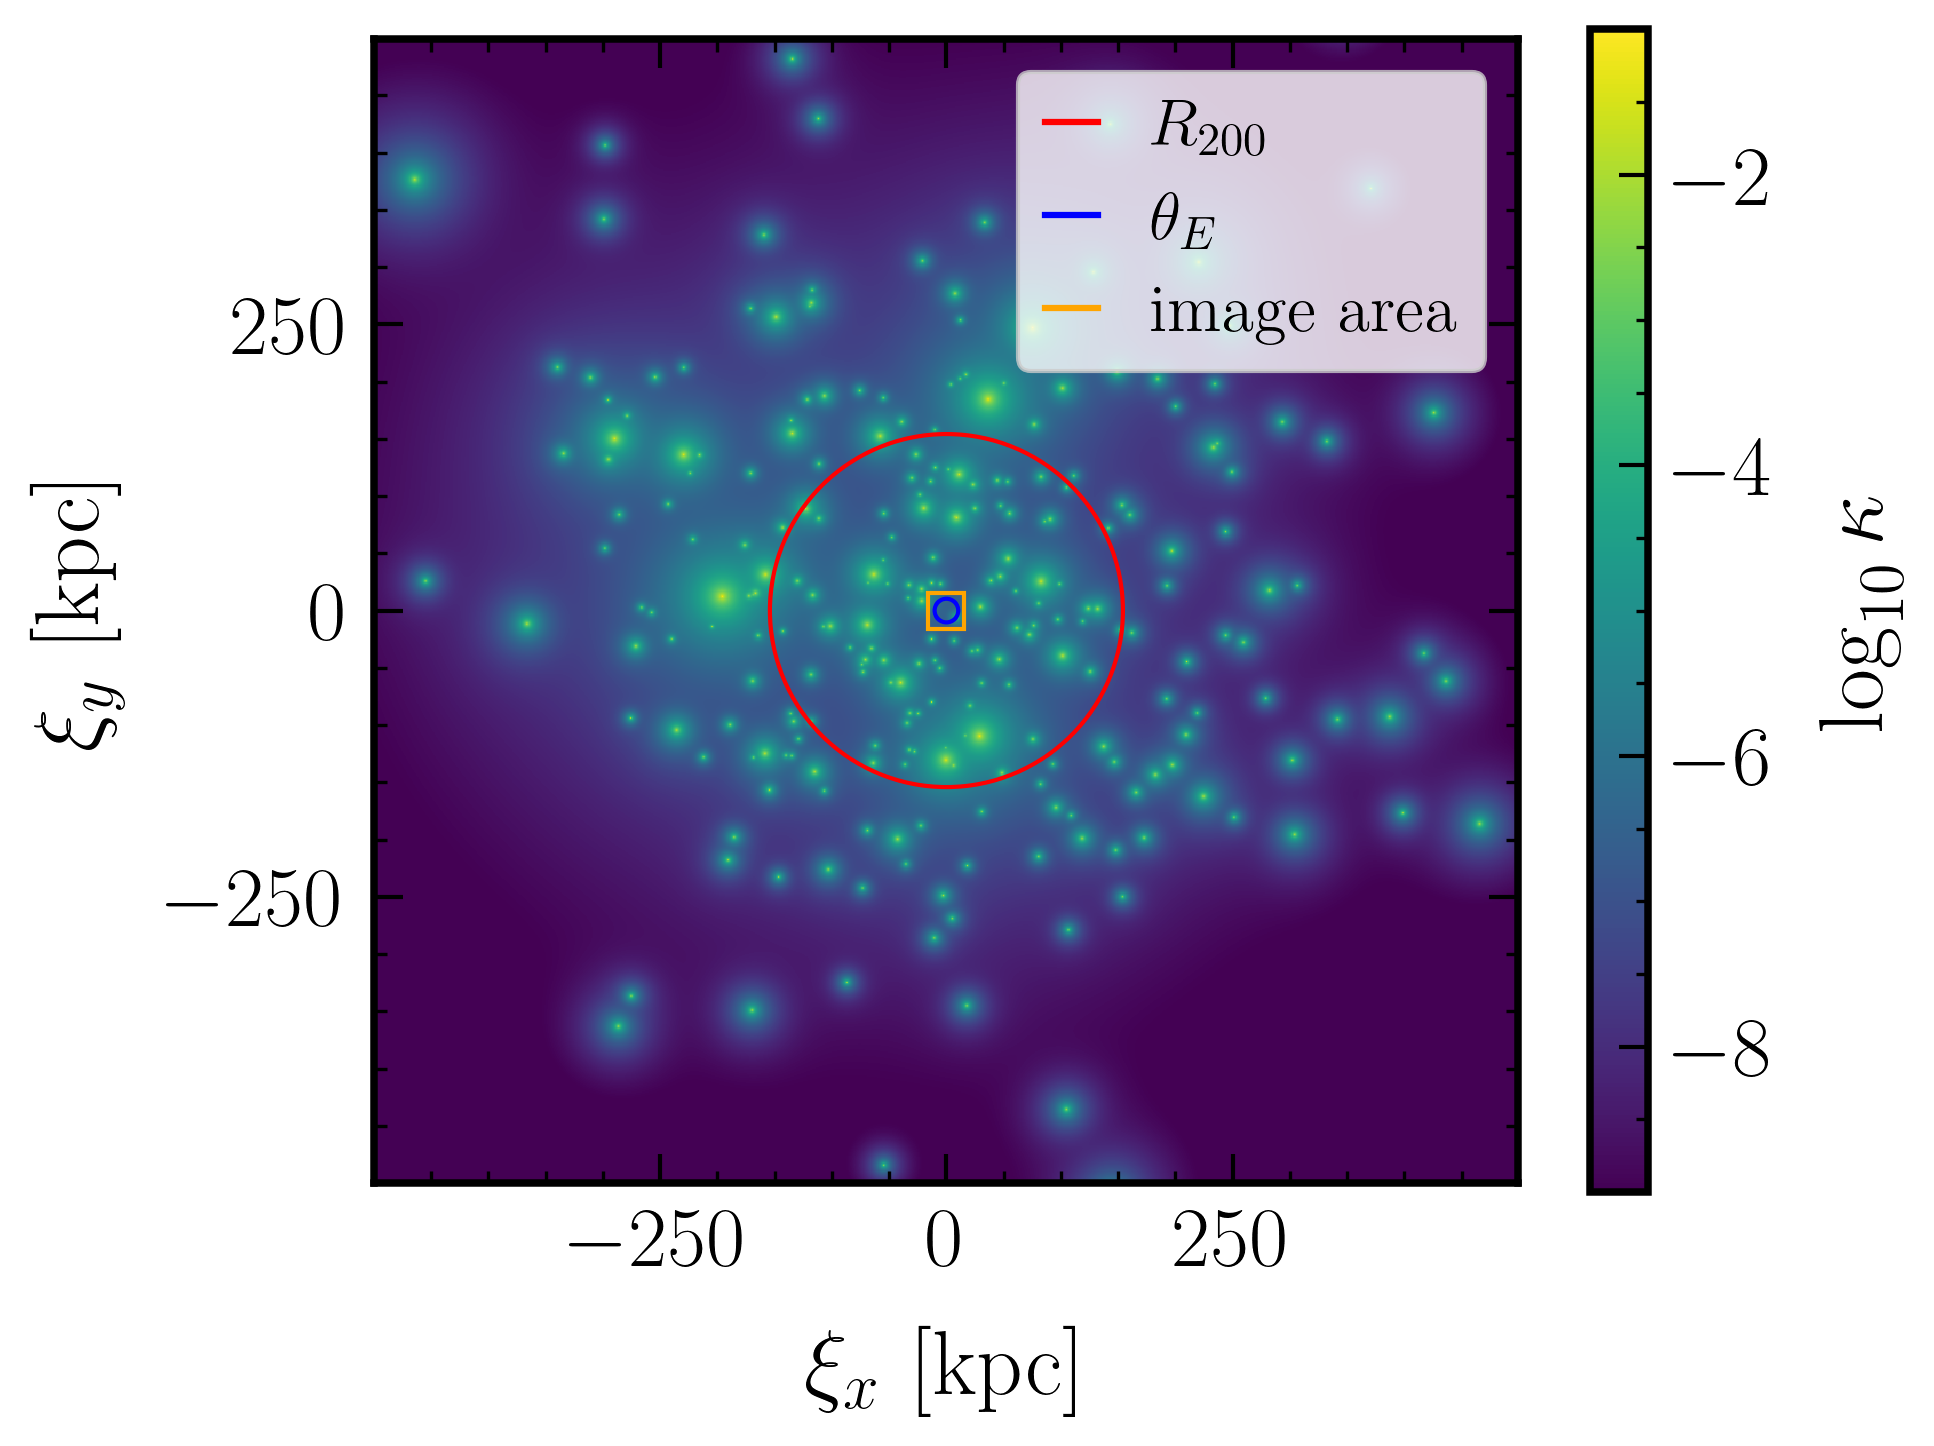
\includegraphics[width=\linewidth]{GL-sub-convergence.png}
	\end{subfigure}
	\hfill
	\begin{subfigure}[b]{0.46\linewidth}
	\centering
	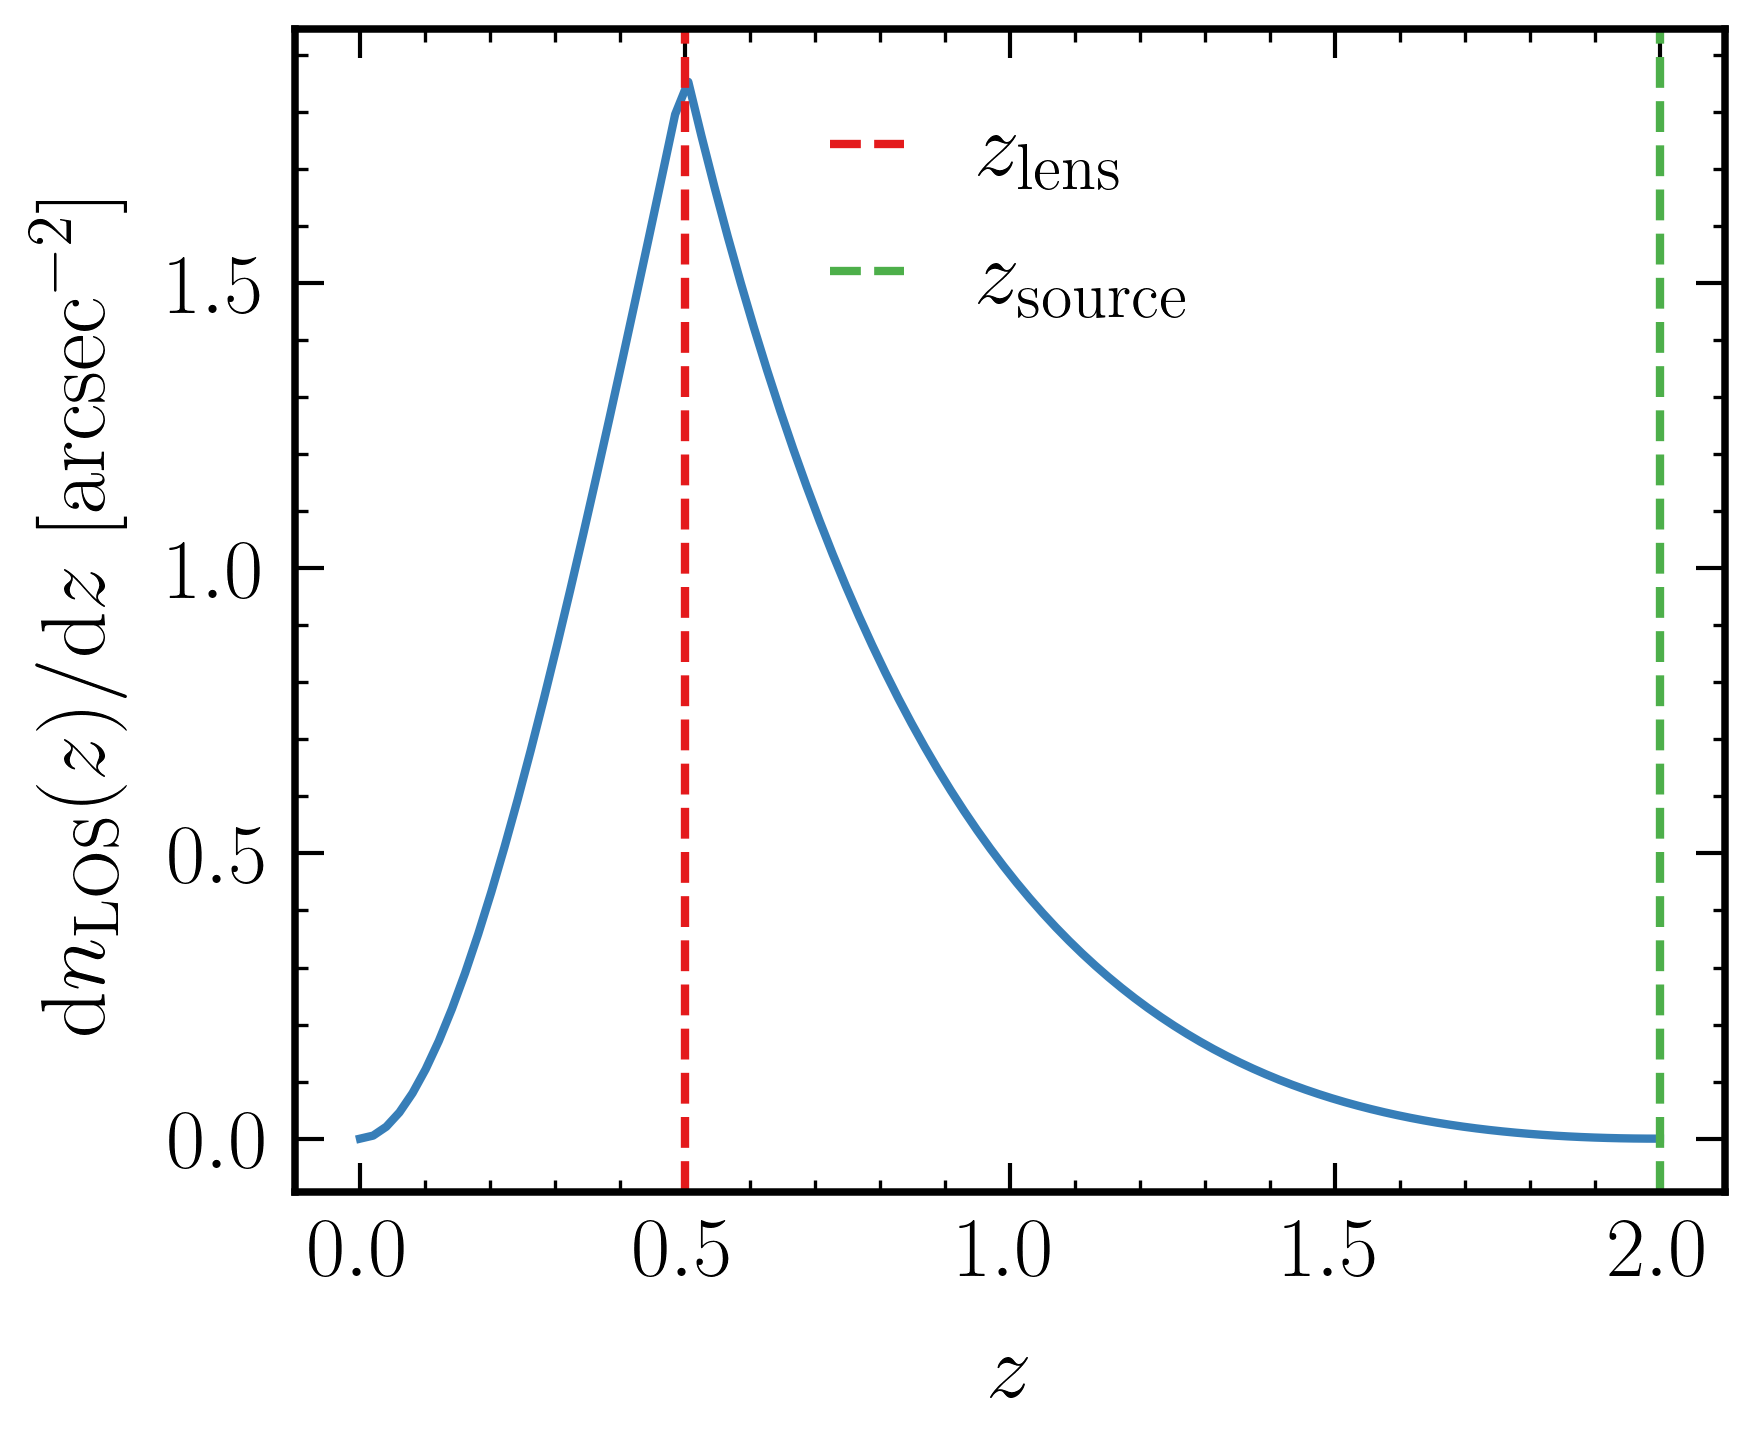
\includegraphics[width=\linewidth]{GL-los-z-dist.png}
	\end{subfigure} 
	\caption{\textit{Left panel:} Convergence map for a \gls*{cdm} subhalo population in the adopted mass range. The convergence map shows how the deflecting mass from all the subhalo lenses is distributed. The full map size is $1 \times 1\ \si{\Mpc}$. We mark in red the virial radius of the main lens halo, in blue its Einstein radius, and in orange the $5 \times 5\ \si{\arcsec}$ lensing image area. \textit{Right panel: }\gls*{los} halos distribution in redshift for our source and lens redshifts configuration, $z_\mathrm{lens}=0.5$ and $z_\mathrm{source}=2$.}
	\label{fig:sl-substructure}
\end{figure}

\Gls*{dm} substructures can be divided into two categories: subhalos that orbit around the main halo at the lens redshift, and \gls*{los} halos distributed between the source and the observer. \Gls*{los} halos are a more direct probe of free-streaming-induced small-scale structure suppression, because they are less affected by baryonic processes and environmental effects, such tidal stripping interactions with the main halo \citep{Despali:2017ksx}. For this reason and the fact that they are expected to be more abundant than subhalos in a lensing system \citep{Despali:2017ksx, He:2021rjd}, it is very important to model them as well, in order to correctly estimate the collective effects of all substructures on the lensing image. 

\subsubsection{Density profile}
To model the density profiles of small-scale \gls*{dm} halos we adopt the smoothly truncated universal 3D mass density profile from \cite{Baltz:2007vq}:
\begin{equation}
    \rho_{\mathrm{tNFW}}(r)= \cfrac{\rho_s}{r/r_s (1+r/r_s)^2}  \cfrac{1}{1+(r/r_t)^2}.
\end{equation}
Here $r$ is the three-dimensional distance from the center of the halo, $\rho_s$ and $r_s$ are respectively the scale density and scale radius that specify a \gls*{nfw} profile \citep{Navarro:1996gj}, and $r_t\equiv\tau r_s$ is the tidal truncation radius that depends on the history of the subhalo. Typical values of the truncation scale $\tau$ range from $4-10$ for spherically symmetric lenses \citep{Gilman:2019nap, Cyr-Racine:2019aa}; we fix $\tau=6$ for simplicity. 
Compared to the standard \gls*{nfw} form, which has an infinite total mass, the truncated \gls*{nfw} contains an additional truncation term that makes the profile decay as $r^{-5}$ for large radii, resulting in a finite total mass given by:
\begin{equation}
    m_\tau=4\pi \rho_s r_s^3 \frac{\tau^2}{(\tau^2+1)^2}[(\tau^2-1)\ln\tau+\tau\pi-(\tau^2 +1)].
\end{equation}
With a fixed truncation scale, the truncated \gls*{nfw} profile is fully determined by the same parameters that determine the \gls*{nfw} profile: the virial mass $m_\mathrm{200, sub}$\footnote{We parameterize subhalos by what would be their mass up to the virial radius $r_{200}$ using the untruncated profile, with the same central density $\rho_s$ and scale radius $r_s$ as the truncated one. This is defined as the mass of the halo enclosed in a sphere where the untruncated halo's average density is 200 times the critical density.} and the concentration $c=r_{200}/r_s$ of the halo. The latter measures how concentrated the mass of a halo is and fixes the density normalization; in principle, it varies from one subhalo to the next and shows dependencies on mass and redshift of the main halo. Here, instead of adopting a concentration-mass relation, we fix $c_{200}=15$ , which is roughly the average value for perturbers in the mass range $10^7-10^{10}\si{\solmass}$ \citep[Fig. 7]{Richings:2020auv}. We anticipate that accounting for scatter in the mass-concentration relation might actually improve our ability to measure subhalos’ parameters as higher concentrations lead to substantially stronger lensing signals \citep{Amorisco:2021iim}.
The equations for calculating the displacement field of a truncated \gls*{nfw} halo, given its mass and position, are fully elaborated by \cite[Appendix A]{Baltz:2007vq}.

To generate perturber populations, we must choose values for their density normalizations and scale radii. Since simulation studies typically measure the halo mass $m_\mathrm{200, sub}$ and the concentration $c$, it is more convenient to sample populations from distributions over these parameters. These variables can then be mapped to the parametrization above via
% The mass in this mapping actually corresponds to $m_{200}$ for an \emph{untruncated} NFW halo!
\begin{align}
    r_s &= \frac{1}{c} \left[ \frac{3 m_\mathrm{200, sub}}{4 \pi \, 200 \rho_\mathrm{cr}(z_\mathrm{lens})} \right]^{1/3} \, ,\\
    \rho_s &= \rho_\mathrm{cr}(z_\mathrm{lens}) \, \frac{1}{3} \frac{c^3}{\log(1+c) - c / (1 + c)} \, . 
\end{align}
For simplicity, we model \gls*{los} halos using exactly the same profile even though they typically have not undergone tidal stripping. 

The parameters of an individual subhalo which are not fixed are thus $\psubb \equiv (x_\mathrm{sub}, y_\mathrm{sub}, m_\mathrm{200, sub})$, where the second and third components are the projected position of the subhalo. In the case of \gls*{los} halos, the parameter set also includes the redshift $z_\mathrm{los}$. In the following sections, we will use arrows to denote vectors, \eg~$\vec{m}_\mathrm{200, sub}$ is an ordered set of masses, one for each simulated subhalo, and bold letters with an arrow to indicate arrays of vectors, \eg~ $\psub \equiv (\bm x_\mathrm{sub}, \bm y_\mathrm{sub}, \bm m_\mathrm{200, sub})$ is an ordered set of mass and positions in the lens plane, one for each simulated subhalo, and equivalently for \gls*{los} halos $\plos \equiv (\bm x_\mathrm{los}, \bm y_\mathrm{{los}}, \bm z_\mathrm{{los}}, \bm m_\mathrm{200, {los}})$. We collectively define the parameters of the full population of perturbers, subhalos and \gls*{los} halos, as $\pp$. In the next two subsections, we describe how we sample these parameters.

\subsubsection{Generating subhalos} \label{subsubsec:sl-model-sub}

We sample subhalo masses from the \gls*{cdm} mass function of \cite{Giocoli:2009ie}:
\begin{equation} \label{eq:shmf}
    \frac{1}{m_\mathrm{200}}\frac{\dd n_\mathrm{sub}( m_\mathrm{200}, z)}{\dd\log m_\mathrm{200}} = A_M (1+z)^{1/2}m_{200}^{\alpha} \exp\left[-\beta\left(\frac{m_\mathrm{200}}{M}\right)^3 \right],
\end{equation}
where $M$ \footnote{
    The total mass of the lens galaxy is described by the Einstein radius of the system, a very well-constrained parameter in lensing inference analyses. For the purpose of describing subhalos, we need to be able to map the measured properties of the lens (the Einstein radius $\theta_\mathrm{E}$) onto the properties of the host halo (the mass $M$). For simplicity, we compute the mass of the host halo transforming the Einstein radius distance measure into a mass measure. We would like to point out a similar approach from \cite{Brehmer:2019jyt}, where they relate the central velocity dispersion of a singular isothermal ellipsoid lens mass distribution profile to the virial mass of the host halo.
}  is the mass of the main lensing halo and $m_\mathrm{200}$ the subhalo mass. The free parameters in this function were fit to hydrodynamical cosmological simulations that included baryons in \cite{Despali:2016meh}. In particular, we use the fits to EAGLE, which give $\alpha = 0.85$ (given in the text) and $(A_M, \beta) = (2.4\times10^{-4}\, \si{\solmass}^{\alpha - 1}, 300)$ (extracted from their figures). The expected number of subhalos in a given mass interval for the lens halo system can be computed by integrating the mass function over that interval.

The spatial distribution of subhalos has been shown to follow an Einasto profile \citep{Springel:2008cc}. However, since the virial radius of a typical main lens halo is much larger than its Einstein radius, and hence, than the image plane, we approximate the distribution to be uniform in the lensing image area. Still, we derive the total number of expected subhalos within the image,  $\bar{n}_\mathrm{sub}$,  via the Einasto fit of \cite{Despali:2016meh}. We find that on average $\bar{n}_\mathrm{sub}=4$ subhalos fall within the lensing image area in our adopted lensing configuration and mass range. %With the lens redshift we have chosen, over a $\SI{5}{\arcsecond} \times \SI{5}{\arcsecond}$ image and integrating over the mass range \SIrange{e7}{e8}{\solmass}, we find $\bar{n}_\mathrm{sub} = 3.1$. 
Thereafter we generate the subhalo population by sampling the number of subhalos from $\operatorname{Poisson}(\bar{n}_\mathrm{sub})$, drawing their masses from the subhalo mass function (Equation~\eqref{eq:shmf}) and sampling their projected positions uniformly over the lens plane. Since the vast majority of subhalos fall outside the lens plane, we expect their lensing effect to be mostly degenerate with external shear, and thus do not simulate them. In the left panel of Figure~\ref{fig:sl-substructure} we show the convergence map for one realization of our subhalo population.

\subsubsection{Generating line-of-sight halos}

As described in \cite[Figure 3]{CaganSengul:2020nat}, we first compute the average number of \gls*{los} halos in the double-pyramid geometry connecting the observer, lens-plane and source. For each simulation we sample the number of \gls*{los} halos from $\operatorname{Poisson}(\bar{n}_\mathrm{los})$. We then sample their redshifts and projected positions uniformly over the double-pyramid region and draw their masses from the mass function in \cite{Tinker:2008ff}, assuming an overdensity with respect to the critical density of the universe at the epoch of analysis of $\Delta=200$. 

More in details, we infer the number of detectable \gls*{los} halos by integrating their mass function in the mass range adopted for the analysis and within the double-cone volume
\begin{equation}
    \bar{n}_{\mathrm{los}}=\int_0^{z_\mathrm{src}}\int_{m_\mathrm{200,min}}^{m_\mathrm{200, max}} n_\mathrm{los}(m_\mathrm{200}, z)\dd{m_\mathrm{200}} \frac{\dd{V}}{\dd{z}}\dd z.
\end{equation}
On average we get $\bar{n}_{\mathrm{los}}=260$ \gls*{los} halos projected in our lens plane. Similarly to what we do with the subhalo population, when generating simulated images, we draw the number of LOS halos from $\operatorname{Poisson}(\bar{n}_\mathrm{los})$, we then sample their masses and redshift from the \cite{Tinker:2008ff} halo mass function and sample their projected positions uniformly over the lensing image area. As with subhalos, we ignore any \gls*{los} halos lying outside the double pyramid volume. In right panel of Figure~\ref{fig:sl-substructure} we show the distribution of \gls*{los} halos in redshift for our lens and source redshifts configuration.

To avoid expensive iterative ray-tracing through the lens planes of each \gls*{los} halo, we project them as effective subhalos into the lens plane, using the relations derived in \cite{CaganSengul:2020nat} to rescale their scale radii and masses. Following \cite{CaganSengul:2020nat}, \gls*{los} halos at comoving distance $\chi$ can be treated as subhalos on the main-lens plane with an effective projected mass density given by:
\begin{equation}
    \Sigma_{\chi, \mathrm{eff}}(D_L\vec{x};m_{200},r_s,\tau)= \Sigma(D_L\vec{x};m_{200,\mathrm{eff}},r_{s,\mathrm{eff}},\tau).
\end{equation}
The effective scale radius $r_{s,\mathrm{eff}}$ and mass $m_{200,\mathrm{eff}}$ are respectively
\begin{equation}
    r_{s,\mathrm{eff}}=\cfrac{D_L}{g(\chi)D_\chi}r_s,
\end{equation}
and
\begin{equation}
    m_{200,\mathrm{eff}}=f(\chi)\cfrac{\Sigma_{\mathrm{cr}, l}}{\Sigma_{\mathrm{cr}, \chi}}\left(\cfrac{D_l}{g(\chi)D_\chi}\right)^2m_{200}.
\end{equation}
The piecewise functions $f(\chi)$ and $g(\chi)$ are:
\begin{equation}
    f(\chi)= \begin{cases}
            1-\beta_{\chi l} & \chi \leq \chi_L \\
            1-\beta_{l\chi}  & \chi > \chi_L \\
            \end{cases},
\end{equation}
and
\begin{equation}
    g(\chi)= \begin{cases}
            1 & \chi \leq \chi_L \\
            1-\beta_{l\chi}  & \chi > \chi_L \\
            \end{cases},
\end{equation}
with $\beta_{ij}=\cfrac{D_{ij}D_s}{D_jD_{is}}$, where $D_i$ is the angular diameter distance from the observer to plane i, and $D_{ij}$ is the angular diameter distance from lens plane i to lens plane j, and $\chi_L$ is the comoving distance to the main-lens plane.
We have also introduced the critical surface density at plane i
\begin{equation}
    \Sigma_{\mathrm{cr}, i}\equiv \cfrac{c^2D_s}{4\pi G D_i D_{is}}.
\end{equation}

It should be noted that effective convergence methods, like the one we adopt \citep{CaganSengul:2020nat}, do not fully capture the subtleties and degeneracies of multi-plane lens analysis, by disregarding how, when a \gls*{dm} small-scale halo is not in the lens plane, the lens mass model can absorb its lensing signal \citep{Fleury:2021tke, Amorisco:2021iim, He:2021rjd}. The omission of this effect may lead to an overestimate of the \gls*{los} halos contribution and needs to be addressed before this technique can be safely used for the analysis of real data.

For \gls*{los} halos we adopt the same concentration and truncation scale values used for subhalos.


\subsection{Modelling free-streaming effects in WDM}
\label{subsec:free-streaming}

\begin{figure}
    \centering
    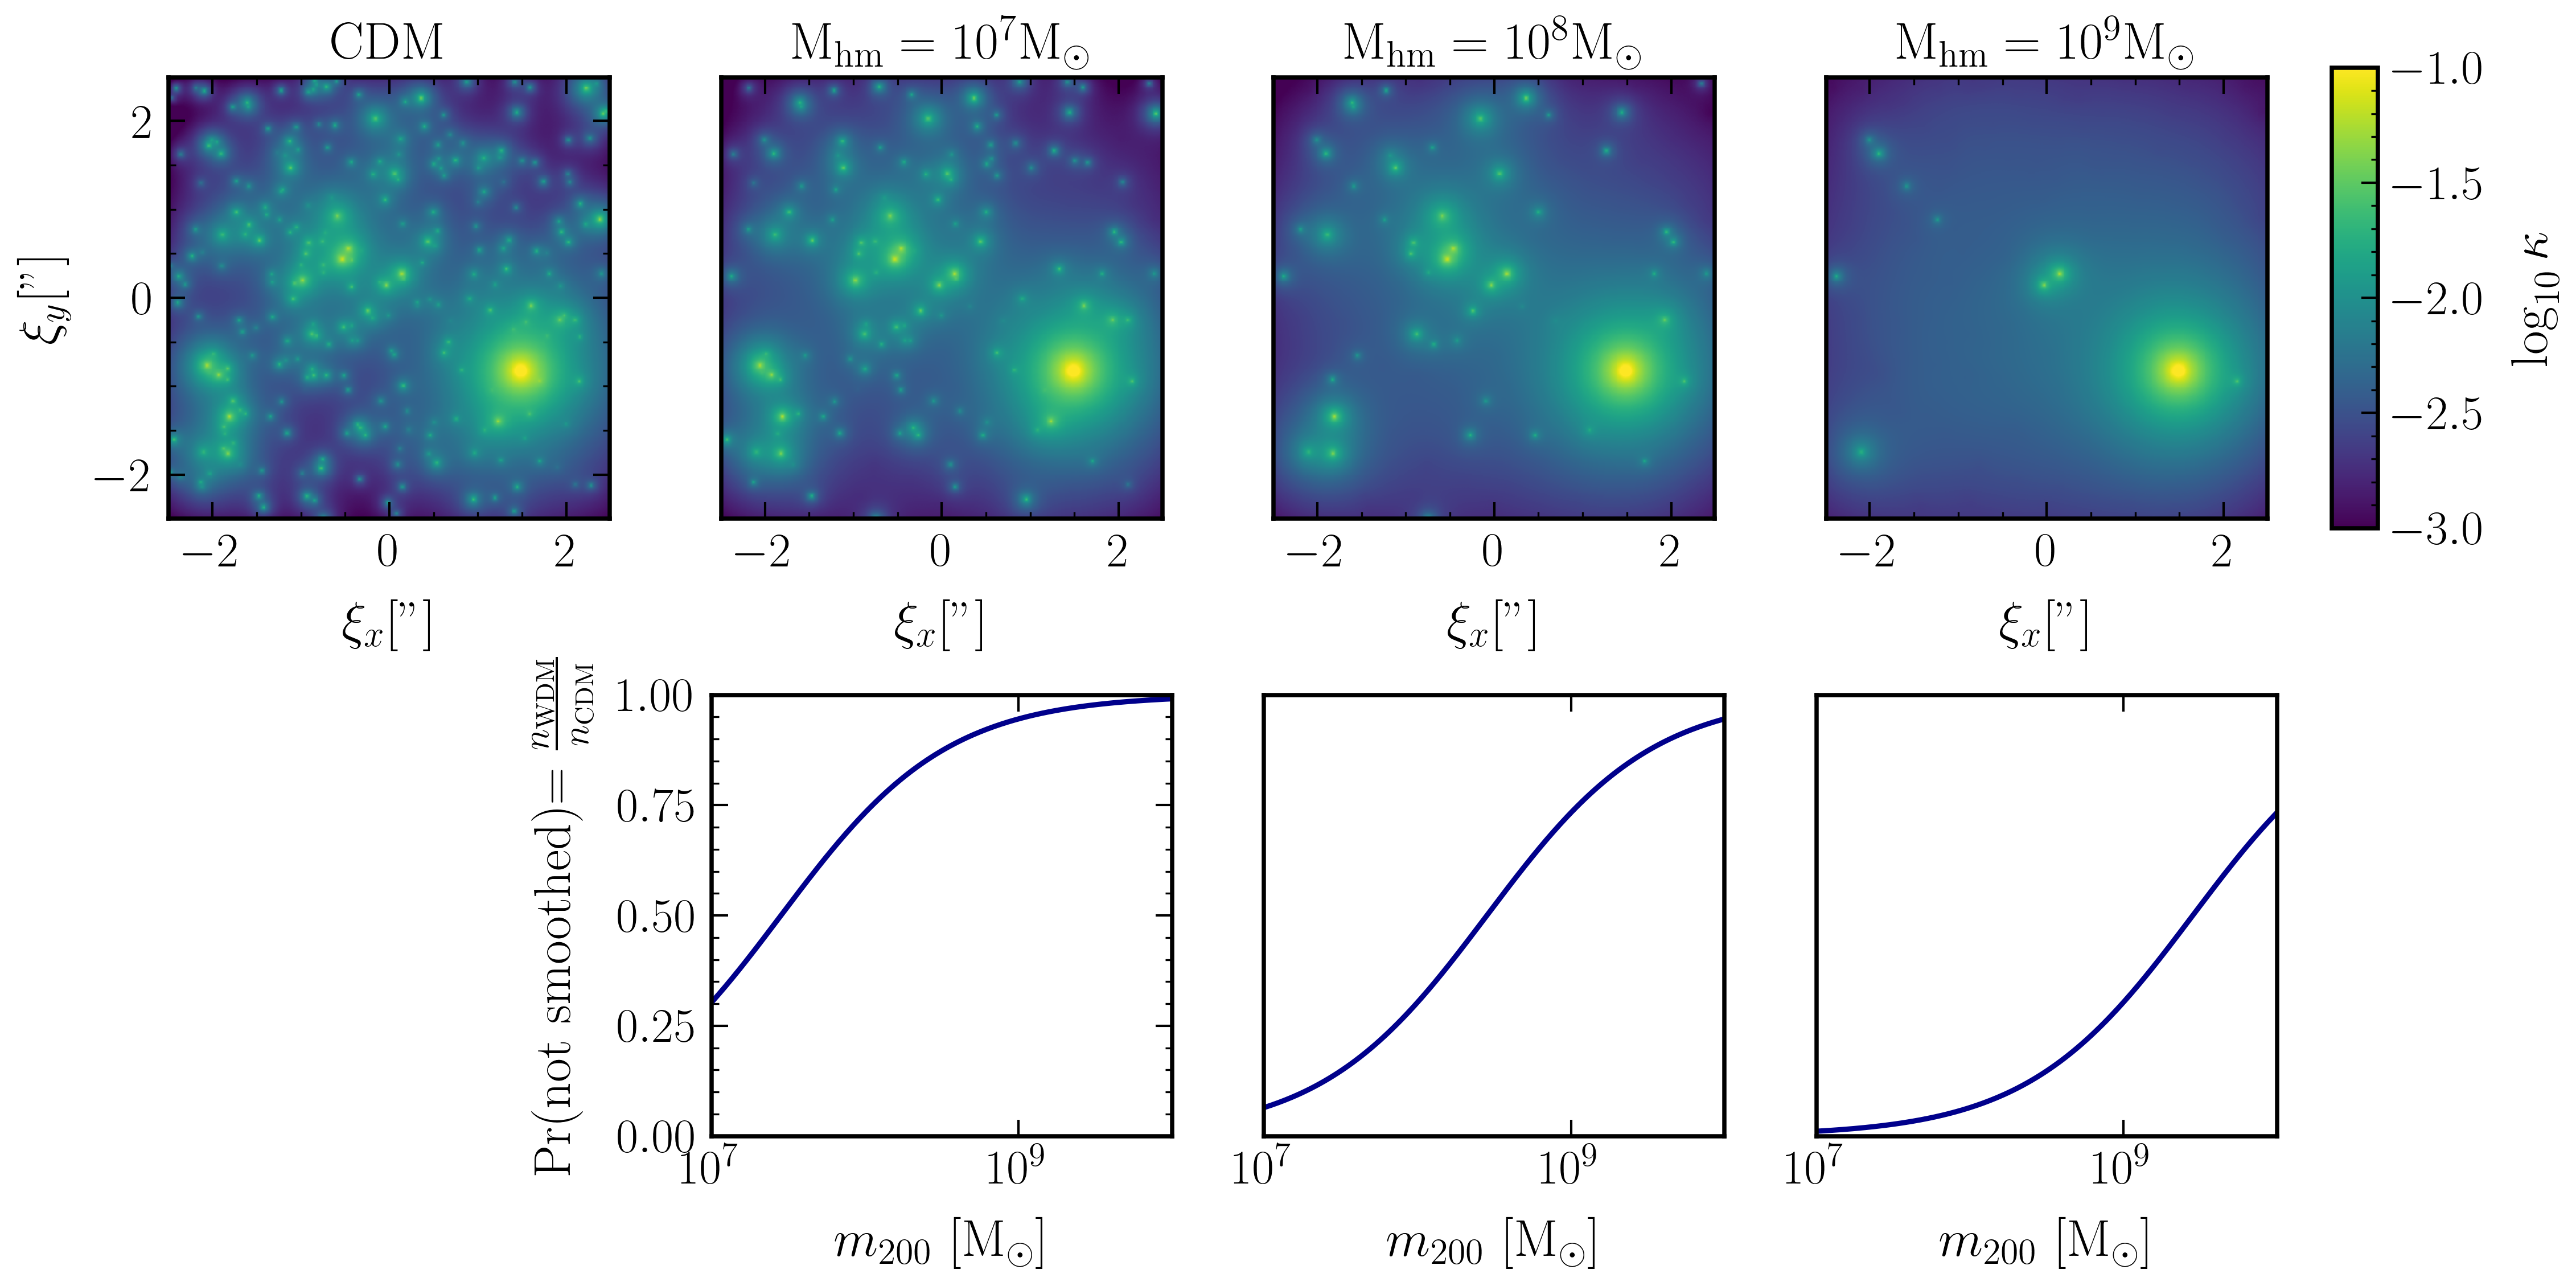
\includegraphics[width=\linewidth]{GL-smoothing.png}
    \caption{
    \textit{Top}: Convergence maps for a population of \gls*{los} halos with masses sampled from the \gls*{cdm} \gls*{hmf} in the adopted mass range (Table~\ref{tab:model}) and projected in the lens plane following the prescription from \cite{CaganSengul:2020nat}.
    In the second to fourth columns, we imitate the effect of WDM with different cutoff masses (as labeled in the titles) via our smoothing scheme. \textit{Bottom}: We show the probability with which \gls*{los} halos do not get smoothed, equal to the ratio between the WDM and the CDM HMF (Equation~\eqref{eq:cutoff}). The smoothing is stochastic, so for each realization of the smoothing different halos are smoothed.
    }
    \label{fig:smoothing}
\end{figure}

Among \gls*{dm} models, \gls*{wdm} particle candidates, sterile neutrinos \citep{Boyarsky:2018tvu} and gravitinos \citep{Bond:1982uy}, are well-motivated from a particle physics perspective. In \gls*{wdm} models \gls*{dm} particles have non-negligible thermal velocities that allow them to free-stream out of density perturbations, effectively preventing small-scale structure formation. The suppression scale at which this happens depends on model parameters and is parametrised by the half-mode mass $\mhm$ in the \gls*{hmf}. Therefore, one of the viable way to discriminate between \gls*{cdm} and alternative \gls*{wdm} models is to constrain the low-mass end of the \gls*{hmf} by measuring the half-mode mass $\mhm$ . 

The free-streaming effects of \gls*{wdm} are well described in terms of the half-mode wavelength $\lambda_{\mathrm{hm}}$, which corresponds to the scale at which the \gls*{dm} transfer function falls to half the \gls*{cdm} transfer function. We can define the half-mode mass as the mass contained within a radius of the half-mode wavelength:
\begin{equation}
\mhm=\frac{4\pi\Omega_{\mathrm{M}}\rho_{\mathrm{crit}}}{3}\left(\frac{\lambda_{\mathrm{hm}}}{2}\right)^3,
\end{equation}
where $\Omega_{\mathrm{M}}$ is the matter density parameter and $\rho_{\mathrm{crit}}$ is the critical density of the universe.
Following \cite{Schneider:2011yu}, the half-mode wavelength,
\begin{equation}
    \lambda_{\mathrm{hm}}=2\pi\alpha_{\mathrm{hm}}\left(2^{\nu/5}-1\right)^{-1/(2\nu)},
\end{equation}    
is the scale below which the initial density perturbations are completely erased, with $\nu= 1.12$ and, assuming that all \gls*{dm} is warm,
\begin{equation}
\alpha_{\mathrm{hm}}=0.049\left(\frac{m_\mathrm{WDM}}{\si{\keV}}\right)^{-1.11}\left(\frac{\Omega_\mathrm{DM}}{0.025}\right)^{0.11}\left(\frac{h}{0.7}\right)^{1.22}h^{-1}\si{\Mpc}.
\end{equation}

We then have a one-to-one mapping between the mass of the \gls*{wdm} particle and the half-mode mass.
For strong lensing, the half-mode mass can be thought of as an effective cutoff mass below which the \gls*{dm} mass function is strongly suppressed. To model this suppression in the \gls*{wdm} mass function we adopt for both subhalos and \gls*{los} halos the functional form from \cite{Lovell:2020bcy}:
\begin{equation}\label{eq:cutoff}
    \frac{n_{\mathrm{WDM}}}{n_{\mathrm{CDM}}}=\left(1+\left(\alpha\frac{\mhm}{m_{200}}\right)^\beta\right)^\gamma,
\end{equation}
with best fit parameters $\alpha=4.2$, $\beta=2.5$, and $\gamma=0.2$ for subhalos, $\alpha=2.3$, $\beta=0.8$, and $\gamma=1$ for central halos.

\subsubsection{Smoothing substructures}
\label{subsubsec:smoothing}

The observational signature of \gls*{wdm} is, thus, the absence of small-scale structures. However, in the current parameterization, this is accompanied by the removal of the corresponding mass enclosed in them, whereas in reality the mass will still be present but will be diffused throughout the smooth main halo. This effect is manifested in a correlation between the half-mode mass and the main-halo Einstein radius: suppressing more substructure leads to an increase in the inferred Einstein radius since the total mass of the system (within the image) is tightly constrained by the size of the observed ring (or arcs).

We introduce a prescription for dealing with this degeneracy, which well captures the physical reality of structure suppression due to free streaming. 
Halos that should be suppressed are not present because the \gls*{dm} particles that should make them up are freely streaming, and their mass is therefore more diluted throughout the main halo.
Therefore, rather than removing or adding substructures as a response to a changing cutoff, we still sample substructures from the \gls*{cdm} mass function, but we smooth the displacement field generated by halos that should be suppressed based on the aforementioned prescription by \cite{Lovell:2020bcy} to hide their lensing signature. In other words, each sampled small-scale halo has a probability equal to the ratio between the \gls*{wdm} and the \gls*{cdm} \gls*{hmf} (Equation~\eqref{eq:cutoff}) of not being smoothed. 

We then effect the smoothing by convolving the deflection field of each individual sub-/\gls*{los} halo with a radially-symmetric filter
\begin{equation}
f \propto 1 - \exp\left(-\left(\frac{r}{r_{\mathrm{smooth}}}\right)^{n_{\mathrm{smooth}}}\right).
\end{equation}
This filtering preserves the far-field lensing signature of the halo, which is only determined by its total mass.
By default, we choose the smoothing scale to be equal to the halo virial radius: $r_\mathrm{smooth}=r_{200}$, and the smoothing exponent $n_\mathrm{smooth}=2$.

In the top row of Figure~\ref{fig:smoothing} we visualize the convergence maps in the lens plane for the same realization of \gls*{los} halos drawn from \gls*{cdm} distributions (panel 1), and with different cutoff masses implemented with our smoothing scheme (panels 2-4). In the bottom row, we show how we decide to smooth the lensing signature of certain halos based on the ratio between the \gls*{wdm} and the \gls*{cdm} \gls*{hmf} (Equation~\eqref{eq:cutoff}). 


\subsection{Instrumental effects}

We generate mock data with comparable quality to \gls*{hst} observations. All images are $\SI{5}{\arcsecond} \times \SI{5}{\arcsecond}$ with $\SI{0.05}{\arcsecond}$ resolution ($100 \times 100$ pixels). In our simulations, we do not include a \gls*{psf} for simplicity, but this component cannot be disregarded in real data analysis. To account for the fact that each pixel in the image corresponds to a finite collecting region in the sky, we generate our images at a resolution eight times higher than the target resolution and downsample. In experiments we found that neglecting this effect can have a significant impact on inference results. Lastly, we add Gaussian and uncorrelated pixel noise to our observations such that the brightest pixels are approximately 30 times the noise level (after downsampling), representative of \gls*{hst} data.



\section{Methodology}

\section{Measuring single subhalo parameters} \label{sec:results-sub}

\subsection{Mock data generation}
\label{subsec:sub-data}

Table~\ref{tab:params-and-priors}
%We want our simulations to be representative of \gls*{hst} data, in order to demonstrate that our pipeline is in principle able to extract the signal of interest from them. We adopt a pixel scale of \SI{0.05}{\arcsecond}, being slightly larger than the expected \SI{0.04}{\arcsecond}, which allows us to disregard its \gls*{psf} \citep{Gennaro:2018aa} for simplicity. The size of the images is $100 \times 100$ pixels, so they cover an area of $5 \times 5\ \si{\arcsecond}$ on the sky. 
%Initially, we generate the mock data with a resolution 10-times higher and then downsample it to the adopted resolution by local averaging, effectively simulating integration of the light across the pixel areas.
%
%We model the instrumental effects by simply assuming a Gaussian and uncorrelated pixel noise. The noise level $\sigma$ is set so that the peak \gls*{snr} ratio of the image is $\num{\sim 30}$ (after downsampling), representative of \gls*{hst} data. Then, given a modeled flux, our simulator is given by:
%\begin{equation}
%    p(\data\mid\psrc, \plens,\pp, \vartheta)
%    = \mathcal{N}(\data\mid\mathrm{obs}(\psrc, \plens, \pp, \vartheta), \sigma^2).
%\end{equation}
%We leave to future works to account for the correct modeling of the \gls*{psf} and correlated pixel noise, which are fundamental in order to correctly conduct substructure studies in strong gravitational lensing images.
%
%In Figure~\ref{fig:mock} we show a gallery of twenty mock strong-lensing images we use as target observations. These mock observations have been generated with arbitrary lens and source parameters drawn from the initial prior in Table~\ref{tab:model}. Their peak \gls*{snr} is $\num{\sim 30}$, representative of \gls*{hst} data.

\subsection{Inference strategy}
\label{subsec:sub-nn}


\todo{Rephrase}
We now apply \gls*{tmnre} to three different substructure lensing problems of increasing complexity. For all tasks we use the same general ratio estimator architecture. It consists of an initial compression network that maps the $100 \times 100$ pixel images into a feature vector. This feature vector is concatenated to $\psub$ (and separately to $\psrc$ and $\plens$ for tasks where they are also inferred). The vector is then passed to a \gls*{mlp} which outputs an estimate of the 2D and 1D marginal likelihood-to-evidence ratios for $(x_\mathrm{sub}, y_\mathrm{sub})$ and $\log_{10} m_\mathrm{sub} / \si{\solmass}$ respectively (with separate \gls*{mlp}s used to estimate the 1D ratios for $\psrc$ and $\plens$).

For each ratio estimator we begin the first training round with \num{10000} training examples. We then truncate each parameter's prior. If none of the truncated priors shrank by at least 20\%, we increase the number of training examples by a factor of \num{1.5} for the next inference round. A fresh network is then trained using simulations drawn from the truncated prior. Convergence of the ratio estimator is declared after five such consecutive increases in the training set size. For tasks in which we must infer the macromodel parameters we first train the macromodel ratio estimator using this procedure and use the resulting truncated priors to generate training data for the subhalo ratio estimators using the same training procedure. We use the implementation of \gls*{tmnre} in \texttt{swyft}\footnote{
    \url{https://github.com/undark-lab/swyft/}
} \citep{Miller:2022shs}, which is built on \texttt{PyTorch} and \texttt{pytorch-lightning}\footnote{
    \url{https://www.pytorchlightning.ai/}
}.

The training data for our ratio estimators differs in important ways from typical datasets studied by machine learning researchers, making the choice of a good compression network an interesting challenge. Consider, for example, the machine learning problem of classifying the content of natural images. Natural images are distinguished by a hierarchy of visual features at different scales (for example, small-scale features such as textures and edges which comprise large-scale features like the head of an animal or part of an object). A good image classifier should be translation-invariant, producing the same output regardless of the position of an image's contents. Since the deep \gls*{cnn} architecture has an inductive bias towards learning a hierarchy of features and are translation invariant, \gls*{cnn}s are widely used in computer vision.

The training data for our ratio estimators does not share these features. Different perturber configurations produce images with slightly different relationships between the multiple images of the source galaxy. The variations between images lie near the Einstein ring, and do not show the same rich hierarchical structure of natural images. This means that inductive biases of \gls*{cnn}s are not necessarily beneficial in the context of substructure lensing.

In our experiments, we used \gls*{cnn}s in the ratio estimators for the macromodel parameters, finding their performance to be adequate. However, we found they produced much too wide 2D marginals for the position of a subhalo. Instead, we found the MLP Mixer \citep{Tolstikhin:2021aa} to work well.\footnote{
    The MLP Mixer implementation we use can be found at \url{https://github.com/lucidrains/mlp-mixer-pytorch}.
} Roughly, the MLP Mixer splits the image into patches, stacks the patches and passes each pixel in the stack through an \gls*{mlp}, acting as a dilated convolution. Another MLP is then applied along the channel dimension of the mixed patches, and the process is iterated. The MLP Mixer thus directly examines the relationships between pixels in disparate parts of the image, which is exactly how the properties of subhalos are imprinted. We expect that other architectures that split the image into patches such as \gls*{vit} \citep{Dosovitskiy:2020qjv} could work well for the compression network, though \gls*{vit} is known to require large amounts of training data.

The architectures of our macromodel and subhalo compression networks are given in \autoref{app:architectures}. While we did not perform a full hyperparameter exploration, we found the batchnorm layers to be crucial for stable training of the \gls*{cnn} used for the macromodel ratio estimator. Since our images are roughly one-quarter the area of the images studied in the paper introducing MLP Mixer, we use a substantially smaller model than they suggest. Using dropout in the MLP Mixer and classifier \gls*{mlp}s improved performance. Varying the number of hidden layers and their size in the classifiers had little impact.

We used the Adam optimizer with an initial learning rate of \num{6e-3} for the macromodel ratio estimator and \num{4e-4} for the subhalo ratio estimator (found through a learning rate test) and a batch size of \num{64}. The learning rate was reduced by a factor of \num{0.1} whenever the validation loss plateaued for \num{3} epochs. Training was run for no longer than \num{30} epochs.

\begin{table}
    \centering
    \begin{tabular}{c c c c c}
        \toprule
        & Parameter & True value & Initial prior & First inferred in \\
        \midrule
        \parbox[t]{1mm}{\multirow{3}{*}{\rotatebox[origin=c]{90}{Subhalo}}}
        & $x_\mathrm{sub}\, ['']$ & \num{-1.1} & $\Uniform(-2.5, 2.5)$ & Section~\ref{subsec:sp} \\
        & $y_\mathrm{sub}\, ['']$ & \num{-1.1} & $\Uniform(-2.5, 2.5)$ & Section~\ref{subsec:sp} \\
        & $\log_{10} m_\mathrm{sub}/\si{\solmass}$ & \num{9.5} & $\Uniform(8, 10.5)$ & Section~\ref{subsec:lss}\\
        % & $n_\mathrm{sub}$ & ? & $\operatorname{Poisson}(?)$ \\
        \midrule
        \parbox[t]{1mm}{\multirow{6}{*}{\rotatebox[origin=c]{90}{SPLE}}}
        & $x_\mathrm{lens}\, ['']$ & -0.05 & $\Uniform(-0.2, 0.2)$ & \multirow{6}{*}{Section~\ref{subsec:lss}} \\
        & $y_\mathrm{lens}\, ['']$ & 0.1 & $\Uniform(-0.2, 0.2)$ \\
        & $\varphi_\mathrm{lens} \, [^\circ]$ & 1 & $\Uniform(0.5, 1.5)$ \\
        & $q_\mathrm{lens}$ & 0.75 & $\Uniform(0.5, 1)$ \\
        & $\gamma$ & 2.1 & --- \\
        & $r_\mathrm{ein}\, ['']$ & 1.5 & $\Uniform(1, 2)$ \\
        \midrule
        \parbox[t]{1mm}{\multirow{2}{*}{\rotatebox[origin=c]{90}{Shear}}}
        & $\gamma_1$ & 0.005 & $\Uniform(-0.5, 0.5)$ & \multirow{2}{*}{Section~\ref{subsec:lss}} \\
        & $\gamma_2$ & -0.010 & $\Uniform(-0.5, 0.5)$ \\
        \midrule
        \parbox[t]{1mm}{\multirow{7}{*}{\rotatebox[origin=c]{90}{Source}}}
        & $x_\mathrm{src}\, ['']$ & 0 & $\Uniform(-0.2, 0.2)$ & \multirow{7}{*}{Section~\ref{subsec:lss}} \\
        & $y_\mathrm{src}\, ['']$ & 0 & $\Uniform(-0.2, 0.2)$ \\
        & $\varphi_\mathrm{src} \, [^\circ]$ & 0.75 & $\Uniform(0.5, 1.25)$ \\
        & $q_\mathrm{src}$ & 0.5 & $\Uniform(0.2, 0.8)$ \\
        & $n$ & 2.3 & $\Uniform(1.5, 3)$ \\
        & $r_e\, ['']$ & 2.0 & $\Uniform(0.5, 3)$ \\
        & $I_e$ & 0.6 & $\Uniform(0.1, 2)$ \\
        \bottomrule
    \end{tabular}
    \caption{True subhalo and macromodel parameter values and priors used in the first \gls*{tmnre} inference round in our three inference tasks. The last column references the first section in which the indicated parameter is inferred rather than being fixed to its true value. The slope of the main lens is fixed to \num{2.1}, as explained in Section~\ref{subsec:sl-model-lens}. The main lens and source redshifts are set to $z_\mathrm{lens} = 0.5$ and $z_\mathrm{src} = 2$ respectively. For the analysis in Section~\ref{sec:lshs} involving a population of light perturbers, we sample the number of \gls*{los} and subhalos from Poisson distributions with means $\bar{n}_\mathrm{los} = 265.6$ and $\bar{n}_\mathrm{sub} = 3.1$ respectively, and restrict their masses to the range $10^7-10^8\si{\solmass}$. The halo mass functions and redshift distributions are described in detail in Section~\ref{subsec:substructure}. For all perturbers we fix the concentration to $c = 15$ and truncation scale $\tau = r_t / r_s = 6$.}
    \label{tab:params-and-priors}
\end{table}

\subsection{Subhalo position inference with fixed mass, source and lens}\label{subsec:sp}

We first consider the case where the only free parameters in the lens are the position of a single $10^9\si{\solmass}$ subhalo, $\psubb = (x_\mathrm{sub}, y_\mathrm{sub})$. The prior is taken to be uniform over the image plane (\ie, $\Uniform(-2.5, 2.5)$ for both coordinates). The posterior for $\psubb$ can then be computed analytically. Adopting a uniform prior over $\psubb$ covering the image plane and using the fact the posterior is much narrower, we have
\begin{equation}
    \log p(\psubb \mid \data) % &= \log \normal(\data \mid \bm{f}(\psub), \sigma_n^2) \\
    \sim -\frac{1}{2} \sum_{i,j} \left( \frac{x_{ij} - f_{ij}(\psubb)}{\sigma_n} \right)^2 \, ,
\end{equation}
where the sum runs over pixels and we dropped terms independent of $\psubb$.

\begin{figure}
    \centering
    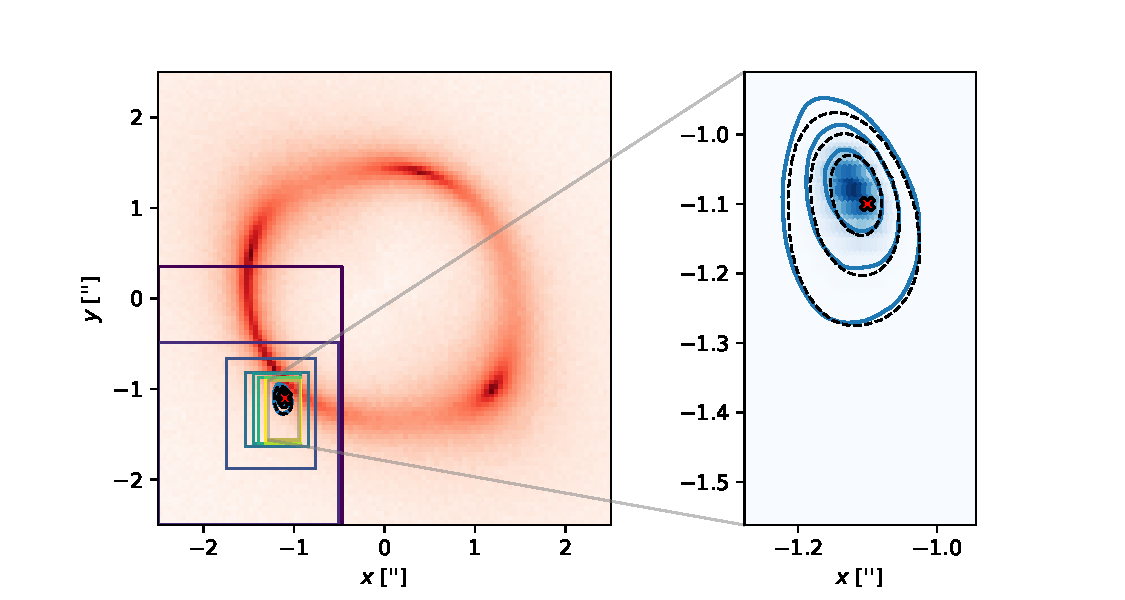
\includegraphics[height=5cm]{GL-sp-post-2d.pdf}
    \caption{Validation of \gls*{tmnre} through inference of the position of a subhalo, with macromodel parameters fixed to their true values and the subhalo's mass fixed to $10^9\si{\solmass}$. The observation is shown in the left panel. The blue and dashed black contours correspond to the posterior inferred with \gls*{tmnre} and computed analytically respectively, indicating the 68\%, 95\% and 99.7\% credible regions. The red {\color{red} $\times$} shows the subhalo's true position. The blue through yellow boxes in the left panel show the ranges of the truncated prior based on the 1D marginals for the subhalo's coordinates. The zoom-in on the right encompasses the range of the final truncated prior. The distorted blue hex-bin histogram shows the magnitude of the inferred posterior.}
    \label{fig:gl-sp-post}
\end{figure}

\begin{figure}
    \centering
    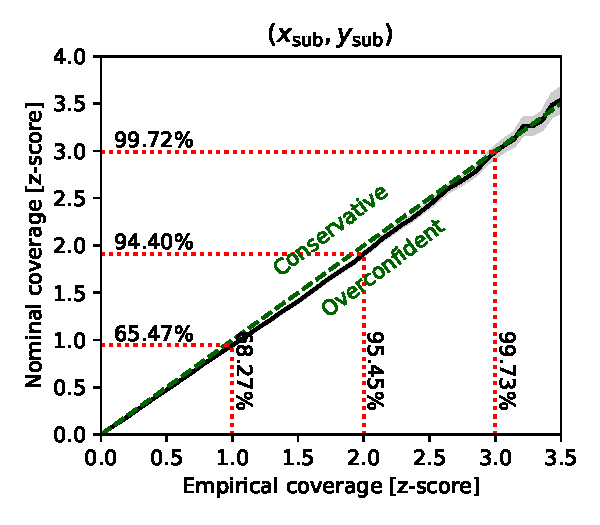
\includegraphics[height=5cm]{GL-sp-coverage-2d.pdf}
    \caption{Coverage plot for inference task where only the subhalo's position is free (see Figure~\ref{fig:gl-sp-post}), showing our ratio estimator produces posteriors of the correct size on average. In detail, the black curve shows the empirical versus nominal coverage, estimated by computing posteriors for \num{10000} observations drawn from the final truncated prior. The statistical uncertainty of this estimate is plotted in grey; its derivation is explained in detail in \cite{Cole:2021gwr}. For a perfectly-calibrated ratio estimator, the black curve would lie along the diagonal green dashed line. The red dashed lines indicate the empirical and nominal coverage of the $1 - 3 \sigma$ credible regions.}
    \label{fig:gl-sp-coverage}
\end{figure}

Figure~\ref{fig:gl-sp-post} shows the truncation regions for each round and compares the analytically-computed posterior with the posterior inferred using \gls*{tmnre}. While the truncation regions and posterior estimates in early rounds are extremely broad compared to the analytically-computed posterior, \gls*{tmnre} successfully identifies the region of the image containing the subhalo. After 10 inference rounds the truncation region stabilizes and the inferred posteriors agree well with the true ones for each coordinate. To complement this visual check we also check the coverage for samples from the final round of \gls*{tmnre} in Figure~\ref{fig:gl-sp-coverage}. We find the empirical and nominal coverage to be in good agreement, with our ratio estimator very slightly underestimating the width of the posterior beyond the 95\% confidence level.

Having validated \gls*{tmnre} in this simple scenario, we now turn to more complex inference tasks where the posteriors of interest cannot be derived analytically.

\subsection{Subhalo mass and position inference}\label{subsec:lss}

Next we aim to infer the position and mass of a single subhalo, $\psubb = (m_\mathrm{sub}, x_\mathrm{sub}, y_\mathrm{sub})$, in a system where the source and main lens parameters are also unknown. The priors for the \num{17} parameters of the model are given in Table~\ref{tab:params-and-priors}. Due to the relatively low dimensionality, inference on this model is within the reach of likelihood-based tools such as \gls*{mcmc} or nested sampling. In addition, it can be implemented in a differentiable manner, making the application of methods such as \gls*{hmc} possible \citep{Gu:2022xhk,Chianese:2019ifk}. Running such expensive scans is beyond the scope of this paper.

The final posteriors for the subhalo parameters are shown in Figure~\ref{fig:gl-lss-sub-post}. The true values of all parameters fall within the $\sim 68\%$ credible intervals of the inferred posteriors. We find the effect of the uncertain macromodel is not too strong (at least for this noise realization), with the size of the subhalo position posterior being comparable to what we found in the previous inference task.
% Due to the uncertainties in the source, lens and subhalo mass the posteriors are slightly wider than for the previous inference task. The subhalo's parameters are also not measured accurately enough to truncate their priors, even in the final inference round. 
Figure~\ref{fig:gl-lss-sub-coverage} demonstrates that our ratio estimator has good coverage with respect to the constrained prior. In Figure~\ref{fig:gl-lss-macro-post} and Figure~\ref{fig:gl-lss-macro-coverage} we display the marginal posteriors and coverage plots for all 14 source and main lens parameters, which demonstrate they are well-calibrated.

\begin{figure*}
    \centering
    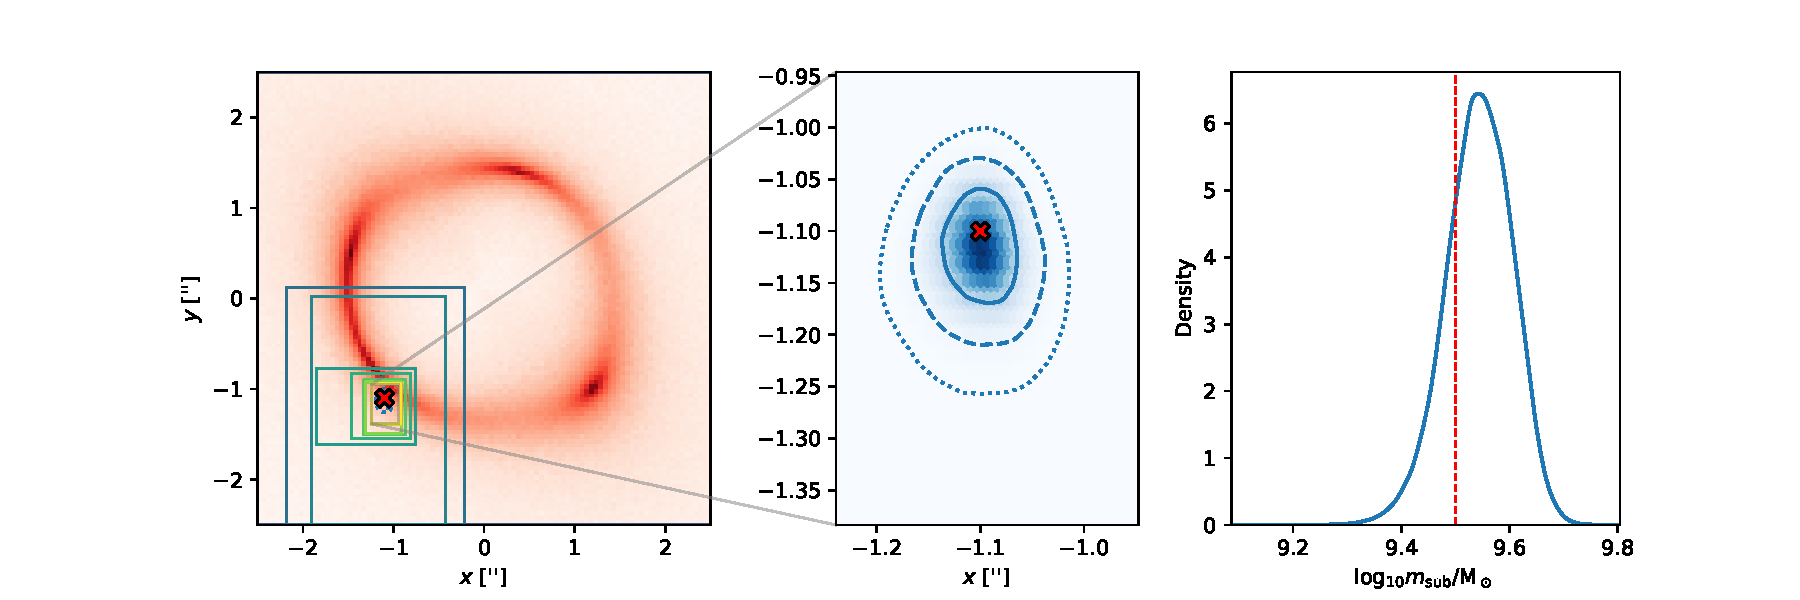
\includegraphics[width=\textwidth]{GL-lss-post-2d.pdf} %height=6cm
    \caption{Marginal posteriors inferred with \gls*{tmnre} for a subhalo's 2D position (left and center) and mass (right) in a lens with unknown macromodel parameters. See the caption of Figure~\ref{fig:gl-sp-post} for further details, though note we have instead used solid, dashed and dotted lines respectively to mark the 68\%, 95\% and 99.7\% credible regions of the position posterior. The range of the $x$-axis in the right panel shows the final-round truncated prior for the subhalo's $\log_{10}$-mass.}
    \label{fig:gl-lss-sub-post}
\end{figure*}

\begin{figure*}
    \centering
    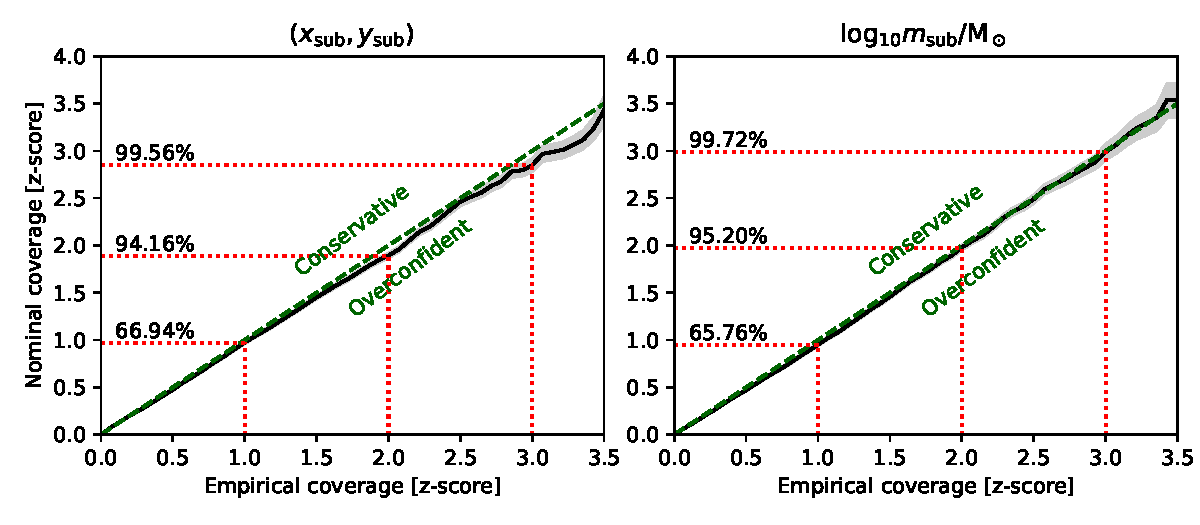
\includegraphics[width=0.84\linewidth]{GL-lss-sub-coverage-2d.pdf}
    \caption{Coverage plots for subhalo position and mass ratio estimators learned from the observation in Figure~\ref{fig:gl-lss-sub-post}. These again indicate the estimators' credible regions are on average the correct size for observations drawn from the final-round truncated prior. See Figure~\ref{fig:gl-sp-coverage} for an explanation of the format.}
    \label{fig:gl-lss-sub-coverage}
\end{figure*}

\begin{figure*}
    \centering
    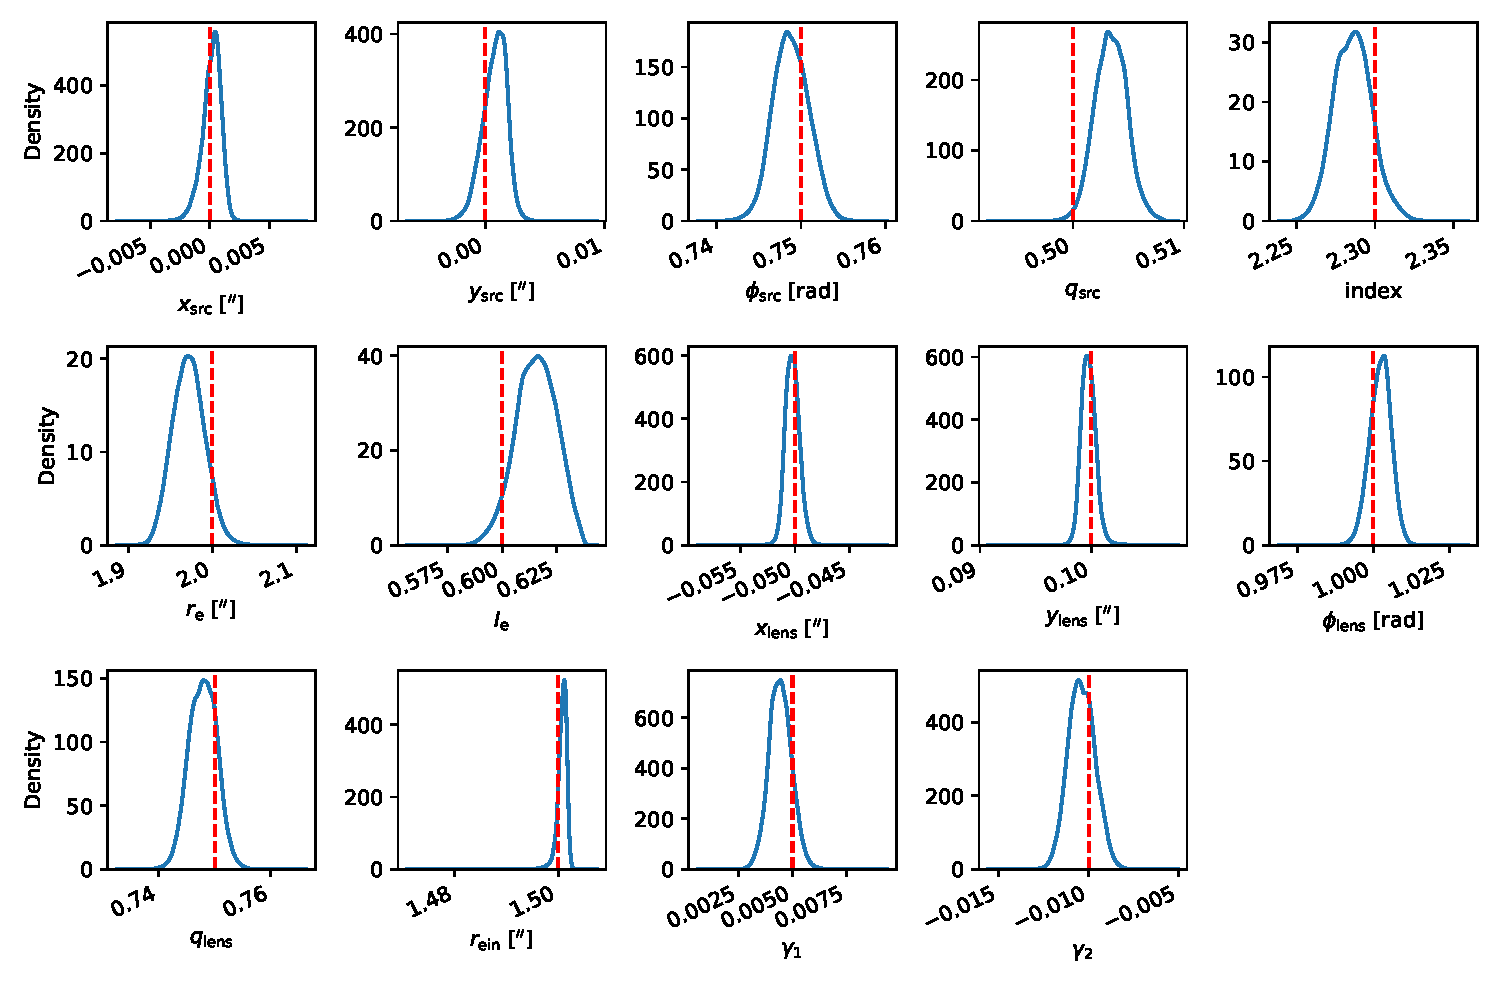
\includegraphics[width=0.9\linewidth]{GL-lss-macro-post.pdf}
    \caption{The 1D marginal posteriors for all macromodel parameters of the lensing system shown in Figure~\ref{fig:gl-lss-sub-post}. The posteriors were computed using a \gls*{cnn}-based ratio estimator. The first seven panels correspond to the source parameters, the next five are for the main lens and the last two are for the external shear. All posteriors encompass the true parameter values (vertical red dashed lines) within the $\sim 2\sigma$ interval.}
    \label{fig:gl-lss-macro-post}
\end{figure*}

\begin{figure*}
    \centering
    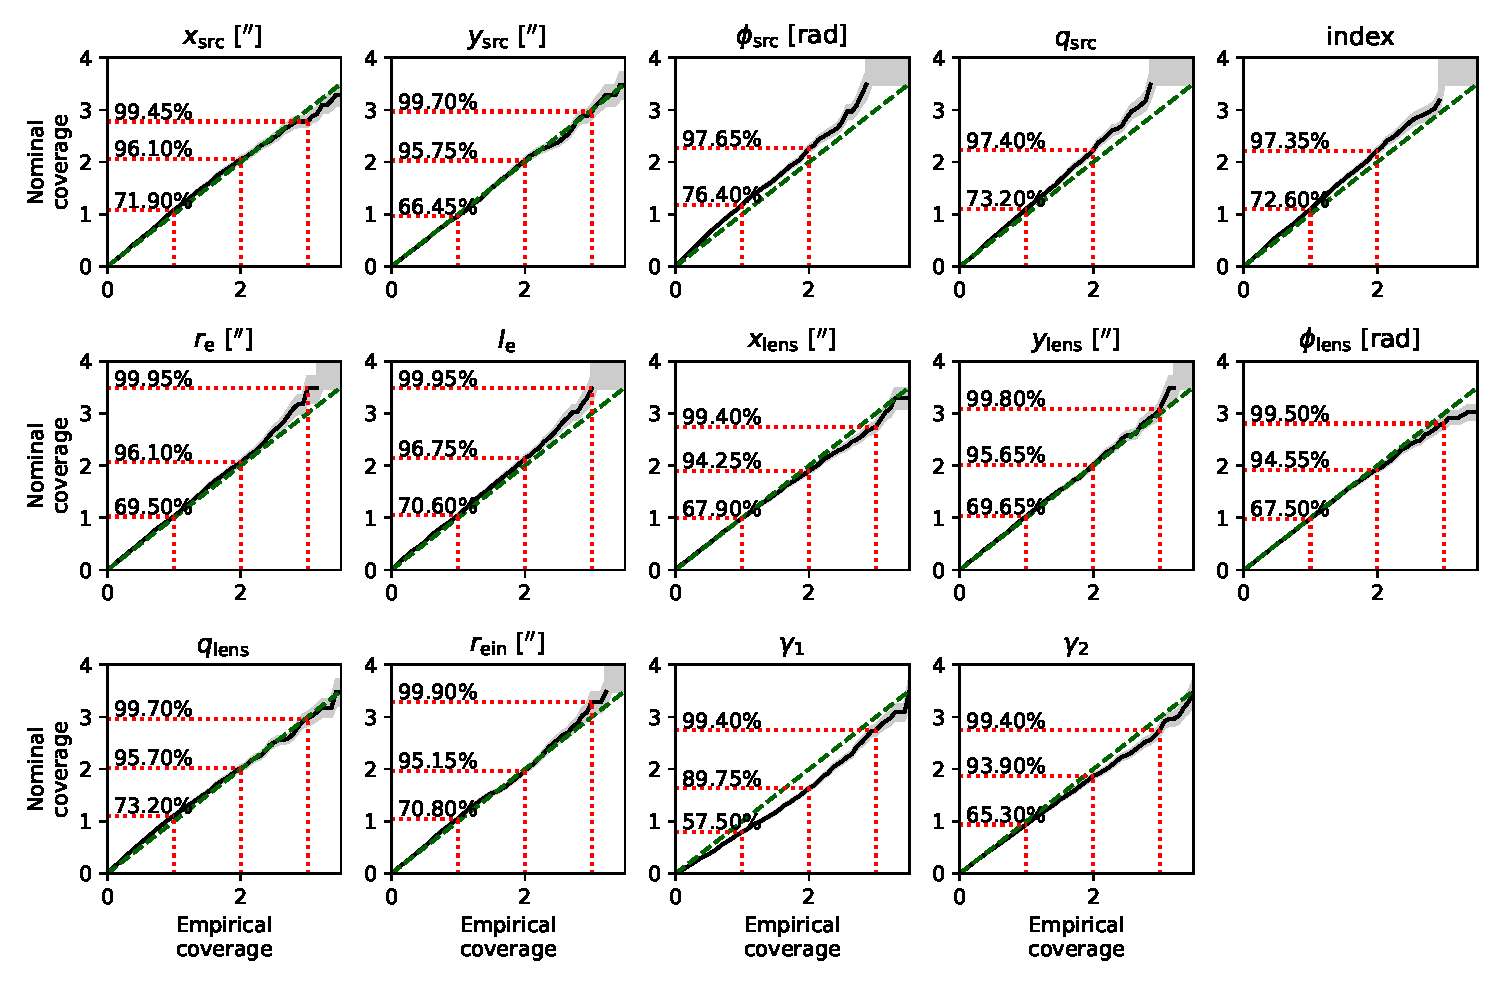
\includegraphics[width=0.84\linewidth]{GL-lss-macro-coverage.pdf}
    \caption{Coverage plots for the 1D marginal macromodel parameter posteriors of the lensing system from Figure~\ref{fig:gl-lss-sub-post}, using the same format as in Figure~\ref{fig:gl-sp-coverage}. The posteriors generally have coverage, with a few being slightly conservative ($\phi_s$, $q_s$ and the source index) and the shear posteriors being slightly overconfident.}
    \label{fig:gl-lss-macro-coverage}
\end{figure*}

\subsection{Subhalo mass and position inference with a population of perturbers}
\label{sec:lshs}

For our final inference task we extend the previous one by aiming to infer the position and mass of a relatively heavy target subhalo while marginalizing over a population of lighter perturbers of unknown size. The priors for the perturber population are summarized in Table~\ref{tab:params-and-priors} and Section~\ref{subsec:substructure}. Our lensing images contain on average about \num{260} \gls*{los} halos and \num{3} subhalos in the lens plane. This means on average about \num{800} parameters are required to describe such images. Likelihood-based sampling of this high-dimensional, transdimensional posterior requires techniques such as reversible-jump \gls*{mcmc} \citep{Daylan:2017kfh,Brewer:2015yya}. To marginalize over the perturber population with \gls*{tmnre}, their parameters are sampled over during data generation but not passed to the ratio estimator.

Since the population of perturbers can contain a member with mass greater than our target subhalo, we need to make this inference task well-defined by ``labeling'' the subhalos of interest. We accomplish this by making the perturber population lighter than the target subhalo, with mass restricted to the range $10^7-10^8\si{\solmass}$. We further assume the target subhalo has been localized to a $\SI{1.4}{''}\times\SI{1.4}{''}$ patch of the image around its true position.

The final-round inference results for $\psubb$ plotted in Figure~\ref{fig:gl-lshs-post} show that inclusion of the perturber population has a substantial effect on the posteriors. The posterior for the subhalo's mass peaks around the true value, but has a long tail extending towards the lower boundary of the prior. This indicates we are only able to obtain an upper bound on the subhalo mass rather than a measurement, and cannot exclude the possibility its mass is the lowest value consistent with the prior. Having validated our analysis in simpler cases and checked our ratio estimator has good coverage, we conclude our marginal posteriors are in fact close to the true ones.

%This is consistent with the fact the target subhalo's prior region contains on average \num{20} subhalos with total mass around \SI{1.5e9}{\solarmass}.
Our results are roughly in line with the image segmentation analysis of \cite{Ostdiek:2020cqz,Ostdiek:2020mvo}, which found subhalos of mass above roughly  $10^{8.5}\si{\solmass}$ were resolvable in similar mock observations. In addition, while the 68\% credible region for the subhalo's position contains its true position, the 95\% and 99.7\% credible regions cover nearly the whole prior region.

The posteriors for the source and lens parameters are shown in Figure~\ref{fig:gl-lshs-macro-post}. While some of the parameters' posteriors have comparable widths to those found in the previous inference task (namely $\phi_{s/l}$, $q_{s/l}$, the source index, $I_e$, $\gamma_1$ and $\gamma_2$), others are measured much less precisely due to the stochastic perturber population ($x_{s/l}$, $y_{s/l}$, $r_e$ and $\theta_E$). We omit coverage plots for this analysis as they are of comparably-good quality to those in the previous subsection.

\begin{figure*}
    \centering
    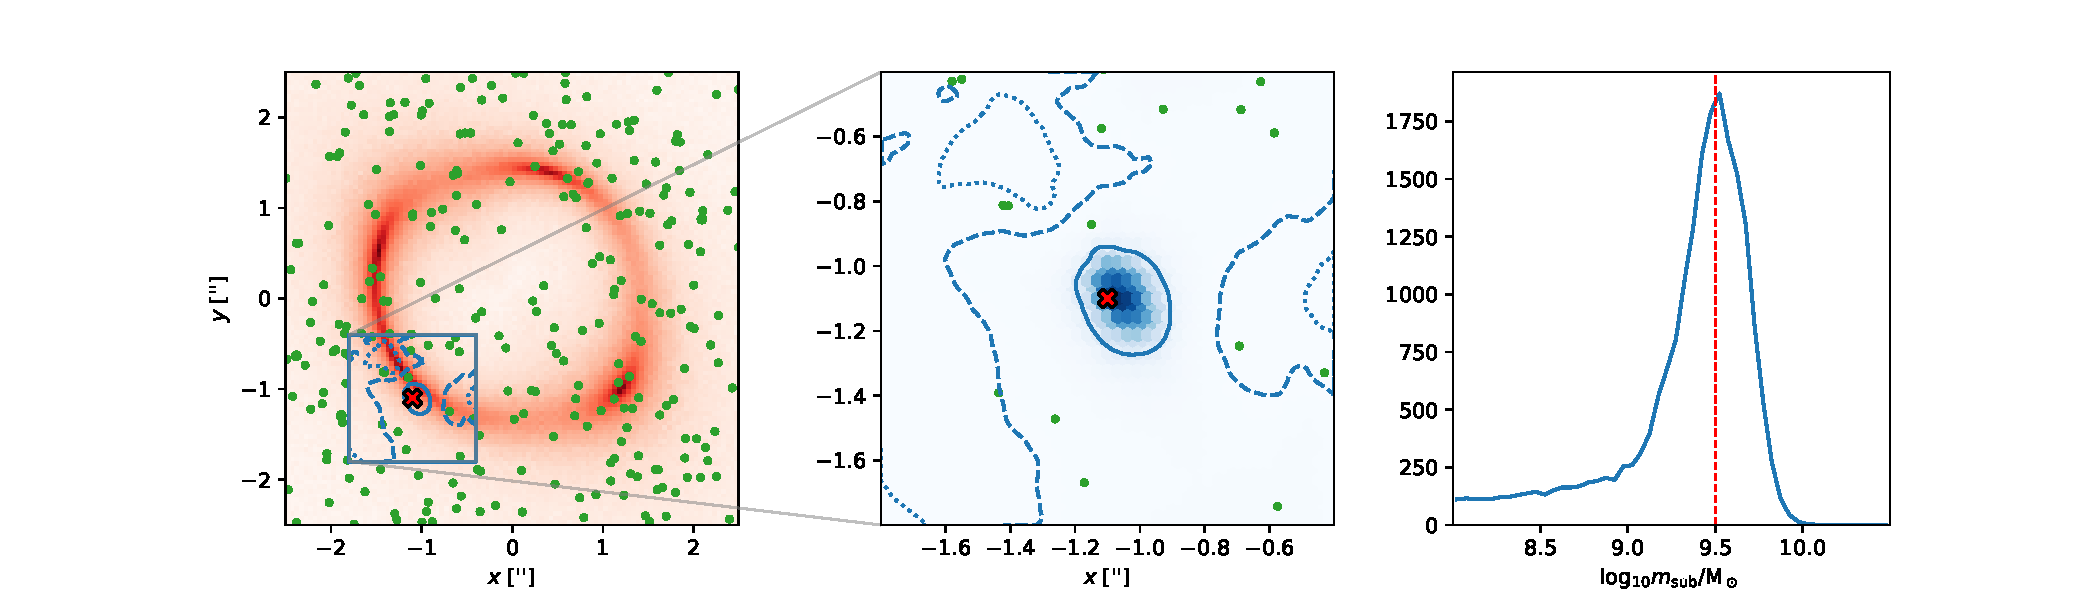
\includegraphics[width=\linewidth]{GL-lshs-post-2d.pdf}
    \caption{Subhalo position and mass posteriors obtained with \gls*{tmnre}, now marginalizing over a population of $10^7-10^8\si{\solmass}$ \gls*{los}/subhalos (green dots) in addition to the unknown macromodel. See the caption of Figure~\ref{fig:gl-lss-sub-post} for details. The initial prior for the subhalo's position is indicated by the blue box in the left panel. The range of the $x$-axis in the right panel shows the prior on the $\log_{10}$ of its mass. For both the subhalo's mass and position, the width of the inferred posteriors prevents \gls*{tmnre} from truncating the priors.}
    \label{fig:gl-lshs-post}
\end{figure*}

\begin{figure*}
    \centering
    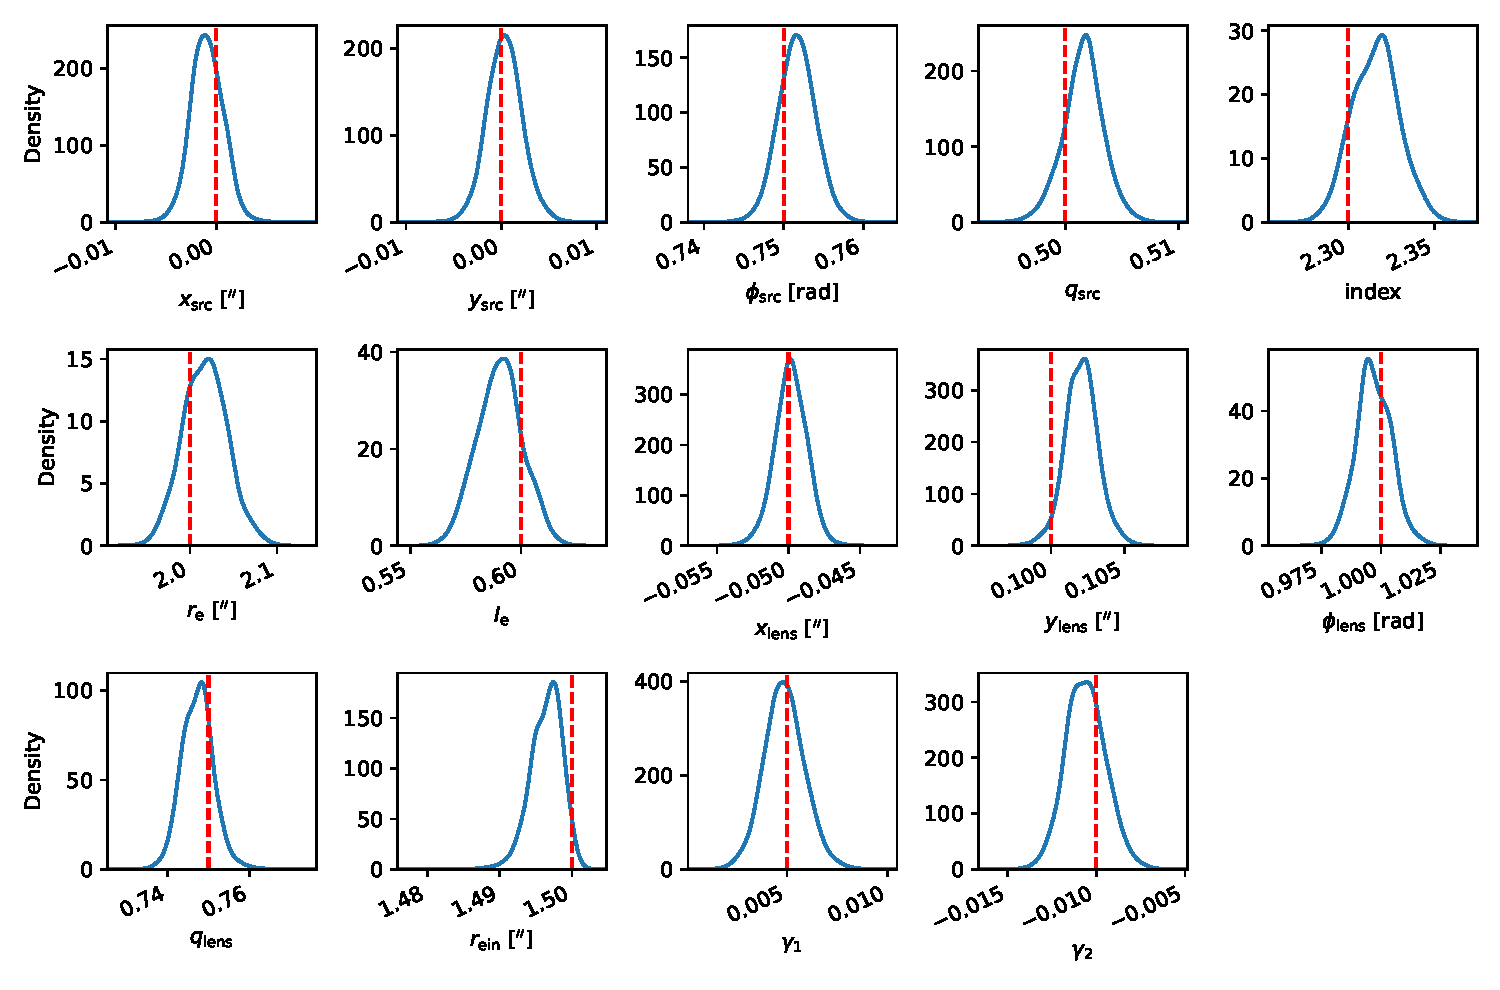
\includegraphics[width=0.84\linewidth]{GL-lshs-macro-post.pdf}
    \caption{Macromodel 1D marginal posteriors as in Figure~\ref{fig:gl-lss-macro-coverage}, but for the inference task where a population of $10^7-10^8\si{\solmass}$ are present in the observation. This has the effect of broadening most of the posteriors.}
    \label{fig:gl-lshs-macro-post}
\end{figure*}


\section{Hierarchical inference of dark matter mass} \label{sec:results-pop}

%A population of low-mass halos can collectively cause perturbations to images that can be detected statistically in order to constrain the \gls*{hmf}. 
%In reality, constraining collective substructure properties from gravitational lensing images is an extremely difficult problem. 
%From measuring the distributions of perturbers' masses and other parameters, it is possible to infer population-level properties like the (sub)halo mass function parameters, which are dictated by the fundamental properties of dark matter.

In this section, we show our results for hierarchical population parameters inference. First, we describe the simulated data in Section~\ref{subsec:pop-data} and the inference strategy in Section~\ref{subsec:pop-nn}. We then show how we constrain the lens and source parameters in Section~\ref{subsec:constrain}. Next, we show our results for the \gls*{hmf} cutoff mass and describe how we can combine the information from different strong lensing images in Section~\ref{subsec:dm}. In the same subsection, we show our results on the \gls*{dm} mass. Finally, we directly assess the statistical behaviour of the trained neural networks in Section~\ref{subsec:test}.

\subsection{Mock data generation}
\label{subsec:pop-data}

\begin{figure}
    \centering
    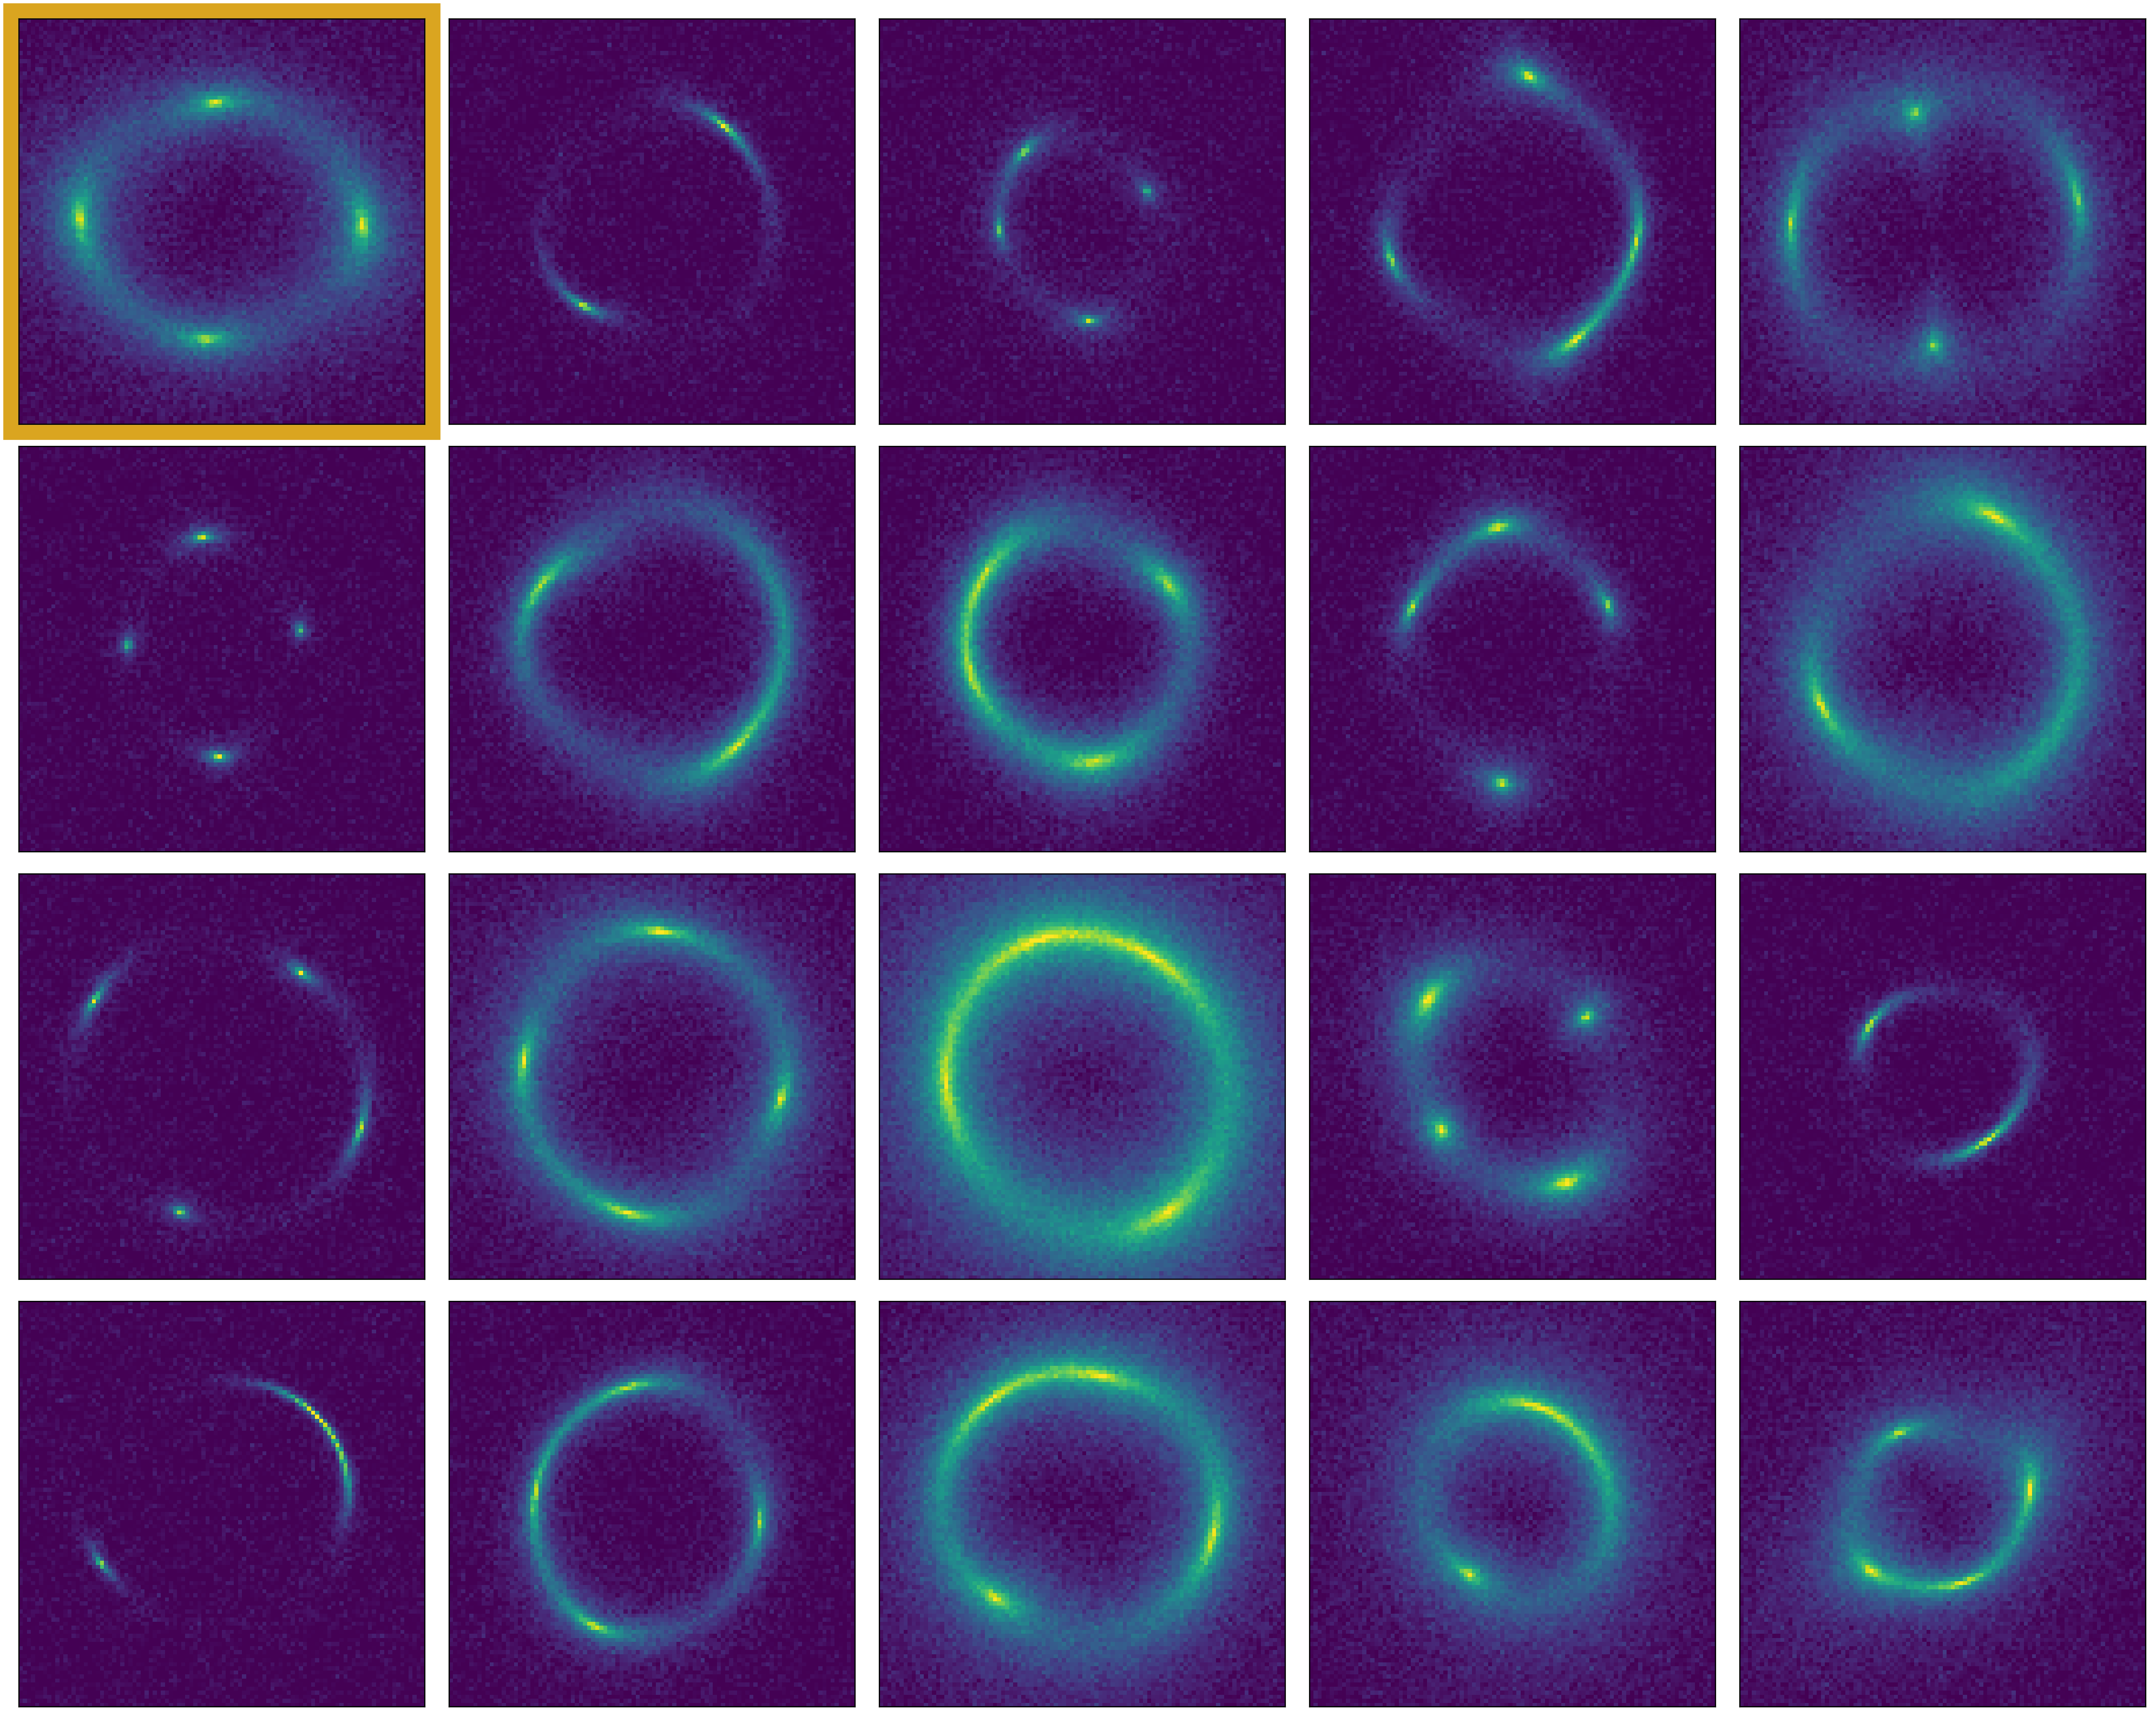
\includegraphics[width=\linewidth]{GL-mock.png}
    \caption{We present a gallery of twenty mock strong-lensing images we use as target observations. These mock observations have been generated with arbitrary lens and source parameters drawn from the initial prior in Table~\ref{tab:model}. Their peak \gls*{snr} is $\num{\sim 30}$, representative of \gls*{hst} data. We analyse these images by first constraining their lens and source parameters proposal distribution in Section~\ref{subsec:constrain}. Then, we combine them in order to infer the cutoff mass scale in Section~\ref{subsec:dm}. For the first one (upper left corner, framed in orange) of these images we show our results of the first part of the pipeline (Section~\ref{subsec:constrain}) in Figure~\ref{fig:bounds}, Figure~\ref{fig:targeted_data}, and Figure~\ref{fig:lens_source_post}.
}
\label{fig:mock}
\end{figure}

For this inference task we use our lensing simulator at its full capacity, by including lens, source, substructures and different \gls*{dm} models that depend on the half-mode-mass \mhm:
\begin{equation}
    p(\data\mid\psrc, \plens,\pp, \vartheta)
    = \mathcal{N}(\data\mid\mathrm{obs}(\psrc, \plens, \pp, \mhm), \sigma^2).
\end{equation}

In Figure~\ref{fig:mock} we show a gallery of twenty mock strong-lensing images we use as target observations. These mock observations have been generated with arbitrary lens and source parameters drawn from the initial prior in Table~\ref{tab:pop-model}.


\begin{table}
\begin{center}
\resizebox{0.9\columnwidth}{!}{%
    \begin{tabular}{l l l c }
        \toprule
        Parameter & {True value} & Prior & Description \\
        \midrule
        \textbf{Main lens} &  &  &  SPLE \\
        $\theta_E$ [\si{\arcsecond}] &  & $\Uniform(1.,2.)$  & Einstein radius \\
        $\xi_{0,x}$ [\si{\arcsecond}] &  & $\Uniform(-0.2,0.2)$  & lens center x axis \\
        $\xi_{0,y}$ [\si{\arcsecond}] &  & $\Uniform(-0.2,0.2)$  & lens center y axis \\
        $q_l$ &  & $\Uniform(0.1,1.)$ & axis ratio \\
        $\phi_l$ [\si{\radian}]&  & $\Uniform(0,2\pi)$  & rotation angle \\
        $\gamma$ & 2.1 & -  & slope \\
        $z_\mathrm{lens}$ & 0.5 & -  & lens redshift \\
        \midrule
        \textbf{External shear}  &  &  &   \\
        $\gamma_1$ &  & $\Uniform(-0.05,0.05)$  & $1^{\mathrm{st}}$ component\\
        $\gamma_2$ &  & $\Uniform(-0.05,0.05)$   & $2^{\mathrm{nd}}$ component\\
        \midrule
        \textbf{Source} &  &  &  Sérsic \\
        $I_e$ &  & $\Uniform(0.,4.)$  & surface intensity \\
        $r_e$ [\si{\arcsecond}] &  &  $\Uniform(0.1,2.5)$ & effective radius \\
        $x_0$ [\si{\arcsecond}] &  & $\Uniform(-0.1,0.1)$ & source center x axis\\
        $y_0$ [\si{\arcsecond}] &  & $\Uniform(-0.1,0.1)$ & source center y axis\\
        $q_s$ &  & $\Uniform(0.1,1.)$ & axis ratio\\
        $\phi_s$ [\si{\radian}] &  &  $\Uniform(0,2\pi)$  & position angle\\
        $n$&  &  $\Uniform(0.1,4.)$  & index\\
        $z_\mathrm{src}$ & 2 & -  & source redshift\\
        \midrule
        \textbf{Subhalos} & & &  tNFW \\
        $\vec{p}$ [\si{\arcsecond}] & {$\in[-2.5, 2.5]$} & $\Uniform_{2\mathrm{D}}(-2.5, 2.5)$ & position\\
        $m_{200}$ [\si{\solmass}] & {$\in[10^7, 10^{10}]$} & \cite{Giocoli:2009ie} & virial mass\\
        $c_{200}$ & 15. & - & concentration \\
        $\tau$ & 6. & - & truncation\\
        \midrule
        \textbf{\gls*{los} halos} &  &  &  projected tNFW \\
        $\vec{p}$ [\si{\arcsecond}] & {$\in[-2.5, 2.5]$} & $\Uniform_{2\mathrm{D}}(-2.5, 2.5)$ & position\\
        $m_{200}$ [\si{\solmass}] & {$\in[10^7, 10^{10}]$} & \cite{Tinker:2008ff} & virial mass\\
        $z_{\mathrm{LOS}}$ & {$\in[0, z_\mathrm{src}]$} &  \cite{Tinker:2008ff} & LOS redshift\\
        $c_{200}$ & 15. & - & concentration \\
        $\tau$ & 6. & - & truncation\\
        \midrule
        \textbf{\gls*{wdm}} &  & &  \\
        $\mhm$ [\si{\solmass}] & & $\log\Uniform(10^7, 10^{10})$ & half-mode mass\\
        \bottomrule
    \end{tabular}
}
\end{center}
\caption{Summary of model parameters used for the simulated images in this work. When a prior distribution is not specified, the parameter is fixed to the true value.}
\label{tab:pop-model}
\end{table}


\subsection{Inference strategy}
\label{subsec:pop-nn}

The inference neural network used to perform \gls*{tmnre} is split into two different components: an embedding network $C_\phi(\data)$ and a binary classification network. 
The embedding network compresses data into a low-dimensional feature vector, estimating the best possible summary statistics from the full input image. 
The binary classification network is the marginal classifier that performs the actual ratio estimation. It passes the featurized observational data concatenated with the parameter of interest into a \gls*{mlp} to estimate the marginal likelihood-to-evidence ratios.
The network architecture can be expressed as:
\begin{equation}
    d_\phi(\data, \vartheta) = \mathrm{MLP}_\phi(\text{features} = C_\phi(\data), \vartheta) = \sigma[ \log \hat{r}(\data, \vartheta)].
\end{equation}

For the embedding network, in both steps of the pipeline, we adopt a simple \gls*{cnn}. In Figure~\ref{fig:cnn} we show the \gls*{cnn} architecture used to constrain lens and source parameters. The one used to estimate the cutoff mass has a similar structure.

\begin{figure}
\centering
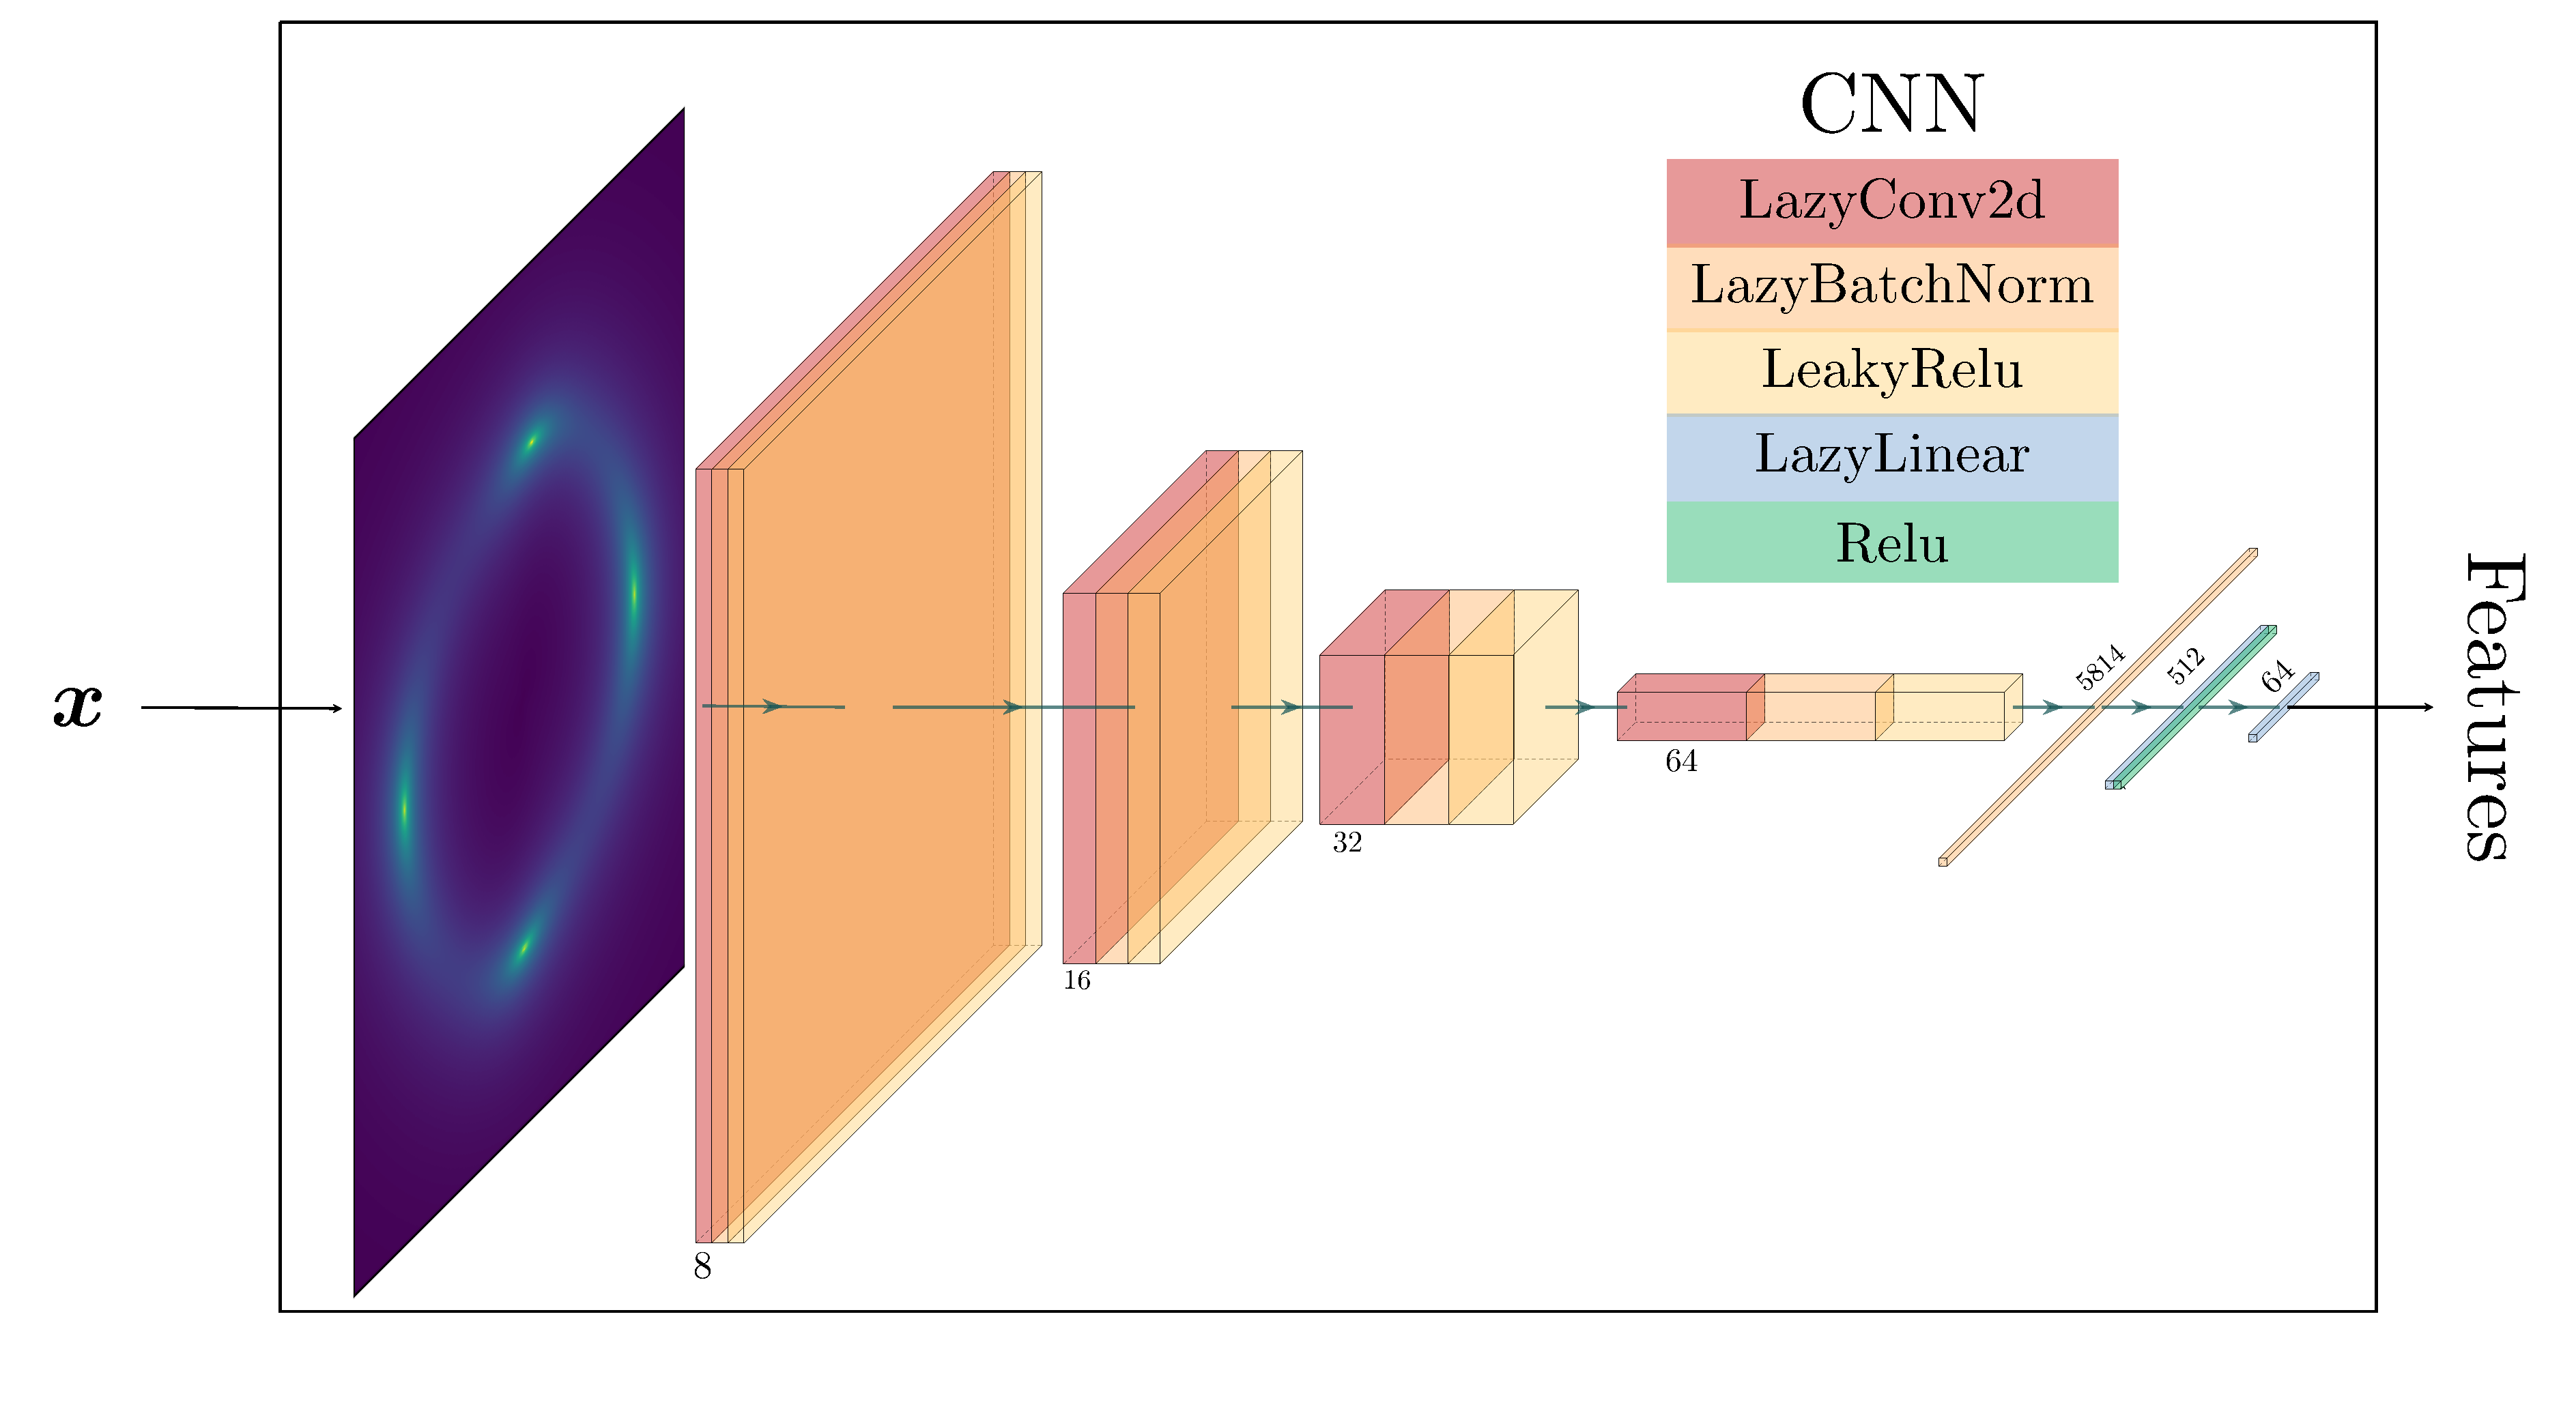
\includegraphics[width=\linewidth]{GL-cnn.pdf}
\caption{Illustration of the embedding \gls*{cnn} architecture used in the first part of the pipeline to constrain lens and source parameters. The observation $\data$ gets compressed into features: estimates of the best possible data summary statistic, by the \gls*{cnn}. In describing the \gls*{cnn} layers we follow \texttt{PyTorch} \citep{pytorch} convention. To create the illustration we have used \cite{PlotNeuralNet}.
}
\label{fig:cnn}
\end{figure}


\subsection{Constraining lens and source parameters}\label{subsec:constrain}

\begin{figure*}
\centering
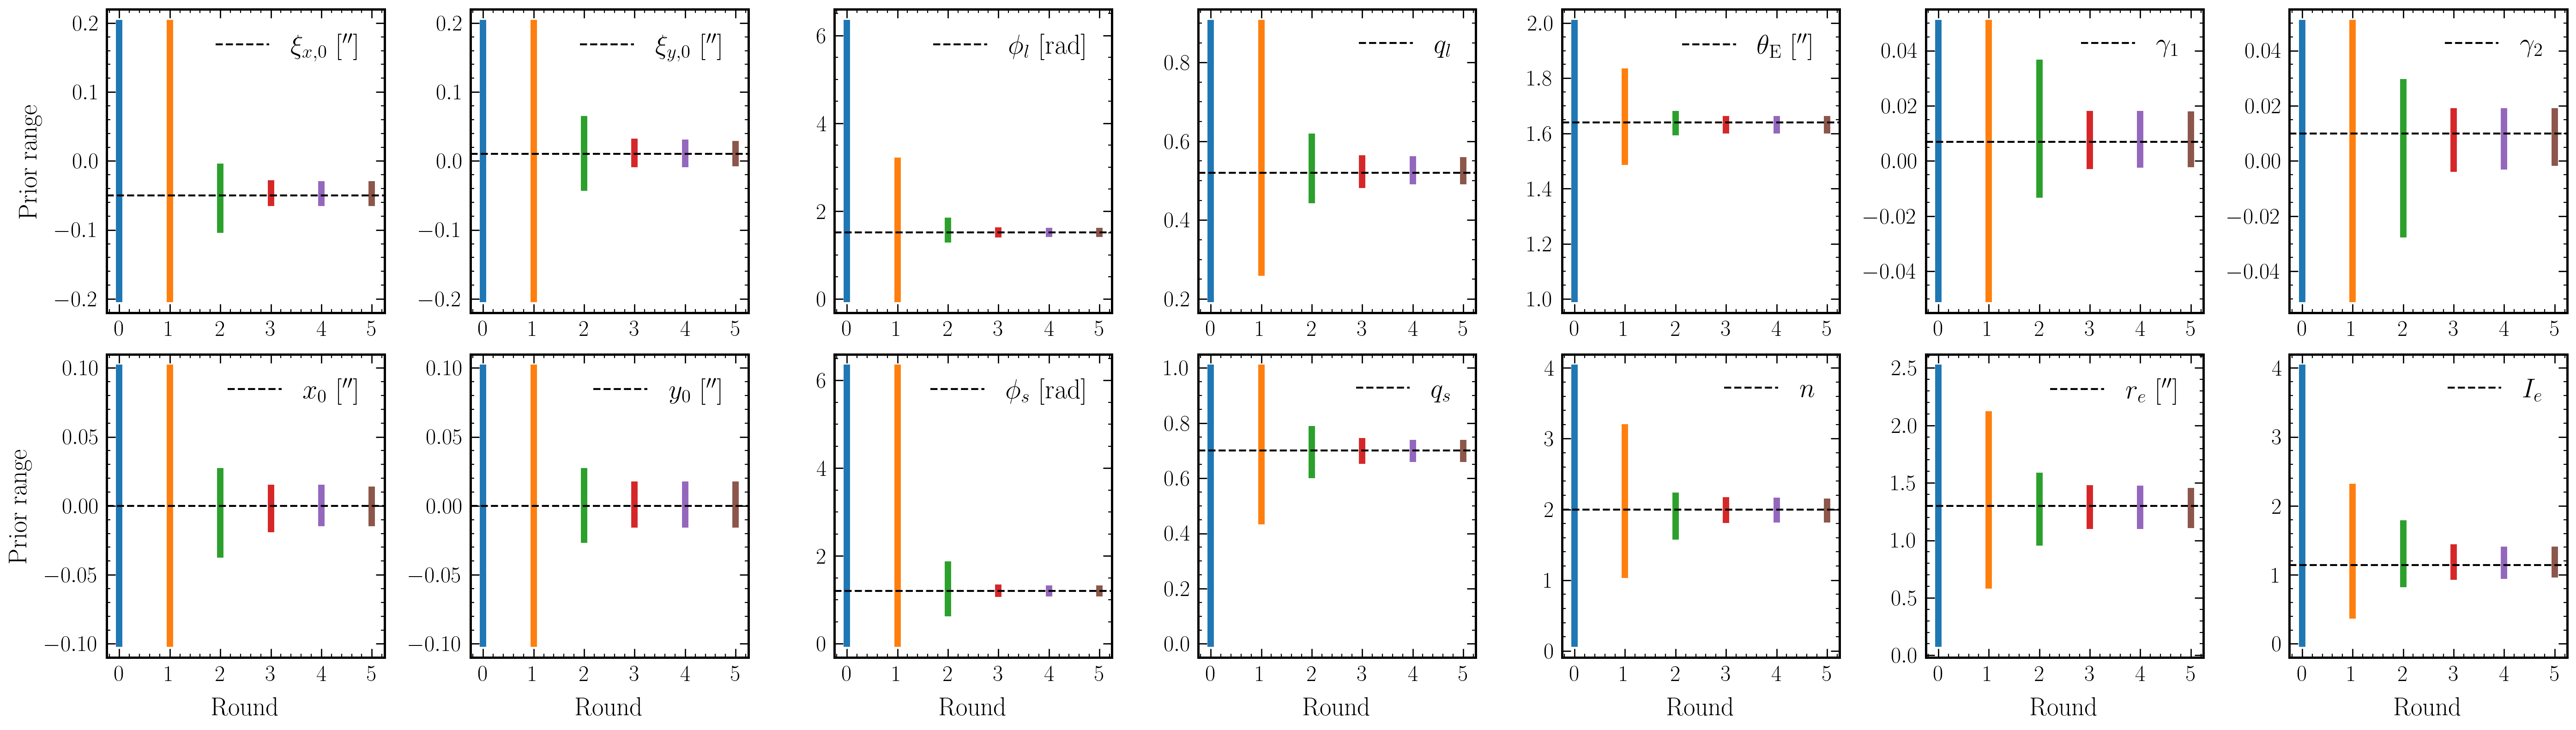
\includegraphics[width=\linewidth]{GL-bounds.png}
\caption{Constrained proposal distribution. Visualization of the sequential truncation of the lens and source proposal distributions over the six rounds of training. The particular target is the first mock image (framed in orange in Figure~\ref{fig:mock}), whose parameters are depicted as black dashed horizontal lines.
}
\label{fig:bounds}
\end{figure*}

\begin{figure}
\centering
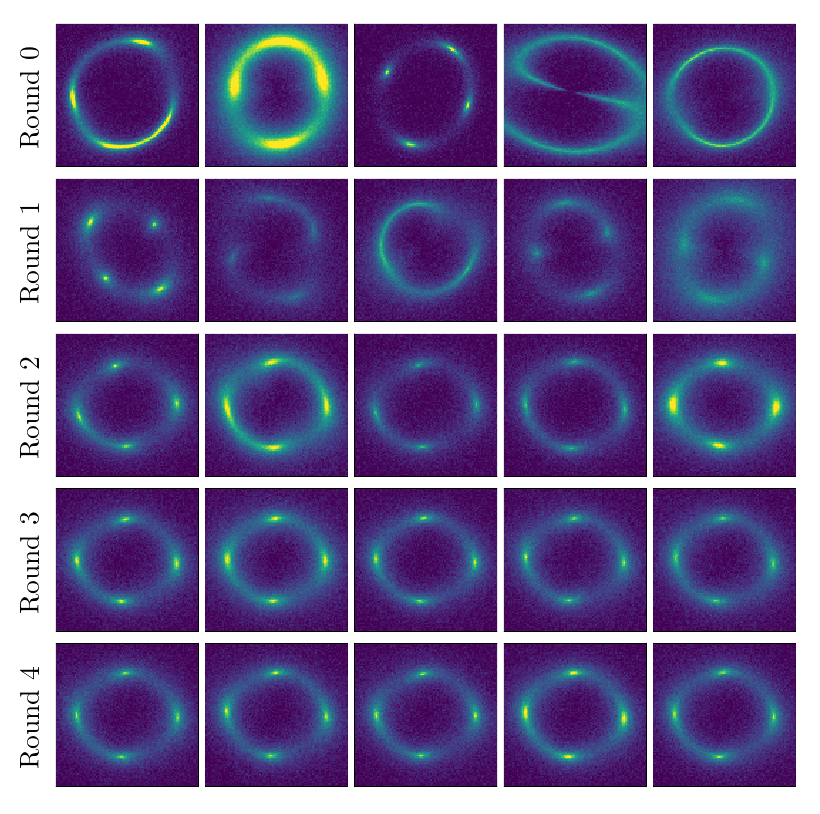
\includegraphics[width=\linewidth]{GL-targeted_data.png}
\caption{Training data targeting the first mock observation (framed in orange in Figure~\ref{fig:mock}). In each row, we show five examples of training data for the first five rounds. In the first round, we sample our data from the initial prior shown in Table~\ref{tab:pop-model}. For the following rounds, the lens and source parameters are sampled from the constrained proposal distributions, obtained by evaluating the network trained with the previous round dataset on our target observation (see Section~\ref{subsec:constrain}). It is evident that with each round the training data more closely resembles the target image $\data_0$.
}
\label{fig:targeted_data}
\end{figure}

\begin{figure*}
\centering
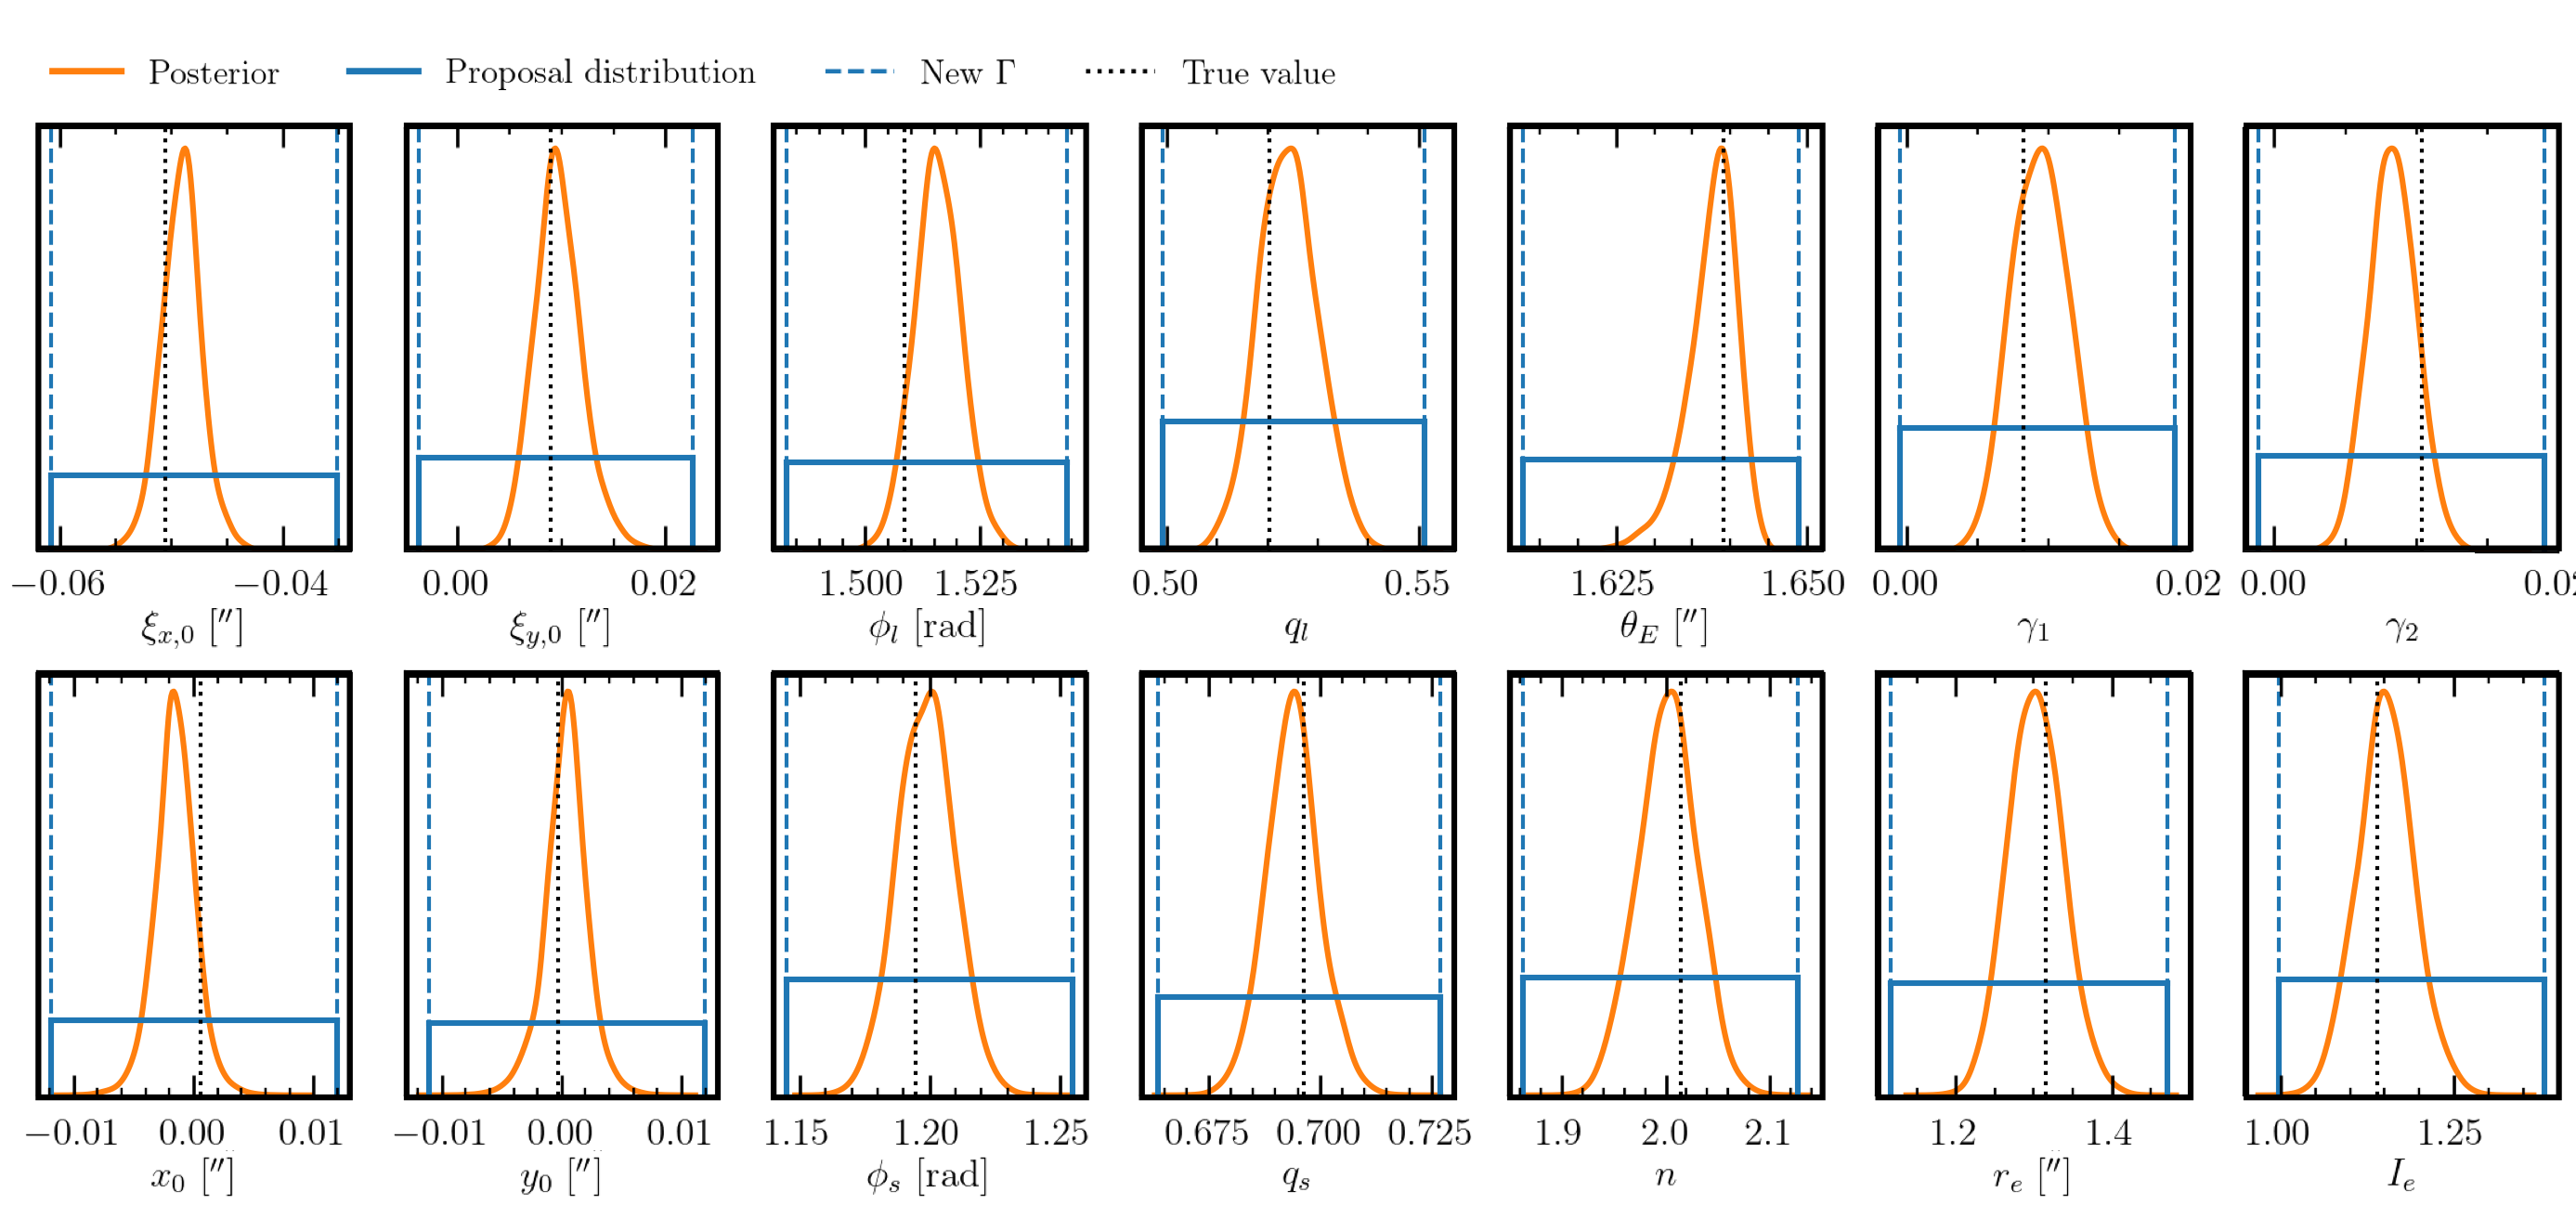
\includegraphics[width=\linewidth]{GL-lens_source_post.png}
\caption{Lens and source parameters posteriors. In solid blue we show the last round of constrained proposal distributions for the first (upper left corner, framed in orange) target image in Figure~\ref{fig:mock}. The dotted black lines correspond to the true lens and source parameters values with which we have generated the target image. In orange, we show the estimated posteriors for lens and source parameters in the last training round. Based on the predetermined threshold, the new bounding limits $\Gamma$ (dashed blue) do not change significantly from the previous constrained proposal distribution region, so it is not possible to constrain the proposal distribution more and we stop the truncation procedure.
}
\label{fig:lens_source_post}
\end{figure*}

We constrain lens and source parameters regions with \gls*{tmnre} (Section~\ref{sec:sbi-tmnre}) with multiple sampling and training rounds.

In total, we perform six sampling and training rounds. In each round, we simulate $10^5$ observations, of which $90\%$ are used as the training dataset, and the remaining $10\%$ as the validation dataset. Evaluations of the network on the mock target image are used to truncate the  training data proposal distribution after each round, so that the region for lens and source parameters is targeted. The first training round is performed on the dataset generated from the initial source and lens parameters priors, shown in Table~\ref{tab:pop-model}. In Figure~\ref{fig:bounds} we show the initial prior and the following constrained proposal distributions. It can be seen that after the first round just a few of the parameters proposal distributions get truncated, \eg~the Einstein radius. By having truncated these initial parameters, in the following rounds the other parameters can be better learned by the network and so constrained. In Figure~\ref{fig:targeted_data}, we show samples from the first five training datasets, which demonstrate that the constrained regions are indeed the ones that are likely to produce data similar to the targeted image $\data$. After the sixth round of training, it is not possible anymore to truncate the proposal distribution region based on the predetermined threshold, as seen in Figure~\ref{fig:lens_source_post}. The truncation scheme has then efficiently identified the constrained region for lens and source parameters consistent with the targeted observation. Using the last constrained dataset, it is then easier in the second step of the pipeline to train a marginal neural ratio estimator to perform the final inference on the cutoff mass.

We would like to stress that these constrained proposal distributions correctly account for lens and source parameters uncertainties. In all our simulated data, the substructure parameters $\pp$ are randomly sampled from their prior, in order to account for the presence of substructure. This has the desirable outcome of approximately accounting for the average effect that an additional mass component has on the main lens parameters (\eg\ inferring an unbiased Einstein radius) and contributes to the source and lens uncertainties.

\subsection{Dark matter inference}
\label{subsec:dm}
For the second step of the pipeline, we train an inference network to learn the cutoff mass on the last constrained dataset. 

From initial tests, we have found that features from a single image are very hard to learn for the classifier, resulting in a very noisy ratio estimator.
In order to reduce the estimator uncertainty, we then train the cutoff mass classifier on a dataset $X^N=\{\data_1, ..., \data_N\}$ of $N$ different observations. For each observation, first, we constrain its lens and source parameters as explained in Section~\ref{subsec:constrain}. Then, we train the cutoff classifier on the concatenation of the features coming from their embedding networks, effectively learning $r(\mhm; X^N)$. 
Note that the images in one dataset are sampled with the same cutoff mass $\mhm$, but different lens, source, and substructures realizations. In fact, our final goal is to apply the full pipeline to real data, which will all have different source, lens, and substructures configurations, but will have encoded the same \gls*{dm} properties. 

\begin{figure*}
\centering
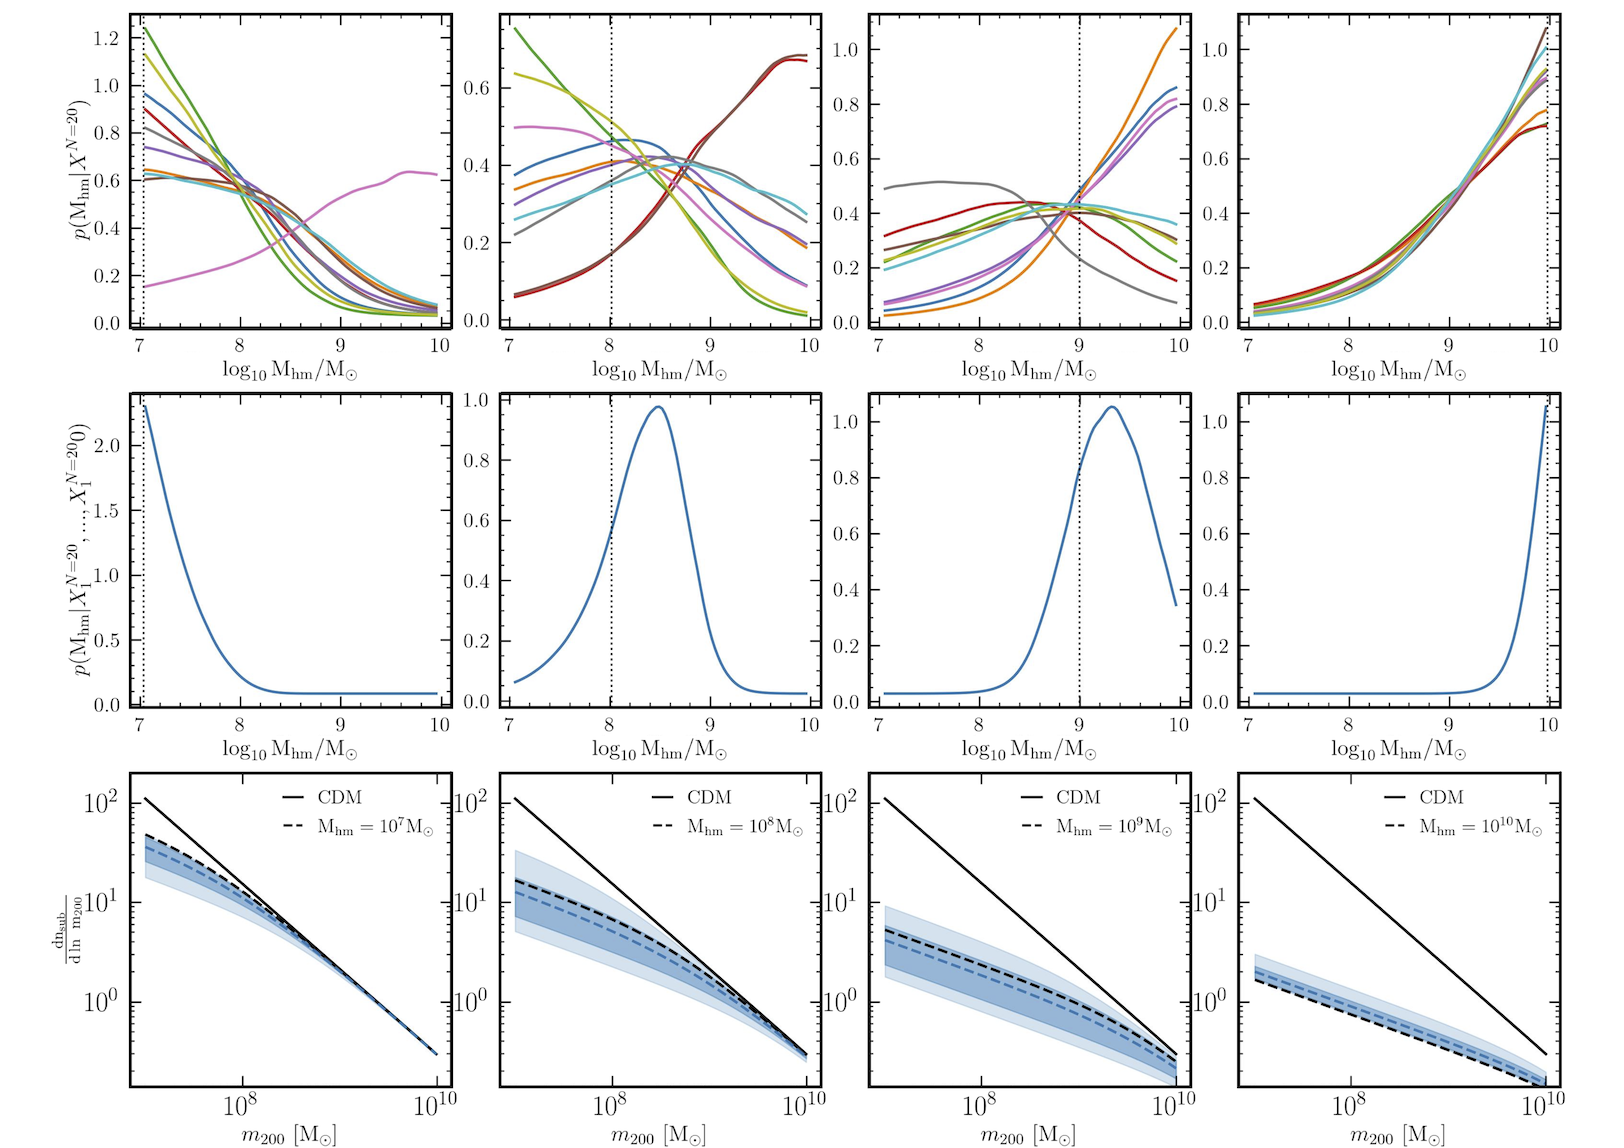
\includegraphics[width=\linewidth]{GL-mhm_results.png}
\caption{\textit{Top:} Approximate posteriors for the half-mode mass derived from 10 different sets of 20 images. The dotted black line represents the true value of the half mode mass with which we have generated the images ($10^7, 10^8, 10^9,  10^{10} \ \si{\solmass}$). 
\textit{Middle:} We show the approximate posterior resulting from the combination of the $M=10$ different posteriors shown in the first column, as explained in the text (Section~\ref{subsec:dm}).
\textit{Bottom:} Subhalo mass function constraints derived from the cutoff mass posterior shown in the second column. The black solid line shows the \gls*{cdm} subhalo mass function according to Equation~\eqref{eq:shmf}, whereas the black dashed one shows the \gls*{wdm} subhalo mass function according to Equation~\eqref{eq:cutoff}, given the true cutoff mass shown in the label. The blue dashed line shows the mean of the \gls*{wdm} subhalo mass function obtained by sampling $1000$ samples from the cutoff mass posterior shown in the second panel and using this value in Equation~\eqref{eq:cutoff}. We also show the central \num{68} and \num{95} percentiles as shaded bands. These plots show how uncertain the subhalo mass function is under the assumption that it has the functional form in Equation~\eqref{eq:cutoff} with parameters from \cite{Lovell:2020bcy}.
}
\label{fig:mhm_results}
\end{figure*}

In the first row of Figure~\ref{fig:mhm_results} we show the results from the inference network on ten test sets of lenses generated with a $\mhm$ value of $10^7, 10^8, 10^9$ and, $10^{10} \ \si{\solmass}$. Each curve is the posterior obtained for a set of $N=20$ lenses. Each of the mock observations has lens and source parameters sampled from their own final constrained proposal distribution, and different substructure population.  

Now that we have reduced the estimator noise, it is straightforward to perform inference on a group of sets of images by combining their ratios. Given a dataset $X^N=\{\data_1, ..., \data_N\}$ of images, the combined ratio for multiple $M$ datasets is simply given by $r(\mhm;X^N_M,) \propto \prod_{i=1}^M r(\mhm; X^N_i)$, where the proportionality is a ratio of evidences, independent of the parameter value, so it only accounts for a proper normalisation \citep{Brehmer:2019jyt, Hermans:2019ioj}.
In the second row of Figure~\ref{fig:mhm_results} we show the results for the combination of the $M=10$ different posteriors shown in the first column.

In the third row we show a combined posterior for the \gls*{wdm} mass function from 200 images ($M=10$ sets of $N=20$ images). These plots show the uncertainty in the subhalo mass function under the assumption that it has the functional form in Equation~\eqref{eq:cutoff} with parameters from \cite{Lovell:2020bcy}.

These first results show that our method is sensitive to the low-mass end of the \gls*{hmf}, and that we have unbiased results from combining just 10 sets of 20 observations, given that in the second panel of Figure~\ref{fig:mhm_results} the true input value for the half-mode mass $\mhm$ is consistently contained within the estimated posterior. In Section~\ref{subsec:test} we will show a more sophisticated method to assess the statistical behaviour of
our inference results.

\begin{figure*}
\centering
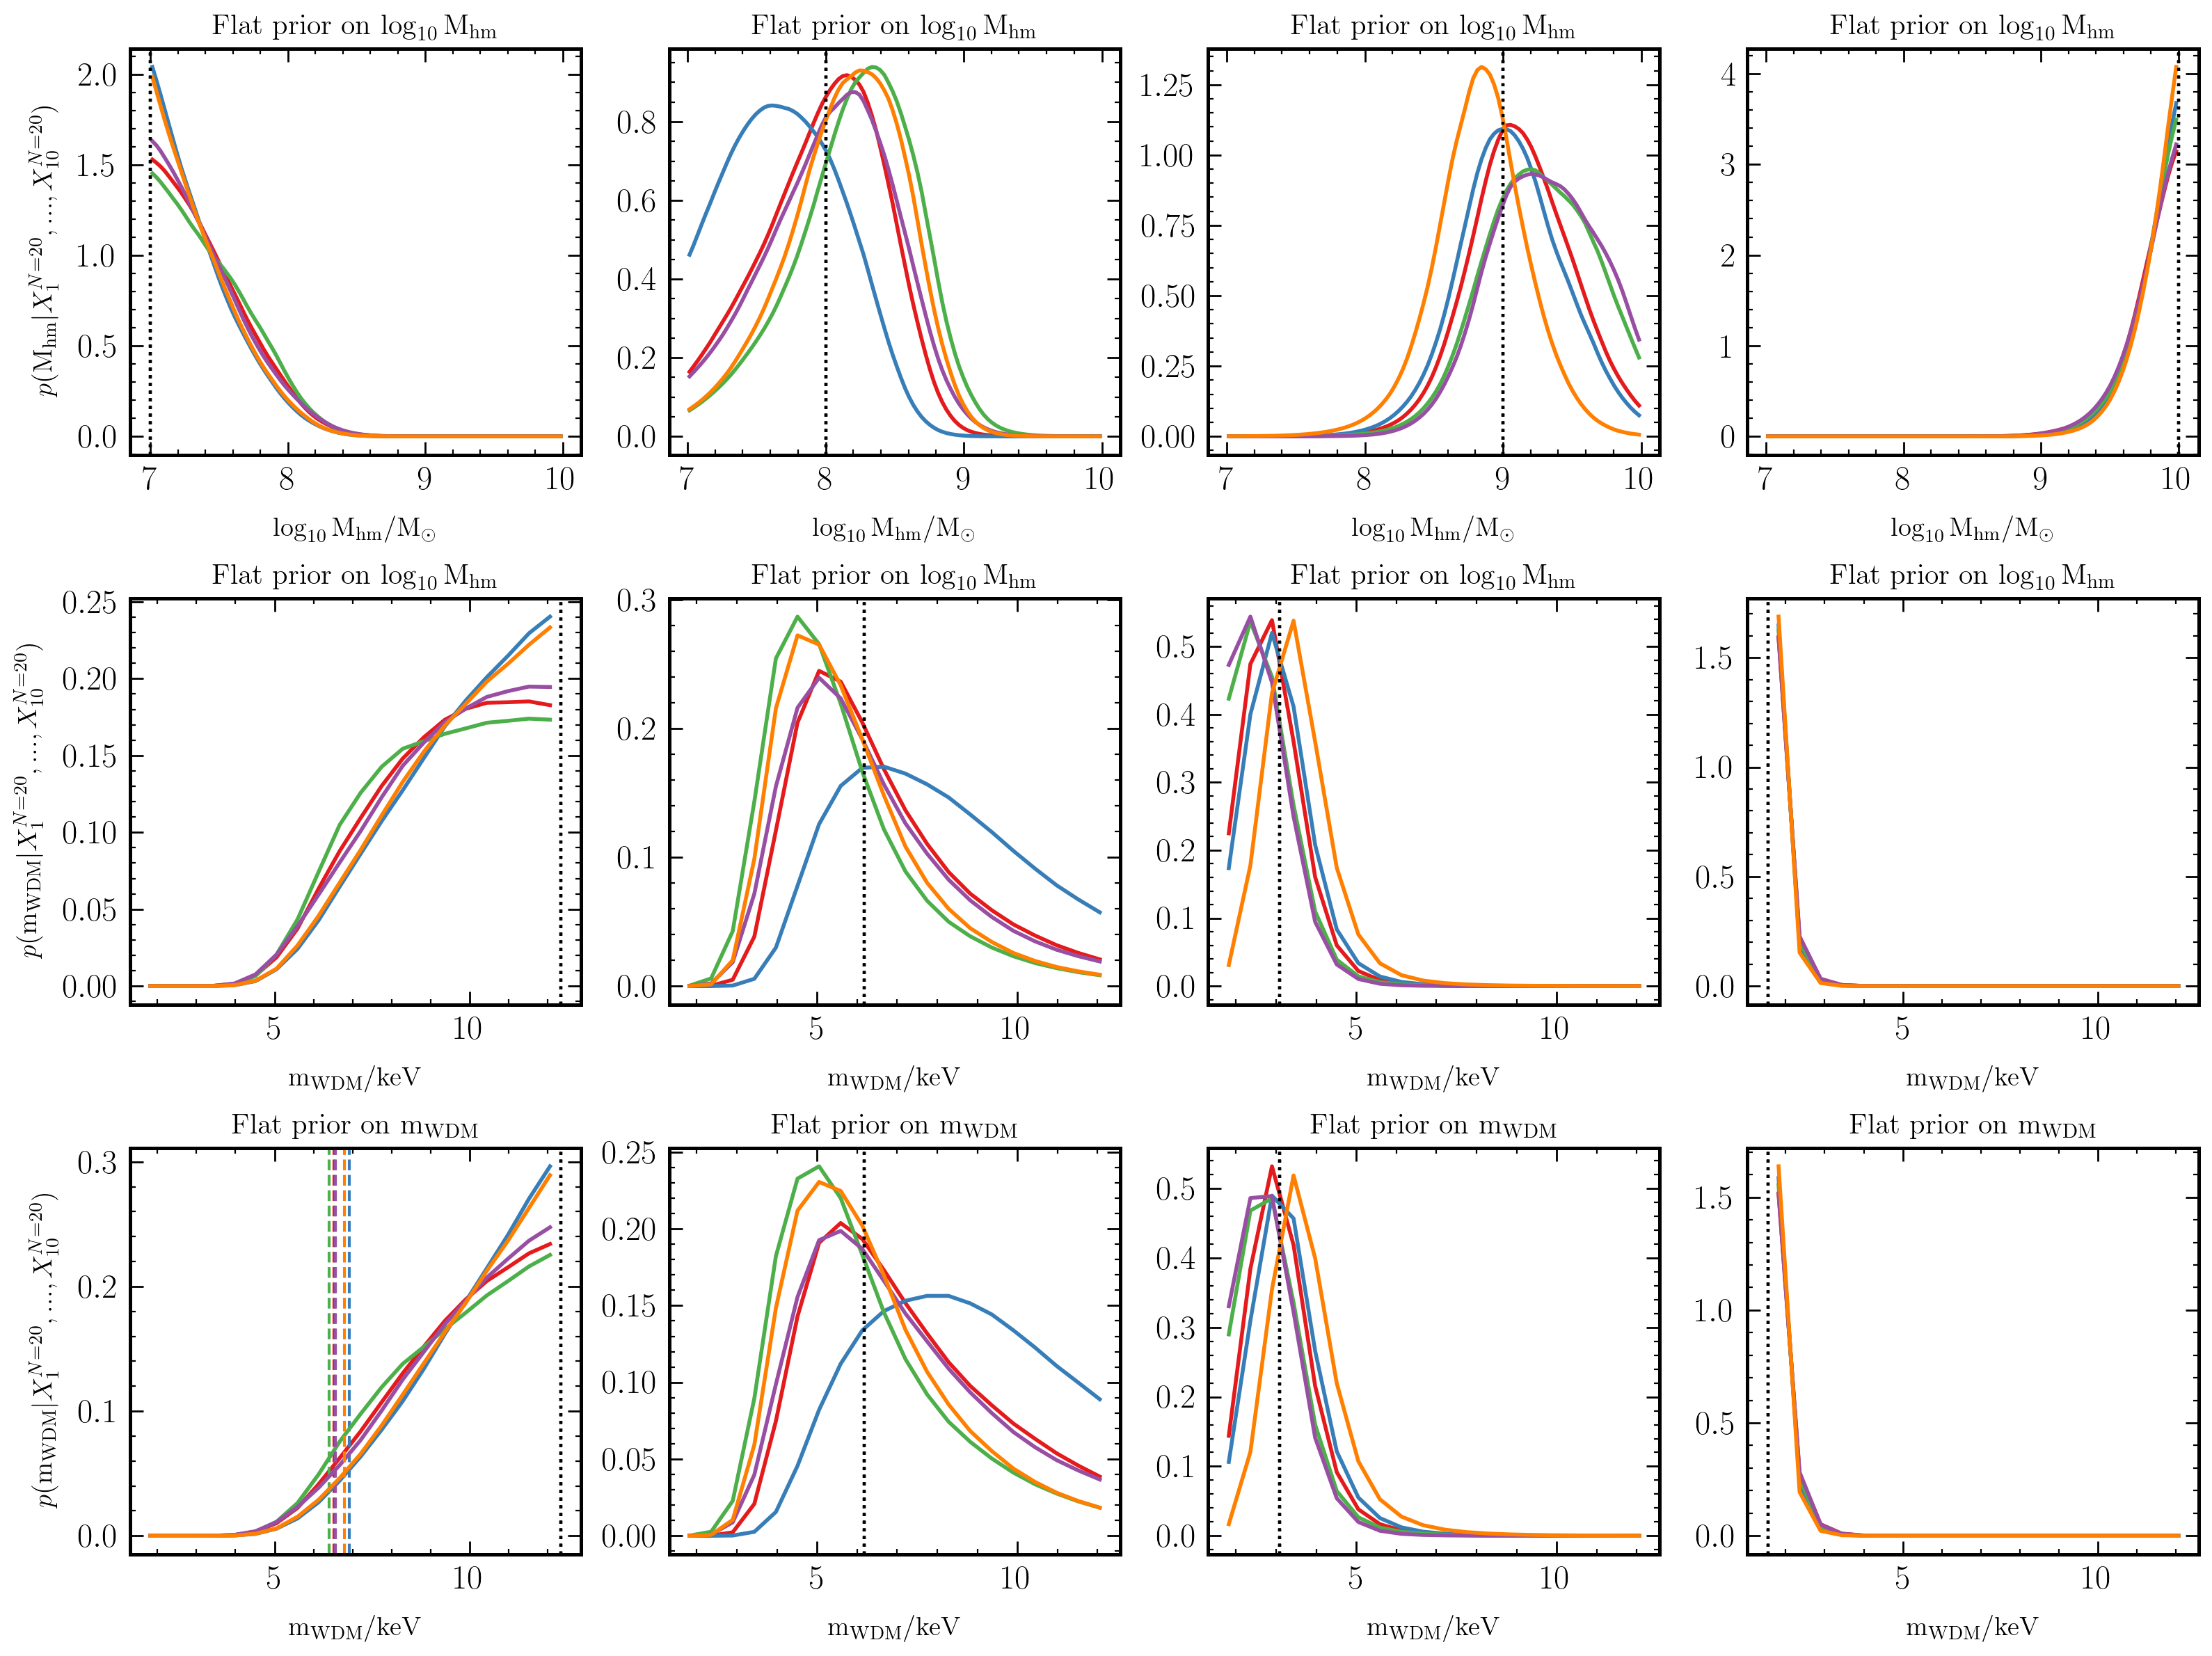
\includegraphics[width=\linewidth]{GL-wdm_results.png}
\caption{\textit{Top:} We show five examples of combined posterior of $M=10$ sets of $N=20$ observations in terms of the cutoff mass (as the second row in Figure~\ref{fig:mhm_results}). The dotted black line represents the true input value of the half mode mass with which we have generated the analyzed mock observations ($10^7, 10^8, 10^9,  10^{10} \ \si{\solmass}$). 
\textit{Middle:} Same results as shown in the first column but for the \gls*{wdm} mass. The dotted black line represents the true value of the WDM mass with which we have generated the analyzed mock observations, given the mapping between \gls*{dm} cutoff and \gls*{dm} mass in Section~\ref{subsec:free-streaming}. The WDM mass posteriors assume a flat prior on the cutoff mass.
\textit{Bottom:} Same results as shown in the first column but for the \gls*{wdm} mass and assuming a flat prior on the latter. In the first plot of the row, we show for the five examples the expected 95\% credible lower limit on the WDM mass for the highest value of our prior distribution. 
}
\label{fig:wdm_results}
\end{figure*}

Furthermore, we can translate the constraints we obtain on the cutoff mass to constraints on the WDM mass given the mapping between those two quantities defined in Section~\ref{subsec:free-streaming}. In Figure~\ref{fig:wdm_results} we show  our results for the \gls*{wdm} mass. Each column corresponds to a different cutoff mass input value, so a different WDM mass. In the first row, we plot five examples of the combined posterior density for $\log_{10}\mhm$ of $M=10$ sets of $N=20$ observations. In the second row, we show the corresponding color-coded five examples for $m_{\mathrm{WDM}}$. In this case, we just transform the posterior from the first row using the parameterisation shown in Section~\ref{subsec:free-streaming}, so we assume a flat prior on $\log_{10}\mhm$. Finally, in the last row, we show the WDM mass posterior densities assuming a flat prior on the latter. The posteriors in the second and third row are not actually the same because a flat prior $\log_{10}\mhm$ is different from a flat prior on $m_{\mathrm{WDM}}$.

\subsection{Credible interval testing}
\label{subsec:test}

\begin{figure}
    \centering
    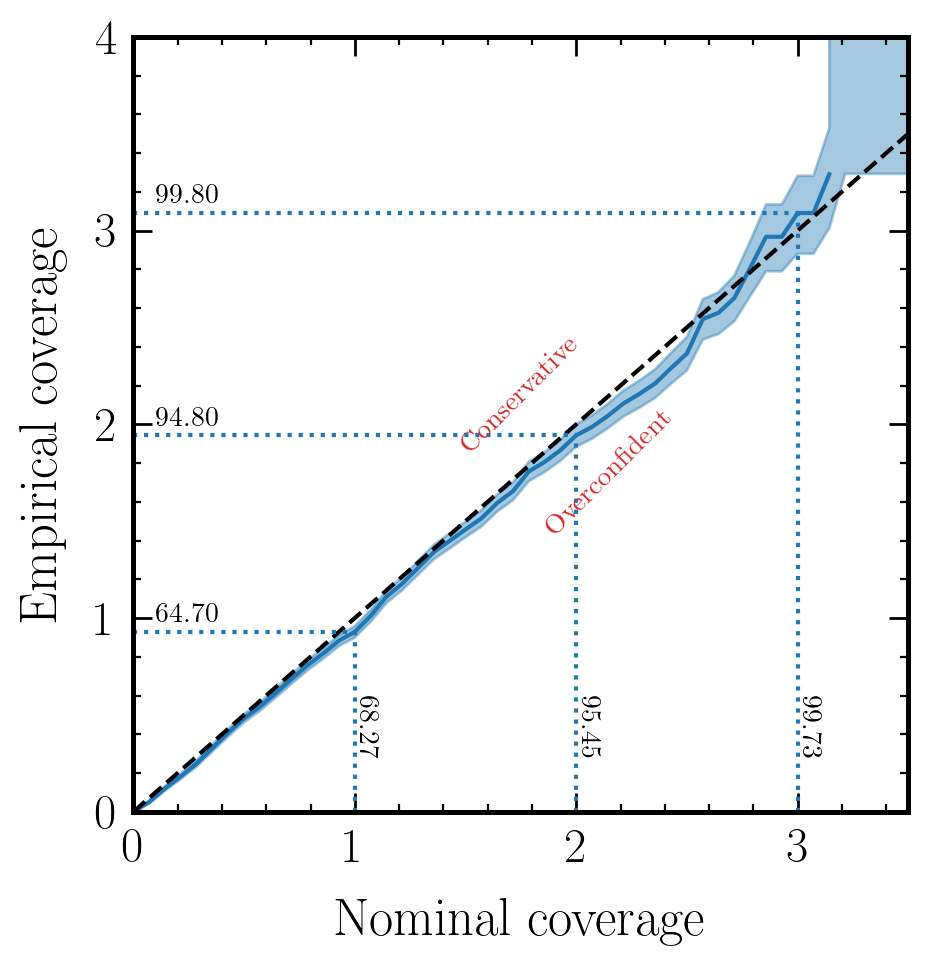
\includegraphics[width=0.5\linewidth]{GL-coverage.png}
    \caption{Empirical versus nominal expected coverage probabilities for the cutoff mass inference network. In case the line lies above (below) the black dashed diagonal line, the credible intervals are conservative (overconfident) and contain the true value with a frequency higher (lower) than nominally expected. We show the empirical (nominal) probabilities as horizontal (vertical) text.
}
\label{fig:coverage}
\end{figure}

We would like to directly test and validate the statistical behaviour of our inference results by determining the expected coverage of the ratio estimator produced by the network. This can be easily done in \swyft thanks to local amortization \citep{Miller:2022shs}.
The goal is to compare the nominal and empirical expected coverage probabilities of estimated Bayesian credible intervals, which should coincide for a well-calibrated estimator. For the statistical formalism and definition of credible region and expected coverage probability, we refer the reader to \cite{Hermans:2021rqv}. In brief, an ideal estimator has matching empirical and nominal expected coverage, a conservative one predicts lower credibility than empirically obtained, and an overconfident one has higher nominal than empirical credibility. In plots like Figure~\ref{fig:coverage}, the line for an ideal ratio estimator should perfectly align with the diagonal, whereas for a conservative (overconfident) estimator, it will lie above (below) the diagonal.
In combination with visually checking the posteriors, this test supports the accuracy of the posterior estimator and is also particularly useful when one does not have access to the ground truth against which to compare the results.
In Figure~\ref{fig:coverage} we show the empirical versus nominal expected coverage probabilities for the cutoff mass inference network. We can see that the inference network for the half-mode mass has converged with good expected coverage. 


\section{Discussion}\label{sec:sl-discussion}

In this section, we discuss the improvements to the model and inference question which need to be addressed before we can safely apply our pipeline to the analysis of real data. 

First, we have neglected effects such as inadequate \emph{lens light} subtraction and assumed the lens light to be known. Regarding the \emph{noise} model, we did not account for correlated pixel noise due to instrumental effects including the telescope's \gls*{psf}, multiband observations, drizzling  (\eg~see \cite{Wagner-Carena:2022mrn}), and even complex noise with an unknown likelihood function.

In this work, we have employed an analytic parameterisation (the Sérsic profile) as a lensed source light distribution model, which is adequate to analyze low-resolution images. However, to accurately model higher-fidelity lensing observations, such as those from on-going (\eg~HST) and future (\eg~JWST, ELT, SKA) telescopes, more \emph{complex source models} need to be employed. Existing models, in order of complexity, are regularised pixellation of the source plane (see, \eg, \cite{Suyu:2006fd, Karchev:2021fro, Vegetti:2008eg}), source modelling through basis functions (\eg~shapelets \citep{Birrer:2018xgm} or wavelets \citep{Galan:2020mnn}) attached to the source plane, and deep learning approaches (see, \eg, \cite{Adam:2022esz, Morningstar:2019szx}).
The ability to accurately and precisely reconstruct the complex morphology of strong-lensing sources is of the utmost importance, as to disentangle the source surface brightness inhomogeneities from the percent-level fluctuations introduced by substructures in the lens. We anticipate that using sources with more complex morphologies will result in higher sensitivity to the DM cutoff mass, provided that it is possible to model these sources. In fact, the residuals between the image of an extended source lensed by the total lens potential (accounting for substructures), and that of the same source lensed only by the main lens component are proportional to the gradient of that source evaluated in the image plane \citep[Equation 16]{Cyr-Racine:2019aa}. 

Regarding \gls*{wdm} modelling, validation of our smoothing scheme (\autoref{subsubsec:smoothing}) is required to accurately account for \gls*{dm} free-streaming effects. Moreover, we should account for uncertainties due to the assumed halo density profile by considering different \gls*{dm} distributions around galaxies (see, \eg, \cite{Salucci:2018aa} for a review). We note that, thanks to its flexibility, our pipeline can incorporate any arbitrary \gls*{dm} model, as long as it specifies the form of the \gls*{hmf} and the density profiles of individual substructures. 
 
Finally, we would like to draw the reader's attention on the fact that in our modeling we assume that the halo mass of the lens is known exactly from its Einstein radius (see \autoref{subsubsec:sl-model-sub}). 
This is a strong assumption that has as a consequence the separation of substructure parameters $\pp$ and lens parameter $\plens$ once we marginalize the posterior probability over the halo mass in Equation~\eqref{eq:model}.
In particular, the second inference question we have addressed in this work in Section~\ref{sec:results-pop}, constraining the cutoff mass of the subhalo mass distribution, is then a simplified version of the real one, which is to simultaneously determine the halo mass and subhalo mass distribution of the lenses from real data (see, \eg, \cite{Birrer:2017rpp}). 

While this work used simple mock lenses, \gls*{tmnre} makes it possible to add realism and parameters to a simulator without significantly altering the inference procedure, or necessarily increasing the simulation budget \citep{Cole:2021gwr}. It should therefore be straightforward to incorporate these various complexities we ignored in this work without fundamentally modifying the inference pipeline. 

%Throughout this study, we have made a number of simplifying assumptions for the, halo mass of the lens, source light profile, and substructure models. We have also neglected effects such as inadequate lens light subtraction, realistic \gls*{psf} modeling, and correlated pixel noise due to effects including the telescope's \gls*{psf}. Before this analysis pipeline can be safely extended to real observations, these assumptions need to be correctly addressed, as discussed in Section~\ref{sec:discussion}. 


\section{Conclusions}\label{sec:sl-conclusions}

Measuring both the individual and collective properties of \gls*{dm} halos on sub-galactic scales by means of their gravitational effect is an important probe of the fundamental nature of \gls*{dm}. One of such probes, strong gravitational lensing, has sparked much interest over the last few years. Moreover, the development of fast and accurate techniques to extract information from strong lensing images is well motivated by the wealth of new high-resolution strong lensing observations that will become available in the near future.

In this work, we have presented the first step towards a new neural simulation based inference pipeline (Chapter~\ref{cha:sbi}) to analyse present and future strong gravitational lensing systems in order to measure the properties of individual \gls*{dm} halos (Section~\ref{sec:results-sub}) and constrain the cutoff in the \gls*{dm} \gls*{hmf}, and so the \gls*{dm} mass (Section~\ref{sec:results-pop}). To this end, we have used a recent machine learning development, \gls*{tmnre}, that makes it possible to \textit{target} the analysis to a specific observation rather than amortize over all possible variations in lensing systems, making inference more efficient and precise. Thanks to \gls*{tmnre}, we overcome the computational challenges of traditional \gls*{mcmc}, nested sampling and trans-dimensional \gls*{mcmc} methods, by directly learning the marginal posterior for the parameter of scientific-interest from the observation. Moreover, \gls*{tmnre} leverages neural networks to directly learn the best summary statistic possible from the full input data, without having to compress the observation into hand-crafted summary statistics, like for \gls*{abc} frameworks. The method is applicable to simulators with unknown likelihood functions and large or even variable numbers of input parameters. Lastly, the resulting inference networks can be poked and prodded to confirm they are statistically well-behaved.
This work is then a step forward towards making the analysis of strong lensing images for \gls*{dm} science faster, more efficient, and more accurate. 

\mbox{}

Our key results can be summarized as follows:

\noindent\textbf{\gls*{tmnre} can recover existing results.} We verified the accuracy of \gls*{tmnre} by confirming it reproduces analytically-calculable posteriors in a toy lensing scenario with known macromodel parameters and subhalo mass (Figure~\ref{fig:gl-sp-post}).

\noindent\textbf{\gls*{tmnre} enables direct marginal inference.} Thanks to marginalized inference, the \gls*{tmnre} based analysis is able to correctly propagate the lens and source parameters uncertainties, and  account for the presence of a population of substructures, when estimating the marginal posterior of interest. 

\noindent\textbf{\gls*{tmnre} enables statistical checks.} Since the inference networks learned by \gls*{tmnre} are locally amortized over a range of potential observations, we were able to test their statistical consistency. Our checks confirm that \gls*{tmnre} on average produces posteriors with the correct width for the macromodel and subhalo parameters. Such tests would be extremely expensive with likelihood-based inference since they would require rerunning the sampling machinery on numerous mock observations.

\noindent\textbf{The perturber population matters.} We demonstrated that the sensitivity with which a subhalo's parameters are measurable can be significantly degraded when marginalizing over a population of perturbers. While the $1\sigma$ regions of our position and mass posteriors were centered on the subhalo's true parameters, they had heavy tails extending to the boundaries of our tight, manually-fixed priors. Given our validation, statistical checks and the fact \gls*{tmnre} is so far the only method capable of performing the high-dimensional marginalization required for this analysis, \emph{our results therefore suggest that the population of light perturbers should not be neglected}. However, it is important to highlight that we cannot strictly conclude from our results that the presence of a substructure population makes the inference of the properties of an individual subhalo unfeasible. What we find is that it makes the task more challenging for our particular \gls*{sbi} approach and network architectures. Whether better network architectures for the ratio estimator capable of modeling the posterior more accurately than \gls*{mlp} Mixer, or maybe the proper handling of the problem with a full trans-dimensional likelihood-based \gls*{mcmc} method dealing with the perturber population can resolve the issue remains open, and an important question to study in future work.
  
\noindent\textbf{\gls*{tmnre} enables hierarchical inference.} We demonstrated that our framework is able to statistically extract the \gls*{dm} cutoff mass signal from a population of small-scale dark matter halos, by performing hierarchical inference on up to 200 observations (Section~\ref{subsec:dm} and Figure~\ref{fig:mhm_results}). What we find is an expected 95\% credible lower limits around 6.5 $\si{\keV}$ in the case of the scenario closest to \gls*{cdm} (see the bottom left panel in Figure~\ref{fig:wdm_results}), given the adopted prior and the various assumptions discussed in Section~\ref{sec:sl-discussion}. 

%Measuring the properties of both individual \gls*{dm} halos and of a population of dark substructures on subgalactic scales is an important probe of the fundamental nature of \gls*{dm}. However, extracting their parameters from observations is difficult for a myriad of reasons, including the fact that lenses contain multiple perturbers (sub-/\gls*{los} halos). In this work we demonstrated that \gls*{tmnre} enables analyses of individual perturbers' properties in scenarios where the application of likelihood-based methods is difficult or infeasible. The key strength of \gls*{tmnre} is its ability to directly learn marginal posterior functions for a set of scientifically-interesting parameters from simulated data. By truncating the range of parameters used to generate the simulations, \gls*{tmnre} enables precision inference of individual observations using a targeted set of training data. This enables the previously-intractable marginalization over large perturber populations. Furthermore, the method is applicable to simulators with unknown likelihood functions and large or even variable numbers of input parameters. The resulting inference networks can be poked and prodded to confirm they are statistically well-behaved.

\mbox{}

A part from the possible framework improvements discussed in Section~\ref{sec:sl-discussion}, an interesting direction for further work is the use of \gls*{tmnre} for model comparison. While here our ratio estimators were trained to compute the likelihood-to-evidence ratio, as pointed out in \cite{Hermans:2019ioj} it is possible to learn other ratios of densities. In particular ratio estimators can be used to learn the Bayes factor for assessing the strength of the evidence for different models. This could be used to determine whether an image contains a perturber or not, and to map the minimum-detectable perturber mass as a function of its position.

Overall, we believe using \gls*{tmnre} to measure individual perturbers and perturbers' population parameters as described in this work provides a promising path towards uncovering the identity of dark matter.

%\section*{Acknowledgements}
%
%We thank Benjamin Kurt Miller and Elias Dubbeldam for helpful discussions.
%
%A.C. received funding from the Netherlands eScience Center (grant number ETEC.2019.018) and the Schmidt Futures Foundation. This work is part of a project that has received funding from the European Research Council (ERC) under the European Union’s Horizon 2020 research and innovation program (Grant agreement No. 864035).
%
%This work was carried out on the Lisa Compute Cluster at SURFsara, which runs on 100\% wind energy.
%
%Software used: \texttt{astropy} \citep{Astropy:2013muo,Astropy:2018wqo}, \texttt{jupyter} \citep{jupyter}, \texttt{matplotlib} \citep{Hunter:2007ouj}, \texttt{numpy} \citep{Harris:2020xlr}, \texttt{PyTorch} \citep{pytorch}, \texttt{pytorch-lightning}\footnote{
%    \url{https://www.pytorchlightning.ai/}
%}, \texttt{seaborn} \citep{Waskom:2021psk}, \texttt{swyft} \citep{Miller:2022shs} and \texttt{tqdm} \citep{tqdm}.
%
%\section*{Data Availability}
%
%The data underlying this article will be shared on request to the corresponding author.


%%%%%%%%%%%%%%%%%%%%%%%%

\begin{subappendices}
% https://tex.stackexchange.com/questions/120716/appendix-after-each-chapter
% https://tex.stackexchange.com/questions/581707/appendix-sections-in-book-class-with-hyperlinks-in-toc

\section{Compression network architectures}
\label{app:architectures}

The compressor architectures are given in Table~\ref{tab:sl-cnn} and Table~\ref{tab:sl-mixer}. Note that we standardize the images before providing them to the networks.

\begin{table}
    \centering
    \begin{tabular}{c}
        \toprule
        \texttt{Conv2d(1, 4, 8, 2, 1, bias=False)} \\
        \texttt{BatchNorm2d(4)} \\
        \texttt{LeakyReLU(0.2)} \\
        \midrule
        \texttt{Conv2d(4, 8, 8, 2, 1, bias=False)} \\
        \texttt{BatchNorm2d(8)} \\
        \texttt{LeakyReLU(0.2)} \\
        \midrule
        \texttt{Conv2d(8, 16, 8, 2, 1, bias=False)} \\
        \texttt{BatchNorm2d(16)} \\
        \texttt{LeakyReLU(0.2)} \\
        \midrule
        \texttt{Conv2d(16, 32, 8, 2, 1, bias=False)} \\
        \texttt{BatchNorm2d(32)} \\
        \texttt{LeakyReLU(0.2)} \\
        \bottomrule
    \end{tabular}
    \label{tab:sl-cnn}
    \caption{The convolutional compression network used in the macromodel parameter ratio estimator. The notation is taken from \texttt{PyTorch}: the arguments to \texttt{Conv2d} are the number of input channels, output channels, kernel size, stride and padding, respectively. The horizontal lines demarcate where the number of channels changes. The output of the network is flattened into a vector with \num{128} features.}
\end{table}

\begin{table}
    \centering
    \begin{tabular}{r l}
        \toprule
        \texttt{image\_size} & \texttt{100} \\
        \texttt{channels} & \texttt{1} \\
        \texttt{patch\_size} & \texttt{10}\\
        \texttt{dim} & \texttt{256} \\
        \texttt{depth} & \texttt{4} \\
        \texttt{num\_classes} & 32 \\
        \texttt{dropout} & \texttt{0.1} \\
        \bottomrule
    \end{tabular}
    \label{tab:sl-mixer}
    \caption{The details of the MLP Mixer compression network in the subhalo ratio estimator. We use the implementation from \url{https://github.com/lucidrains/mlp-mixer-pytorch}, with arguments given in the table.}
\end{table}

\end{subappendices}
